\documentclass[11pt,a4paper]{article}
\usepackage[margin=2.4cm]{geometry}
\usepackage[T1]{fontenc}
\usepackage[utf8]{inputenc}
\usepackage{lmodern}
\usepackage{amsmath}
\usepackage{amssymb}
\usepackage{graphicx}
\usepackage{booktabs}
\usepackage{tabularx}
\usepackage{longtable}
\usepackage{array}
\usepackage{natbib}
\usepackage[hidelinks]{hyperref}
\usepackage{xcolor}
\usepackage{pgfplots}
\pgfplotsset{compat=1.18}
\setlength{\parskip}{4pt}
\setlength{\parindent}{0pt}
% A claim id in the repository's ledger (docs/claims.yaml): every number that carries one is checked by
% scripts/claims.py against a committed artifact (two claims have none and say so), and the marker is how a reader
% finds the check.
% tests/test_claims.py requires every tag here to name a registered claim that is not superseded.
\newcommand{\claim}[1]{{\scriptsize\textsf{\textcolor{gray}{[#1]}}}}
\newcommand{\pkg}{\texttt{olmoearth\_inferenceX}}
\newcommand{\code}[1]{\texttt{#1}}
% placeins' \FloatBarrier, defined here because placeins is not in the TeX installation used: if floats are still
% waiting, put them out before going on, so a table stays in its section.
\makeatletter
\providecommand{\FloatBarrier}{\par\begingroup\let\@elt\relax
  \edef\@tempa{\@botlist\@deferlist\@dbldeferlist}\ifx\@tempa\@empty\else\clearpage\fi\endgroup}
\makeatother

\title{\pkg: confidence-based review, comparison and accuracy estimation for Earth-observation classification maps\\[6pt]
\large Technical report, version 1.20.1}
\author{Ziming Qi\\[2pt] \small \url{https://github.com/2imi9/olmoearth_inferenceX}\\[-1pt]
\small \url{https://github.com/2imi9/olmoearth_inferenceX-record}\\[-1pt]
\small \url{https://olmoearth-inferencex.readthedocs.io}}
\date{27 October 2026}

\begin{document}
\maketitle

\begin{abstract}
This report describes \pkg, a Python package for assessing classification maps from Earth-observation models, and
the record behind it. Without labels, the package ranks a map's windows for review by the model's confidence,
explains each flagged window by label-free cues, and compares two maps with regard to their dates. With a labelled
sample, it estimates the error rate and per-class accuracy with design-based intervals, certifies a high-confidence
zone whose error rate is bounded with a stated probability, and, from labels drawn where two maps differ, names the
more accurate map by an exact test and gives an interval on their accuracy difference. Read through linear probes on OlmoEarth Base's frozen embeddings, the confidence margin
closes a median 0.68 of the gap between a random and a perfect review order on the 24 tasks of the model authors'
embedding suite, and a review of the least confident 10\% holds a median 0.214 of the errors, about twice a random
10\%; it beats a random order in all 3,560 cells of sixteen encoders, their tasks and ten probe seeds, and beats
informative no-model controls on three references produced outside this project. On a re-run of Ai2's deployment configuration for its fine-tuned AWF model, the
confidence ranked the map's errors with an AUROC of 0.849 at Ai2's expert-placed validation points but, under a
one-to-one crosswalk, 0.638 on 2017 imagery at the plots of an independent random sample around the area that had
input, below the preregistered 0.70; the record's own fine-tune of the task on OlmoEarth v1.2 repeated both verdicts
(0.814 and 0.642). That run changed the year, the place, the legend and the kind of point at once and cannot say which
weakened the ranking; a report-only reading found most of its confident errors on one grass/shrub boundary that neither
legend defines. A preregistered blind test at 890 fresh plots of the same sample, more than 100\,km from the area, did
not repeat the miss: the v1.2 fine-tune's confidence ranked its errors at 0.729 (90\% interval 0.701 to 0.758, its
lower end on the bar), and Ai2's v1 checkpoint, which did not reproduce its earlier predictions under the current
rslearn, was reported only. On a second task, Ai2's Forest Loss Driver model at a stratified sample of 689 Amazon alerts
MapBiomas Alerta published in 2026, the confidence ranked the disagreements at 0.770, at or above the bar of 0.70 on the point value
(interval 0.682 to 0.855); post hoc, the 53 disagreements in which the model chose a class the reference does not
record ranked at 0.945 and the 18 confusions between the two classes the alerts were sampled from at 0.400, below
chance and as confident as the correct alerts. On another
organisation's deployed product outside land cover, FTW's global field map at 1,295 benchmark test chips in four
European countries, the map's own probability ranked its window errors at AUROC 0.837 to 0.936, meeting the
preregistered bar in 3 of 4 countries, and the labelled routes kept their guarantees. On three published
products, disagreement with a second product flagged their confident errors four to five times as often as their
confident correct rows on two and 1.45 times on the third, short of the preregistered twofold on all three. On PASTIS, a probe read without the
optical input it was trained with erred confidently (59.8\% of its errors as confident as the median correct window,
against 6.0\%), though not on CropHarvest China 6; given a raster of input conditions, the package therefore ranks,
samples and certifies each condition on its own. The random-sample interval is exact; it remains valid when a reviewer cannot judge some windows, and
widens to sharp bounds for a reviewer whose error rates the user states; the bounds, their sharpness and the transfer
of coverage are proved in Lean (proofs archived at v1.9.0 and not built by the continuous integration), and the
monotonicity of the package's own intervals is checked numerically. The certified zone met its
guarantee on all 110 graded cells. Over 2,514 pairs of encoder maps, 100 labels drawn among the windows where two maps
differ named the more accurate map on 60.3\% of draws, against 12.7\% for 100 labels drawn from the whole map; on the
1,709 pairs that differ on more than 100 windows, where the labels are a sample rather than all of them, 42.8\%
against 11.3\%. Against McNemar's test on a whole-map sample of the same 100 labels, on nine pairs of published products,
the design named the better-agreeing map at least as often on 8 of 9 pairs against the exact form but on only 6 against
Foody's z form, short of its preregistered 7; the three losses were on pairs differing by under 1.2 points. On two published land-cover products graded against an independent probability sample of 25,000
plots, the error-rate interval held its coverage, labels drawn where the products differ never named the one less in
agreement with the reference (they named one on 6\% to 29\% of draws at 50 to 200 labels), and LCMAP's own
confidence ranked its errors with an AUROC of 0.75; certified zones on that confidence met their guarantee in every
cell, and at 300 labels the default rule returned no zone on 87\% of draws at $\alpha$ half the error rate, though 65\%
of the plots lie in a zone within it.
Given an agency's stratified reference sample, the package reproduces the published overall accuracies of NLCD 2016's
assessment (86.39\% against 86.4\%) and GFC2020's, each with a stratified betting interval valid in finite samples,
with no large-sample approximation, and 1.60 to 1.64 times as wide as the agency's normal-theory interval; at NLCD's
design shape the normal-theory intervals covered below 0.9408 (0.95 less three Monte Carlo standard errors) on 33 of
91 quantities, all of them per class, and the valid ones on none.
The record comprises 121 experiment scripts covering 99 experiment numbers from exp01 to exp118 (exp117's design study
is in a folder of its own), and 291 ledger claims, 289 of them checked against a committed artifact and 154 by an
independent second route, and reports failed predictions as failed.
\end{abstract}

\section{Introduction}

A classification map from an Earth-observation model is usually applied where no reference labels exist. This
report addresses five questions: which windows to review first when only a fraction can be checked; how two maps of
one area differ, when they come from different crops, backbones, sensors, encoders, training states or dates; once
some windows are labelled, how wrong the map is, how accurate each class is, and which part of it can be used with a
stated error bound; which of two maps is more accurate, from as few labels as possible; and what an agency's published
stratified reference sample says about a map, with intervals that hold at its sample size.

\pkg{} ranks $4\times4$-pixel windows by the model's confidence margin with label-free cues (Section~\ref{sec:ranking}),
compares two maps with regard to their dates (Section~\ref{sec:compare}), estimates error rates and per-class
accuracies from a labelled sample (Section~\ref{sec:estimate}), certifies a zone of the most confident windows
(Section~\ref{sec:zone}), estimates the accuracy difference of two maps from labels where they differ
(Section~\ref{sec:whichmap}), and grades a map with an agency's stratified reference sample
(Section~\ref{sec:agency}). It reads arrays and rasters and loads no model, and it serves the same commands to a
language-model agent (Section~\ref{sec:interfaces}); Figure~\ref{fig:overview} shows the six outputs that work on a map's windows; \code{grade}, which reads an agency's
points, is not drawn. In the
evaluation the label-free readings are graded against labels and never fitted to them \claim{labels-grade-never-train}.

\begin{figure}[t]
\centering
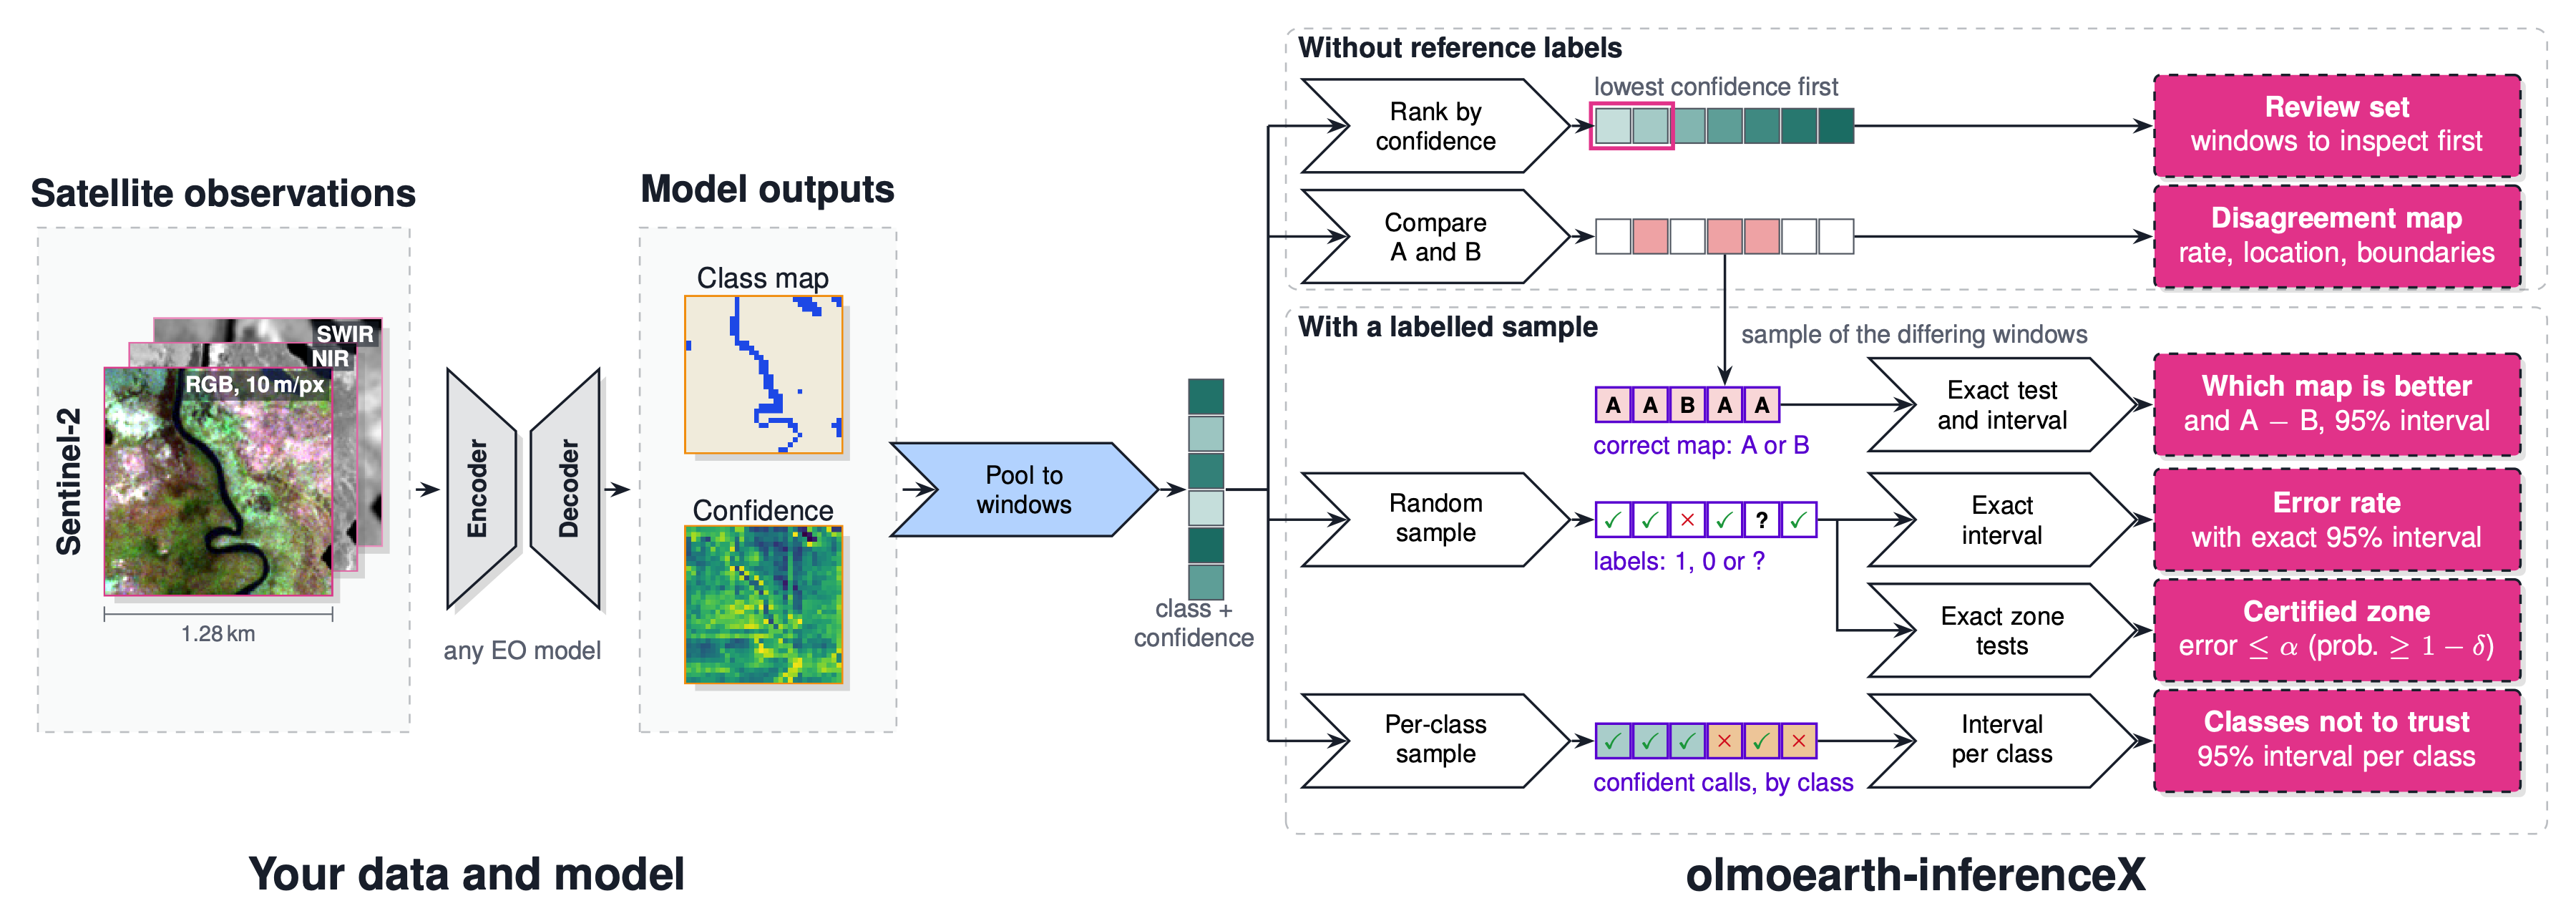
\includegraphics[width=\linewidth]{../docs/figures/architecture.png}
\caption{The structure of the package. It reads a model's class scores (and optionally a second map and a raster of
input conditions), pools them to windows that each carry a class and the model's confidence, and answers two kinds of
question. Without labels, it ranks the windows by confidence into a review set (Section~\ref{sec:ranking}) and
compares two maps (Section~\ref{sec:compare}). With a labelled sample, windows drawn at random give the error rate
with an exact interval (Section~\ref{sec:estimate}) and, by exact tests on the most confident zones, a certified zone
(Section~\ref{sec:zone}); windows drawn where two maps differ name the more accurate map by an exact test and give
the accuracy difference (Section~\ref{sec:whichmap}); and a sample of each class's confident calls gives each class's
error and the classes not to trust (Section~\ref{sec:audit}). Each step runs per input condition when a condition
raster is given.}
\label{fig:overview}
\end{figure}

\paragraph{Relation to prior work.} No component is new in isolation. Risk-coverage evaluation comes from selective
classification \citep{chow1970,geifman2017,geifman2019}, softmax confidence as the error-detection baseline from
\citet{hendrycks2017} and \citet{jaeger2023}, and the margin from margin sampling \citep{scheffer2001,lewis1994}; related
measures are \citet{rottmann2020} and \citet{meyer2021}. The estimators follow design-based map-accuracy practice
\citep{olofsson2014,stehman2019}, with the cluster-sampling correction of \citet{stehman1997}; stratifying a classifier's
evaluation sample by its confidence was proposed by \citet{kumar2016}, and prediction-powered inference
\citep{angelopoulos2023ppi}, including a design-based spatial form \citep{shirota2026} and applications to
remote-sensing maps \citep{lu2024regression}, addresses the same estimation
task. The intervals for an agency's stratified sample are built from the exponential-supermartingale and betting
intervals for sampling without replacement \citep{waudbysmith2020,waudbysmith2024,stark2023alpha}, related to the stratified tests of risk-limiting audits
\citep{ottoboni2018,spertus2022}, and are reported beside the design-based estimates of \citet{stehman2014}
(Section~\ref{sec:agency}). The certified zone follows risk control by exact tests \citep{bates2021,angelopoulos2021}. Disagreement maps
between land-cover products \citep{fritz2008} and paired accuracy tests on a shared sample \citep{foody2004} precede the
comparison of two maps, and the bounds for a reviewer who errs are the partially identified form of the correction of
\citet{rogan1978}. \citet{lehmann2026} report that geospatial foundation models grow overconfident under corruption
and that confidence-based abstention cannot defer around their confidently wrong predictions; this record has applied
no corruption, and besides exp88's missing input (Section~\ref{sec:res-conditions}) two tests under a shift of year
and place: a deployed model graded at a random sample near its area (Section~\ref{sec:res-deployed}), and a
preregistered blind test at fresh plots farther away, which did not repeat that test's miss
(Section~\ref{sec:res-blind}). This work joins these parts in one after-the-fact tool
for maps from Earth-observation foundation models and tests the known signals against the model's confidence and
against controls that do not use the model.

\section{Methods}
\label{sec:methods}

\subsection{Windows, the confidence signal and the ranking}
\label{sec:ranking}

Pixels are grouped into windows of $4\times4$ pixels, the unit of ranking, comparison and estimation. A window's
decision is the majority class of its pixels, and a tie goes to the class whose voting pixels are more
confident. For a pixel with logits $z_{(1)} \ge z_{(2)} \ge \dots$, the confidence is the margin
\begin{equation}
  m = z_{(1)} - z_{(2)},
\end{equation}
and for a binary logit map the absolute logit $|z|$. For a probability map it is the top class probability, which ties
where probabilities saturate. The option \code{form="top1"} ranks a multi-class logit map by the window mean of
$\log p_{(1)}$, computed from the logits without ties. Otherwise a window's confidence $m(w)$ is the pixel confidence
averaged over the window, and its suspicion is $\sigma(w) = -m(w)$. Except exp89, which graded the package's top-1
form on single points, the experiments of Section~\ref{sec:results} graded the margin between the two highest
window-mean class probabilities; the package's per-pixel forms on windows were graded on the seven segmentation tasks
only \claim{window-aggregator-is-not-the-lever}.

A window is a boundary window when any of its eight neighbours has a different decision. The confidence order sorts
windows by decreasing suspicion; the boundary-first order takes the boundary windows first, each group by suspicion.
The review set at budget $b$ is the first $\max(1, \mathrm{round}(bN))$ of the $N$ valid windows. Each flagged window
carries the cues it satisfies: boundary, low confidence (the least confident fifth), tiling instability (a changed
decision under a two-pixel crop shift) and, for water maps, spectral ambiguity. A cue's enrichment, its share among
error windows over its share among correct windows, is quoted as measured on labelled data; since version 1.3.0 the
boundary cue is quoted with the range measured on the suite and the map's own boundary prevalence.

\textbf{Input conditions.} A map can be read from different inputs in different places, for instance radar alone
under cloud and radar with optical imagery elsewhere. Given an integer raster of input conditions on the map's grid
(\code{-{}-condition}, since version 1.4.0), \code{assess} writes a review set per condition, and \code{sample},
\code{estimate} and \code{certify} treat each condition as its own population. Without it, the output notes that
confidence ranked across input conditions can place a model's confident errors late (Section~\ref{sec:res-conditions}).

\begin{figure}[t]
\centering
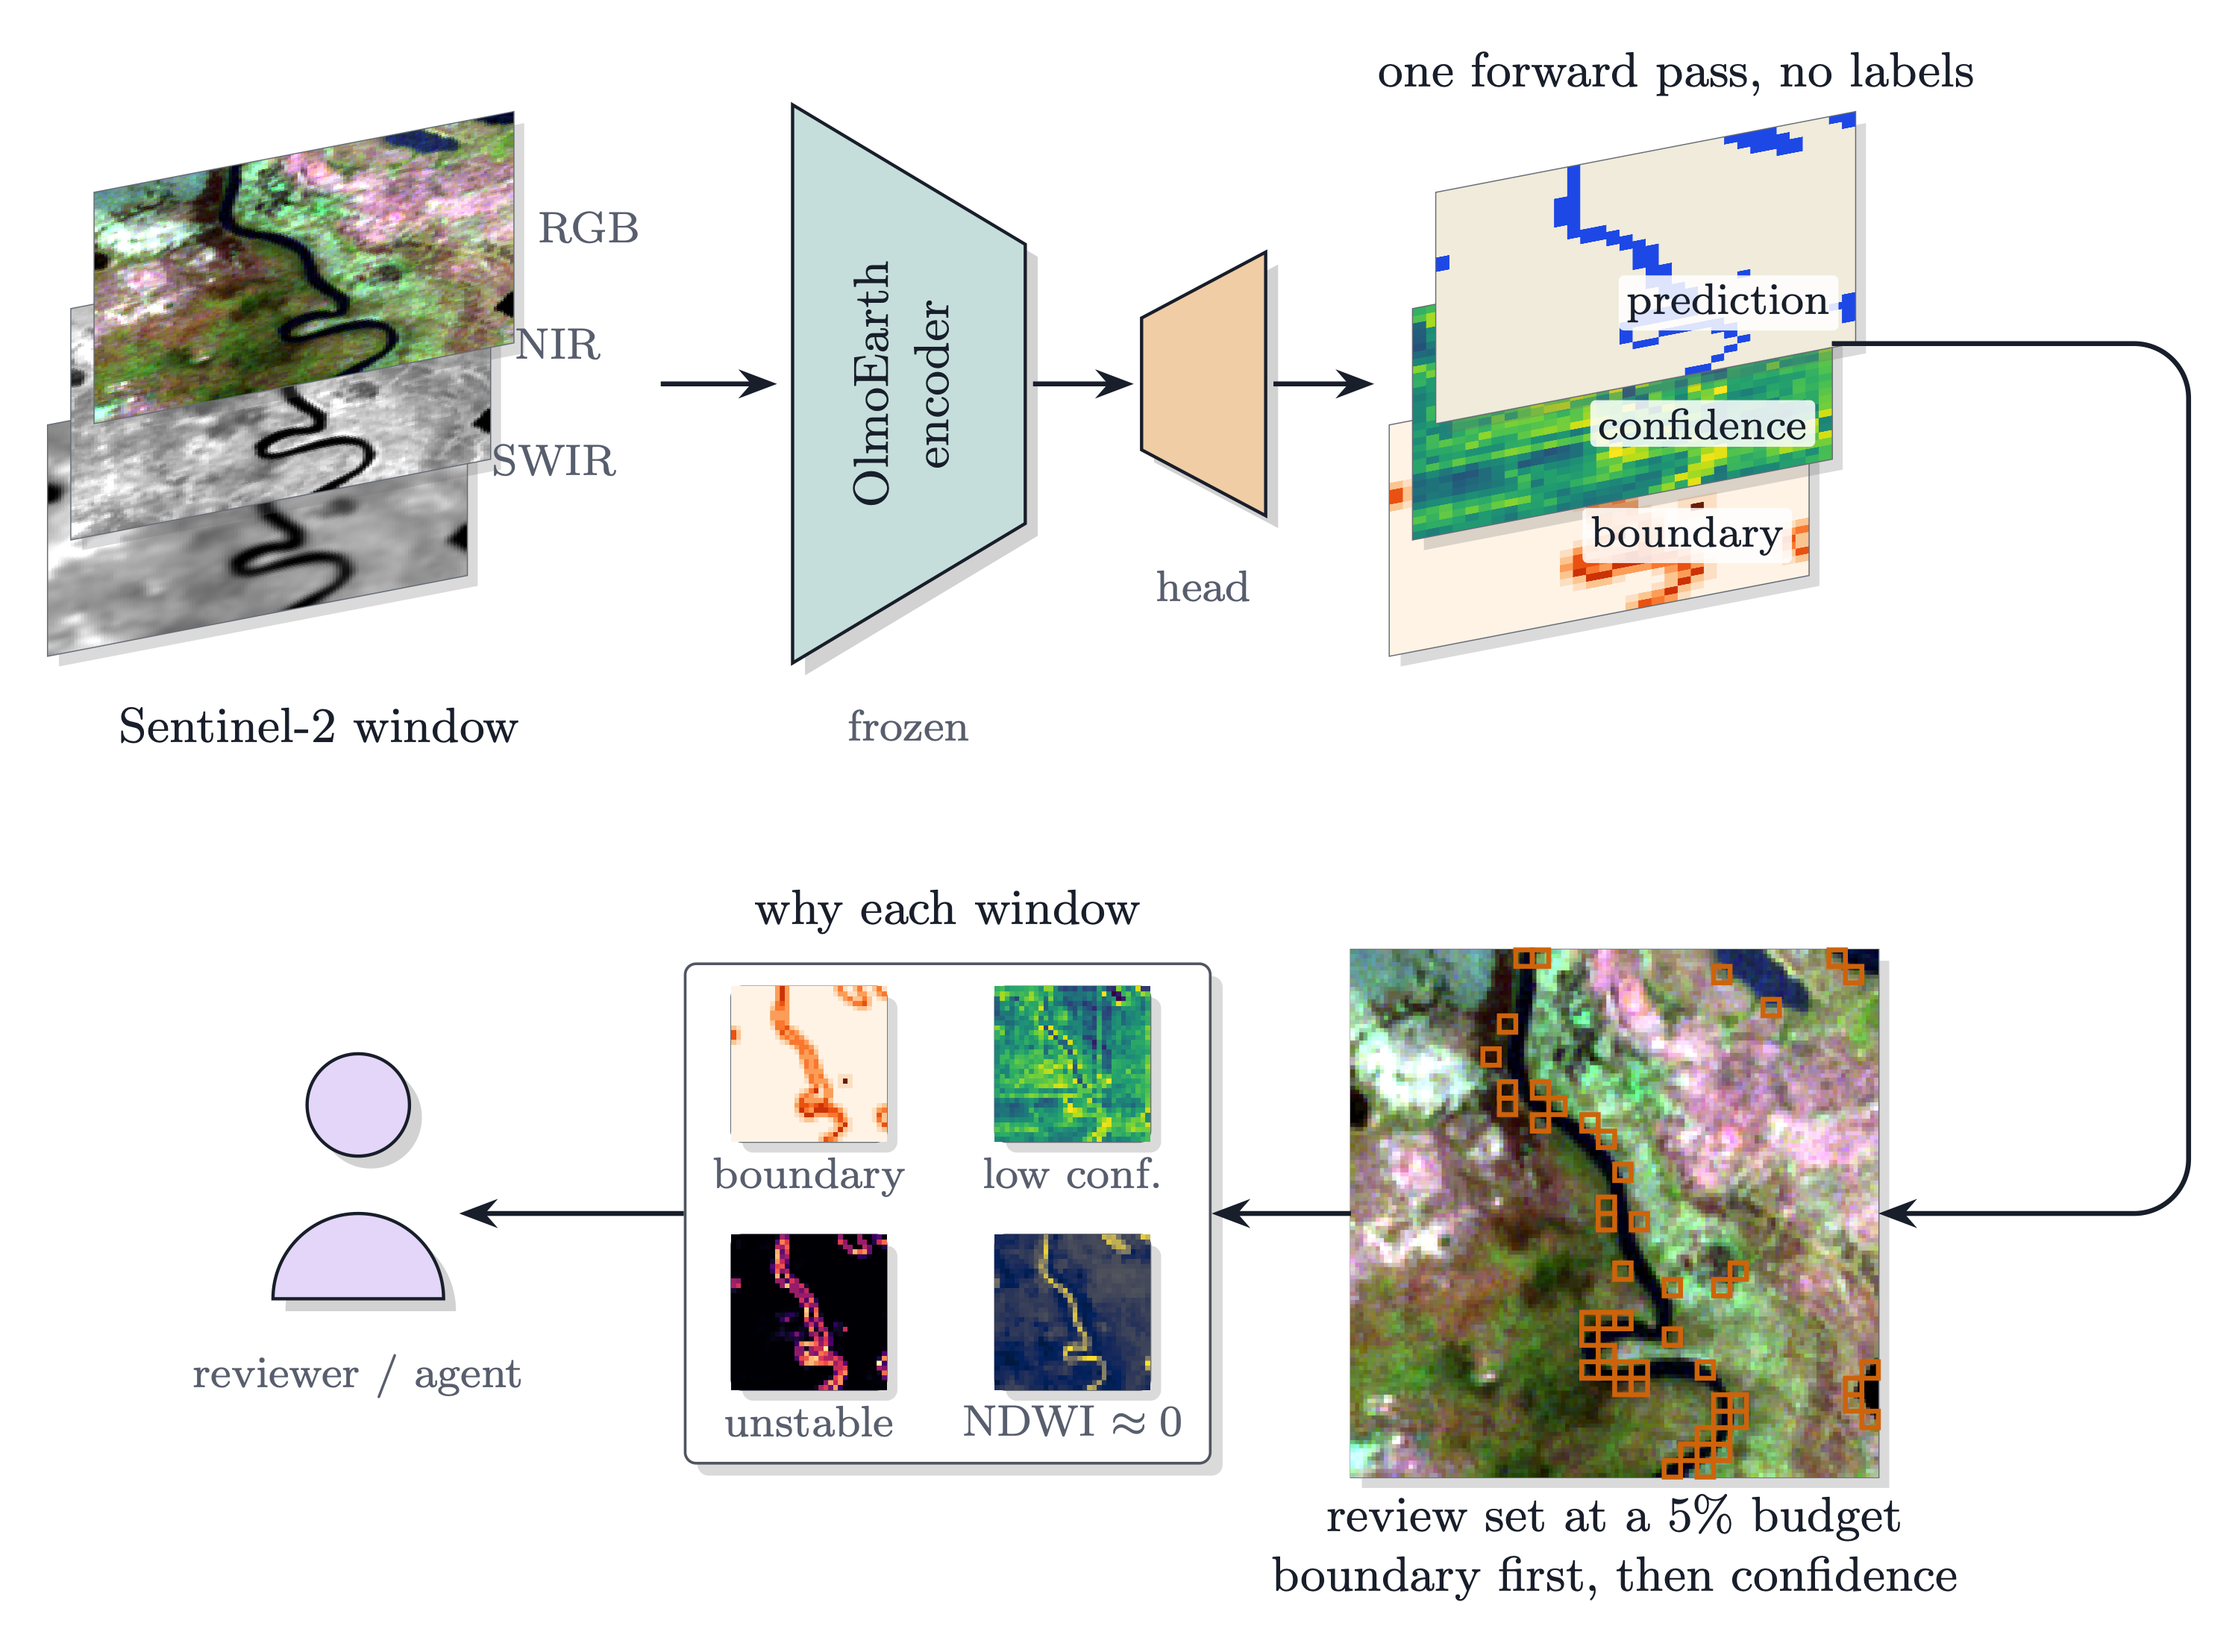
\includegraphics[width=0.92\linewidth]{../docs/figures/pipeline.png}
\caption{One scene through the label-free assessment: Sentinel-2 bands, the frozen OlmoEarth encoder and a task head,
the prediction with its confidence and boundary layers, the review set at a 5\% budget, and the cues per flagged window.}
\label{fig:pipeline}
\end{figure}

\subsection{Comparison of two maps}
\label{sec:compare}

For hard window decisions $A$ and $B$ of two maps on one grid, over the windows $V$ both predict, the package reports
without labels the disagreement rate $|\{w \in V : A(w) \neq B(w)\}| / |V|$, pooled and per group (tile, event or
zone), the enrichment of each cue among differing windows, and the $\phi$ coefficient between two disagreement masks,
which measures whether two differences occupy the same windows. A rate is read against the reseed floor, the rate at
which refitting the head with another seed changes decisions. With a full label raster, a separate block adds the
cross-tabulation of the two error maps and the share of differing windows on which each map matches the label.

Each map may carry the date or period it represents. At one time a difference implies an error in at least one map;
across times it may be change on the ground, and the package then grades which map is right only when the labels' date
is given, reporting which map the labels match in time; with one date stated, grading is refused. Without labels the
package does not decide which map is right; with a sample of labels it says which is more accurate
(Section~\ref{sec:whichmap}).

\begin{figure}[t]
\centering
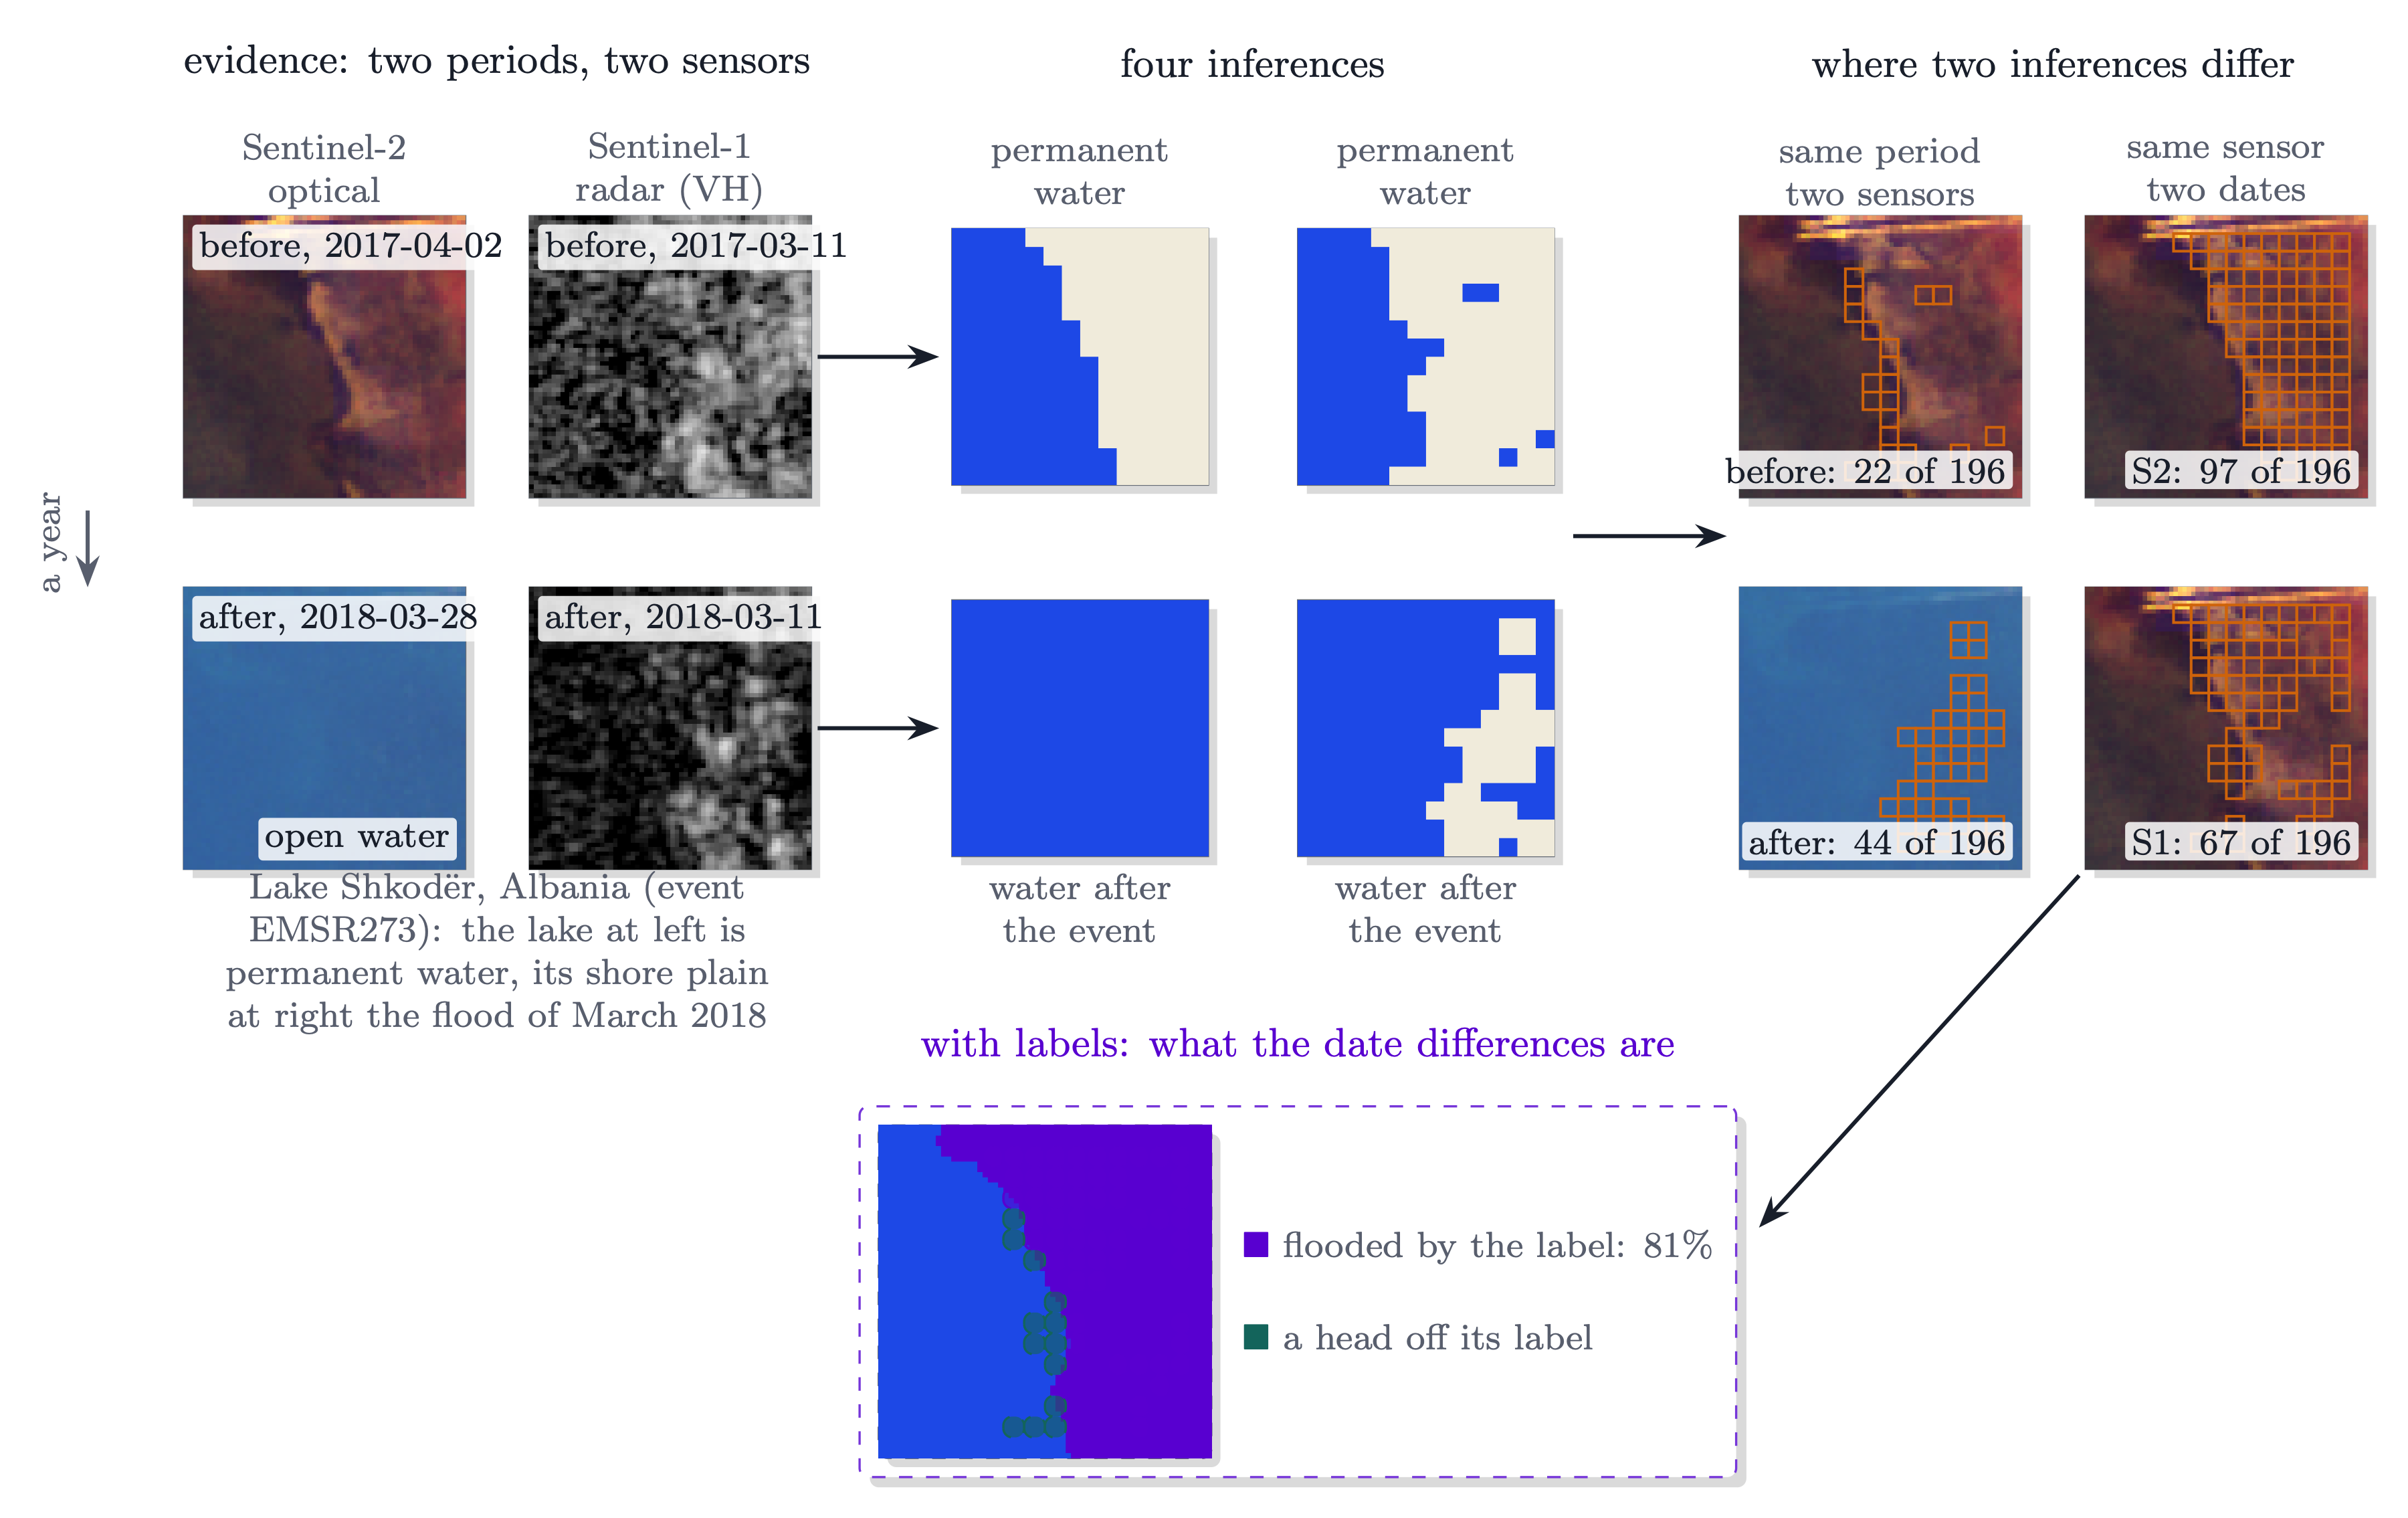
\includegraphics[width=0.92\linewidth]{../docs/figures/compare.png}
\caption{Four dated inputs of one GEOID-Flood chip, each read on identical windows: the same-period and same-sensor
differences on the scene, with the comparison against labels shown separately.}
\label{fig:compare}
\end{figure}

\subsection{Design-based estimation}
\label{sec:estimate}

Let the map have $N$ valid windows, $e_i = 1$ where the map's class differs from the reference class, and
$\theta = N^{-1}\sum_i e_i$. A reviewer labels $B$ windows under one of five designs.

\textbf{Confidence-stratified design (default).} Five strata are cut at the quintiles of the margin, with sizes $N_h$
and weights $W_h = N_h/N$. The budget follows Neyman's allocation, which minimises the variance of the stratified
estimate at a fixed budget,
\begin{equation}
  n_h = B \, \frac{N_h S_h}{\sum_j N_j S_j}, \qquad S_h \approx \sqrt{q_h (1 - q_h)},
\end{equation}
where $q_h$ is the mean of $1 - p_{(1)}$ in stratum $h$, floored at 0.02, and each stratum receives at least two
labels. With $p_h$ the error share among stratum $h$'s labels and $f_h = n_h/N_h$,
\begin{equation}
  \hat\theta = \sum_h W_h \, p_h, \qquad
  \hat v = \sum_h W_h^2 (1 - f_h) \, \frac{p_h (1 - p_h)}{n_h - 1},
\end{equation}
both unbiased under stratified sampling without replacement, with Wilson's interval at the effective sample size
$\hat\theta(1-\hat\theta)/\hat v$, after the effective-sample-size approach of \citet{korn1998}. This interval is
nominal: it has no finite-sample guarantee, and its coverage is known from simulation only. The proportional design
uses the same strata, allocates the budget by stratum size, and has the same estimator and interval.

\textbf{Simple random design.} The sampled error count $k$ is hypergeometric, and the interval for $\theta = K/N$ holds
every $K$ whose two tail probabilities at $k$ both exceed 0.025, widened if needed to contain $k/n$; its coverage is at
least 95\% for every $(N, K, n)$. The package has printed this exact interval since version 1.3.0, in place of the
finite-population Wilson interval that the experiments of Section~\ref{sec:res-estimate} graded.

\textbf{Condition design.} With $L$ input conditions, the budget is split equally across them, a condition too small
for its share being labelled in full, and the model's confidence is not read. Each condition $c$ gets the exact
interval $[\ell_c, h_c]$ at 95\%. The whole-map interval is $[\sum_c W_c \ell'_c, \sum_c W_c h'_c]$, where
$[\ell'_c, h'_c]$ is condition $c$'s exact interval at $1 - 0.05/L'$, $L'$ counts the conditions not labelled in full,
and the sums are taken in exact fractions. By the union bound it covers at least 95\% for every population and
allocation. A stratified Wilson interval with the conditions as strata is not used, because it can cover far less when
a large clean condition sits beside a small degraded one.

\textbf{Tile design.} Tiles are taken in a random order and up to 16 windows labelled in each until the budget is met,
from at least five tiles. With $n_i$ the valid windows of sampled tile $i$, $\bar y_i$ the error share among its
labels and $\bar n$ the mean of the $n_i$, the estimate is the ratio $\hat\theta = \sum_i n_i \bar y_i / \sum_i n_i$
with ultimate-cluster variance $\sum_i n_i^2 (\bar y_i - \hat\theta)^2 / (t(t-1)\bar n^2)$ over $t$ tiles and a $t$
quantile, reported beside the independent-sample interval; its variance ratio to simple random sampling is the design
effect. This interval has no guarantee.

\textbf{Windows the reviewer cannot judge.} A reviewer may enter \code{?} for a window that cannot be judged and keep
its row. With $u$ such windows among the labels, the interval runs from the lower end computed with every \code{?}
counted right to the upper end computed with every \code{?} counted wrong; under a random sample this is
$[L(k), U(k+u)]$. Because both ends of the exact interval move one way with the error count, the result contains the
interval the true labels would give, so it covers at least 95\% however the unjudged windows were chosen, including
by an adversary who sees the truth. Under the confidence and proportional designs any \code{?} switches the interval to
the union bound over strata, and most of the extra width then comes from that switch. The tile design and per-class
accuracy refuse \code{?}.

\textbf{A reviewer who errs.} Let $e_0$ be the share of truly correct windows that the reviewer marks wrong and $e_1$
the share of truly wrong windows that the reviewer passes. The error rate $p$ of the reviewer's labels then satisfies
$p = \theta(1 - e_1) + (1 - \theta) e_0$. If the user states bounds $e_0 \le E_0 < 1$ and $e_1 \le E_1 < 1$, then
\begin{equation}
  \max\Bigl(0, \frac{p - E_0}{1 - E_0}\Bigr) \;\le\; \theta \;\le\; \min\Bigl(1, \frac{p}{1 - E_1}\Bigr),
\end{equation}
and both ends are attained, so the bounds are sharp. \code{estimate -{}-reviewer-false-alarm} $E_0$
\code{-{}-reviewer-miss} $E_1$ maps the interval's ends $[L, U]$ through these increasing functions, so the widened
interval covers $\theta$ whenever $[L, U]$ covers $p$; the rates are the user's statement and are not measured. The
bounds, their sharpness, the transfer of coverage and the step from monotone interval ends to the \code{?} interval are
proved in Lean~4 \citep{demoura2021} with Mathlib \citep{mathlib2020}; the proofs were archived from the main branch
on 10 October 2026 and are in the \code{lean/} folder at tag \code{v1.9.0}
(\url{https://github.com/2imi9/olmoearth_inferenceX/tree/v1.9.0/lean}). The proofs do not cover the monotonicity of
the package's own intervals, which the tests check numerically, and the continuous integration does not build them.

\textbf{Review-set check.} Labelling the review set gives the error share $\mathrm{capture}(b)\,\theta/b$, where
$\mathrm{capture}(b)$ is the set's share of all errors. Windows labelled without a design are accepted as a random
sample only if their mean suspicion percentile is no more than four standard deviations above 0.5, a test for a review
set's enrichment, and since version 1.16.0 no more than four below it, which refuses labels drawn from the confident end
of the map. Passing the check does not make labels a random sample: labels clustered by tile pass it.

\textbf{Per-class accuracy.} With map class $m$ and reference class $r$, the user's accuracy is
$\mathrm{UA}_c = \#\{m{=}c, r{=}c\}/\#\{m{=}c\}$, the producer's accuracy $\mathrm{PA}_c = \#\{m{=}c, r{=}c\}/\#\{r{=}c\}$
and the error-adjusted share $A_c = \#\{r{=}c\}/N$. Under a random sample $\mathrm{UA}_c$ has the exact interval, and
since version 1.14.0 so do $A_c$, by a hypergeometric interval at $1 - 0.05/L$ for $L$ classes, and $\mathrm{PA}_c$
\citep{olofsson2014}, from exact intervals for its two counts at $1 - 0.05/(2L)$ bounded by the map's own count, so
that the shares hold together, and the producer's accuracies, with probability at least 0.95 (exp115); under the
confidence design each is a ratio of Horvitz--Thompson (inverse-probability-weighted) totals with a linearised
variance. Warnings
mark classes with fewer than 30 labels, thin or near-census sampling, one to four sampled errors, or no prediction.

\textbf{The class design.} Since version 1.17.0, \code{sample -{}-design class} stratifies by the map's own class, as
\citet{olofsson2014} advise for accuracy and area: every class gets a floor of labels (50 by default, or all its
windows) and the rest of the budget goes in proportion to class size. Each class's labels are a simple random sample
of it, so its user's accuracy has the exact interval and the whole-map error rate the union bound over the classes.
The count of each reference class in each stratum has an exact hypergeometric interval at $1 - 0.05/(LS)$, with $S$ the
strata not labelled in full; the class areas and producer's accuracies are monotone in those counts and bounded by
them, so all of them hold together with probability at least 0.95, and the points beside them are Olofsson's
stratified estimates. \code{certify} certifies a zone in each class, with $\delta$ split over the classes tested. The
tests compute the coverage exactly over the stratified draw on 45 small maps, with a negative control that shows the
computation can see an interval that is too narrow; exp116 grades the design on real maps
(Section~\ref{sec:est-results}).

\textbf{An interval valid at every sample size (\code{-{}-valid}, 1.20.0).} The intervals above are exact under a
random sample and approximate or union bounds under the others. Since 1.20.0, \code{estimate -{}-valid} prints beside
each design's own interval one that holds at every sample size: a census where every stratum is labelled in full, the
exact hypergeometric interval where one stratum is labelled in part, and otherwise the stratified betting interval of
Theorem~1 (Section~\ref{sec:agency}) with the strata labelled in full added exactly, a \code{?} window read as right
at the lower end and wrong at the upper. With \code{-{}-per-class} each class's user's accuracy, producer's accuracy and
share get such an interval by post-stratification on the map's class, each on its own. It is opt-in and refused on the
tile and audit designs; its tests enumerate every population and draw of small stratified maps. Its measured width is
exp119's (Section~\ref{sec:res-agency}).

\subsection{The certified zone}
\label{sec:zone}

Windows are ordered by decreasing margin, ties by index; the zone at coverage $c$ is the first $n_c =
\mathrm{round}(cN)$ windows, and its risk $R(c)$ is the error rate inside it, for $c \in \{0.05, 0.10, \dots, 1.00\}$.
From a simple random sample of $B$ labels, of which $b_c$ fall in the zone and $k_c$ of those are errors, the exact
one-sided p-value against $R(c) > \alpha$ is
\begin{equation}
  p_c = P(X \le k_c), \qquad X \sim \mathrm{Hypergeom}\bigl(n_c,\ \lfloor \alpha n_c \rfloor + 1,\ b_c\bigr).
\end{equation}
A rule returns a coverage $\hat c$ or no zone and is valid when $P(R(\hat c) > \alpha) \le \delta$ over the draw. The
prefix rule accepts coverages from the smallest upward while $p_c \le \delta$; it is fixed-sequence testing, valid on
any map whatever the shape of $R(c)$ \citep{angelopoulos2021}. The Bonferroni rule accepts every coverage with
$p_c \le \delta/J$ over $J$ levels; it can certify more than the prefix rule when the most confident windows hold
errors. Until version 1.4.0 the package, and until 3 October 2026 the ledger, described the prefix rule as valid only
where $R(c)$ does not decrease with $c$; that condition is not needed, and a test enumerating every error pattern of small maps confirms both rules on
patterns whose risk falls as the zone grows. In the large-zone limit a zone with no errors needs about
$\lceil \ln\delta / \ln(1-\alpha) \rceil$ labels (fewer on a small zone), 45 at $\alpha = 0.05$ and 255 at
$\alpha = 0.009$ for the default $\delta = 0.1$; levels whose expected number of labels, $cB$, is below that are dropped
before any label is read. The package refuses designs other than random or condition and labels that look like a
review set, and certifies nothing outside the zone. A p-value within a relative $10^{-9}$ of its level is decided in exact rational arithmetic,
so that the same labels give the same zone on every C library.

Since version 1.16.0 a zone fixed before labelling, \code{sample -{}-target} $c^*$, is certified by a fallback
procedure \citep{wiens2003,wiens2005}: the target level holds $0.8\delta$, the smaller levels tested share the rest (all
of $\delta$ goes to the target when none is tested), a level that passes hands its share up to the next, and larger
levels are reached only through that hand-up. It is valid on any map, as the prefix and Bonferroni rules are (the
tests enumerate every error pattern of small maps and every draw), and with the target right it needs about half the
labels the Bonferroni rule needs for that zone. $\delta$ bounds the probability, over the draw, that the statement
is wrong, counting the draws that certify nothing. Given that a zone was certified, the chance that it is wrong can
exceed $\delta$, most where a zone's error rate lies just above $\alpha$, where certifying is rare; since 1.17.0 every
output that certifies a zone says so. $\alpha$, $\delta$, the rule and the level cut must be chosen before any label,
since a second run on the same labels is a second test; a sample drawn for a certificate fixes them with the draw
(Section~\ref{sec:certificate}).

With input conditions, the $L$ conditions holding at least the minimum at the undivided $\delta$ are fixed before any
label is read (at $\delta/L$ such a condition may still certify nothing), each is certified inside itself at
$\delta/L$, and the union of their zones errs at most $\alpha$ except on at most $\delta$ of
samples. \code{certify} counts every \code{?} as wrong, which can only certify less. It takes no reviewer error rate:
testing at $\alpha(1 - E_1)$ is valid only if the miss rate holds inside every zone the test can certify, where a
model's confident errors sit. In a construction from a review of 2 October 2026, misses placed in the confident half
of a map, with a whole-map miss rate of exactly $E_1$, certified on every draw a zone that was wrong 10\% of the time
at $\alpha = 5\%$.

Since 1.20.0 the same construction gives a verdict per part of a map. \code{sample -{}-design profile} fixes, from the
map alone before any label, at most twelve profiles (cells of a confidence band, an input condition, the map's class
and a grid block, the small cells folded into one), and labels each at random; \code{certify} on that sample gives each
profile labelled in part an exact two-sided hypergeometric interval at $1 - \delta/L$ and calls it good when the
interval lies at or below $\alpha$, bad when above, and undecided otherwise, so all $L$ verdicts are right together
except on at most $\delta$ of samples (a profile labelled in full compares its rate exactly). The package's tests
enumerate every error pattern and draw of small maps; the verdicts have not been run on a real map.

This guarantee is for one sample whose size is fixed before labelling, read once. Rerunning \code{certify} as labels
are added runs a new test at each look, and the chance that some look certifies a wrong zone grows with the looks
(Section~\ref{sec:zone-results}). Since version 1.8.0 a sequential sample keeps the guarantee at every look.
\code{sample -{}-design sequential} draws a fixed random order of the windows, any prefix of which is a simple random
sample, and fixes before any label the anchor, the smallest zone tested: by default the smallest grid level whose zone
expects enough labels at a stated first budget to be certified with no error among them, at most 0.25. Each level is
tested by an e-process, the mixture with equal weights over the counts $M < M_0 = \lfloor \alpha n_c \rfloor + 1$ of
the likelihood ratios of sampling without replacement against $M_0$ \citep{robbins1970}, in closed form one
hypergeometric tail; it is a supermartingale under every count $M \geq M_0$, so by Ville's inequality \citep{ville1939}
it ever reaches $1/\delta$ with probability at most $\delta$, whatever decides when labelling stops. Levels are tested
in a fixed sequence from the anchor outward \citep{bauer1991}, valid at every look because every test in it is
\citep{tamhane2010}; a passed level stays passed, so more labels never certify less. The closest published method,
\citet{xu2024}, assumes the risk monotone in the threshold and samples with replacement; here the zones' error rates
need not be monotone, which is why the sequence starts from a fixed anchor. A zone with no errors needs 71 labels at
$\alpha = 0.05$ and $\delta = 0.1$, against 45 for the one-look test: the equal weights tolerate errors and pay for it on
a clean zone \citep{waudbysmith2020,stark2023alpha}.

\subsection{A certificate that travels with the map}
\label{sec:certificate}

Since version 1.17.0, \code{certificate} packs a certified zone into a bundle that travels with the map: a STAC Item
whose fields state the guarantee ($\alpha$, $\delta$, the rule, the design, the seed, the target or anchor, the zone's
coverage, threshold and upper bound, ties at the threshold, per class or condition where the sample has them, and the
statement in words, with what the population leaves out), mapped onto ISO 19157-1 as a conformance result and a
coverage result; the zone as a GeoTIFF on the map's window grid; the labelled sample, its sidecar, the zone result and
any condition layer; and sha256 digests of the map's decoded pixels with its valid mask and transform, and of every
file in the bundle. It needs a sample drawn with \code{sample -{}-seed-from-map -{}-alpha}: the seed is 128 bits of
sha256 over the map's digest and the settings that change what \code{certify} gives (the design, the budget, the window
size, the logits reading, a product's confidence range, the target, the anchor, the class design's floor, the digests
of a confidence band and of a condition layer, and $\alpha$, $\delta$, the rule and the level cut, which \code{certify}
then keeps to), and the windows are the first of a fixed random order read from PCG64, the same on every numpy release.
None of those settings can be changed after labelling without changing the windows. \code{verify} builds the
certificate again from the user's copy of the map, the bundled labels and the recorded settings, and compares it: it
draws the sample again, certifies again, rebuilds the STAC Item and the zone mask from that run and requires them to
be the ones written; it reads bundle rasters only as plain GeoTIFF or .npy files, with no sidecar files and no network,
and fails closed. Four rounds of adversarial review by independent agents, each finding reproduced by another, found
forgeries that verified and honest certificates that failed, and each was fixed with a test before release. What a
certificate cannot show, and says, is taken on the issuer's word: that the labels are right, the map's date, the
paths and condition names, and that the sample was drawn once. The last is a real limit: any change to the map or the
settings before labelling gives another draw, and an issuer can keep a favourable one; only randomness the issuer
cannot choose, such as a public beacon after a commitment, would close it.

\subsection{Which of two maps is more accurate}
\label{sec:whichmap}

Where two maps of the same windows give the same class, both are right or both are wrong, so their accuracies differ
only through the windows where they differ. Let $N$ be the windows both maps predict, excluding windows split evenly
between two classes when either map is a class map (with scores on both sides a tie goes to the more confident
pixels), $D$ the windows among them where the maps differ, and $K_a$ and $K_b$ the differing windows where
map $a$, and where map $b$, matches the truth. Then
\begin{equation}
  \Delta = \mathrm{acc}_a - \mathrm{acc}_b = \frac{K_a - K_b}{N}.
\end{equation}
\code{sample a -{}-other b} draws a simple random sample of $n$ of the $D$ differing windows, and the reviewer writes the
class seen in each, or \code{?}. With $a$ and $b$ the sampled windows where each map is right and $u$ the unjudged ones,
each map's share of the differing windows gets its exact interval at $1 - 0.05/2 = 97.5\%$, from
$\ell_a = L(a)$ and $h_a = U(a+u)$ and likewise for $b$, and
\begin{equation}
  \Delta \in \Bigl[(\ell_a - h_b)\frac{D}{N},\ (h_a - \ell_b)\frac{D}{N}\Bigr]
\end{equation}
with probability at least 95\% by the union bound, however the \code{?} windows fall. The interval is conservative.
Since version 1.10.0 the map is named, while $5n \le D$, by the exact two-sided sign test on $a$ and $b$ at 5\%: $a$
only if the test on $(a, b+u)$ names it, and $b$ only if the test on $(a+u, b)$ does, so the test on the true counts
names the same map however the \code{?} windows fall. Given the number $m$ of sampled windows where exactly one map is
right, the count right in $a$ is $\mathrm{Hypergeom}(K_a + K_b, K_a, m)$, drawn without replacement; when
$K_a \ge K_b$ its lower tail below $m/2$ is no heavier than that of $\mathrm{Bin}(m, 1/2)$ (Lemma~W below), so the
test names the less accurate map at most 2.5\% of the time (Corollary~W) \claim{which-map-sign-test-wrong-map-rate}. The package's tests check the lemma in exact
integers for every $K_a + K_b \le 60$, and the verdict's rate exactly around the switch.
For $5n > D$, and in a census, the map is named when the interval excludes 0; the switch depends only
on $n$ and $D$, so each rule keeps its rate. The interval is printed as the size of the difference either way, and can
include 0 when the test names a map. The switch at a fifth was chosen after exp107
(Section~\ref{sec:res-whichmap}). The package does not give either map's accuracy, which needs a sample of all windows,
it assumes the labels are right, and \code{certify} refuses this sample.

\textbf{Lemma W (the which-map tails).} Let $T = K_a + K_b \ge 1$ with $K_a \ge K_b$, let $1 \le m \le T$, and let
$X \sim \mathrm{Hypergeom}(T, K_a, m)$ be the number of marked units in a simple random sample of $m$ of $T$ units of
which $K_a$ are marked. Then for every integer $k < m/2$,
\begin{equation}
  P(X \le k) \le P\bigl(\mathrm{Bin}(m, 1/2) \le k\bigr).
  \label{eq:lemma-w}
\end{equation}

\textit{Proof.} For $k < 0$ both sides are 0. First let $T = 2K$ and $K_a = K_b = K$. Write $f$ and $g$ for the
probability functions of $X$ and of $\mathrm{Bin}(m, 1/2)$ on $0, \dots, m$, and $r = f/g$ ($g > 0$ there). For $x$
and $x + 1$ both in the support of $f$,
\[
  \frac{r(x+1)}{r(x)} = \frac{f(x+1)/f(x)}{g(x+1)/g(x)}
  = \frac{(K - x)(m - x)/\bigl((x + 1)(K - m + x + 1)\bigr)}{(m - x)/(x + 1)} = \frac{K - x}{K - m + x + 1},
\]
which is at least 1 exactly when $x \le (m-1)/2$. The support, $\max(0, m - K) \le x \le \min(m, K)$, is symmetric
about $m/2$, and so are $f$ and $g$; hence $r(x) = r(m - x)$, and $r$, which is 0 off the support, does not increase in
$|x - m/2|$. Fix $0 \le k < m/2$ and let $\mathcal{L} = \{x \le k\}$, $\mathcal{U} = \{x \ge m - k\}$ and
$\mathcal{I}$ the integers in between. By symmetry $f(\mathcal{L}) = f(\mathcal{U})$ and $g(\mathcal{L}) =
g(\mathcal{U})$, and every value of $r$ on $\mathcal{I}$ is at least every value of $r$ on $\mathcal{L} \cup
\mathcal{U}$. If $\mathcal{I}$ is empty, $m$ is odd, $k = (m-1)/2$ and $f(\mathcal{L}) = 1/2 = g(\mathcal{L})$.
Otherwise suppose $f(\mathcal{L}) > g(\mathcal{L})$. Then $f(\mathcal{L} \cup \mathcal{U}) > g(\mathcal{L} \cup
\mathcal{U})$, so $r > 1$ somewhere on $\mathcal{L} \cup \mathcal{U}$, hence $r > 1$ everywhere on $\mathcal{I}$ and
$f(\mathcal{I}) > g(\mathcal{I})$, and $1 = 2f(\mathcal{L}) + f(\mathcal{I}) > 2g(\mathcal{L}) + g(\mathcal{I}) = 1$,
a contradiction. So $f(\mathcal{L}) \le g(\mathcal{L})$, which is (\ref{eq:lemma-w}).

Now let $K_a > K_b$. Adding one unmarked unit to a population of $T$ makes the marked count stochastically smaller:
draw a simple random sample of $m$ of the $T$ units and, with probability $m/(T+1)$, replace a uniformly chosen member
by the new unit. An $m$-subset without the new unit then has probability
$(1 - \frac{m}{T+1}) / \binom{T}{m} = 1/\binom{T+1}{m}$, and one with it, reached from $T - m + 1$ subsets, has
probability $(T - m + 1) \cdot \frac{m}{T+1} \cdot \frac{1}{m} / \binom{T}{m} = 1/\binom{T+1}{m}$, so the result is a
simple random sample of $m$ of the $T + 1$ units, and its marked count is never larger. Adding $K_a - K_b$ unmarked
units one at a time gives $P(X \le k) \le P(X' \le k)$ with $X' \sim \mathrm{Hypergeom}(2K_a, K_a, m)$, and as
$m \le T \le 2K_a$, the first part applies to $X'$. $\square$

\textbf{Corollary W (the verdict).} Whatever $D$, $n$, the level $1 - \alpha$ and the windows marked \code{?}, the
sign test's verdict names map $b$ with probability at most $\alpha/2$ when $K_a \ge K_b$, and map $a$ with probability
at most $\alpha/2$ when $K_b \ge K_a$.

\textit{Proof.} Take $K_a \ge K_b$; the other case swaps the maps. Let $a^*$ and $b^*$ be the sampled windows truly
right in $a$ and in $b$, and $m^* = a^* + b^*$. Given $m^*$, those windows are a simple random sample of the
$T = K_a + K_b$ windows where exactly one map is right, so $a^*$ given $m^*$ is $\mathrm{Hypergeom}(T, K_a, m^*)$. Let
$k_m$ be the largest $k$ with $2P(\mathrm{Bin}(m, 1/2) \le k) < \alpha$, or $-1$; the two-sided test on $(x, y)$ with
$x < y$ names $b$ exactly when $x \le k_{x+y}$. The verdict names $b$ only if $b > a + u$ and $a + u \le k_{a+b+u}$.
As the labels are taken to be right, $a^* \le a + u$ and $b^* \ge b$. The p-value $2P(\mathrm{Bin}(x + y, 1/2) \le x)$
does not increase when $x$ falls or $y$ rises, since
$P(\mathrm{Bin}(m+1, 1/2) \le x) = \frac{1}{2}P(\mathrm{Bin}(m, 1/2) \le x) + \frac{1}{2}P(\mathrm{Bin}(m, 1/2) \le x - 1)$;
so then $b^* > a^*$ and $a^* \le k_{m^*}$. As $P(\mathrm{Bin}(m^*, 1/2) \le k_{m^*}) < \alpha/2 < 1/2$,
$k_{m^*} < m^*/2$, and by Lemma~W the conditional probability of that event is at most
$P(\mathrm{Bin}(m^*, 1/2) \le k_{m^*}) < \alpha/2$. For $m^* = 0$, outside the lemma, $k_0 = -1$ and the event is
empty, which also covers $T = 0$. Averaging over $m^*$ gives the bound. $\square$

The inequality is Uhlmann's \citep{uhlmann1966}: as reported in a summary of R.~M.~Dudley's exposition of it, the paper
proves $P(X \le k) \le P(\mathrm{Bin}(m, K_a/T) \le k)$ for $k \le m K_a/T - 1$, and as the binomial distribution
function decreases in its probability, with $K_a/T \ge 1/2$ this gives (\ref{eq:lemma-w}) for $k \le m/2 - 1$. That
covers every critical value of the sign test, since $k_m < m/2$ is an integer and $k_m = (m-1)/2$ would give
$2P(\mathrm{Bin}(m, 1/2) \le k_m) = 1$; it misses only $k = (m-1)/2$ for odd $m$, where the lemma holds with equality at
$K_a = K_b$. Neither the paper nor the exposition was read for this report, so the proof above is complete without
them. Hoeffding's comparison of sampling with and without replacement \citep{hoeffding1963} is not enough here: it
orders expectations of convex functions, which bounds the tails exponentially, not the exact distribution function that
the critical values use.

\subsection{A per-class audit of the confident calls}
\label{sec:audit}

Since version 1.11.0, \code{sample -{}-design audit} fixes a confident zone from the map before any label (by default the
top third of the valid windows by confidence, ties at the cut included) and draws $N$ windows at random from each
predicted class's part of it, labelling a class in full when its part holds $N$ or fewer. \code{estimate} gives each
class's zone error rate with its exact hypergeometric interval, \code{?} bounded both ways, and with a stated $\alpha$ a
verdict per class (below, at least $\alpha$, or undetermined). Each interval is its own 95\% statement; the intervals do
not hold jointly. \code{-{}-also-accept} reads the same labels a second time with listed reference classes also accepted,
such as a lenient crosswalk (the acceptable classes of fuzzy accuracy assessment, \citealp{gopal1994}); since version
1.12.0 \code{estimate} and \code{certify} take the same reading for the whole map, each condition and the certified zone, and notes a class whose errors lie on the accepted pairs: a legend difference, not
necessarily a model error. That reading is a second test on the same labels, valid only with the list fixed before any
label is read (both readings hold together at least 90\% of the time, by the union bound). A small audit names a bad
class but cannot clear a good one on a large zone: at $\alpha = 0.05$, \textit{below} needs at least 72 error-free labels
there. It names the class, not the windows.

\subsection{An agency's stratified sample}
\label{sec:agency}

Since version 1.18.0, \code{grade} reads the points of an agency's accuracy assessment, such as NLCD's
\citep{wickham2021} or GFC2020's \citep{colditz2025,bourgoin2026}: each point's stratum, its reference label, optional
alternate labels, the class each map gives it, and the strata's sizes, from a weight column or a file, in units or as
areas. It returns what the agency reports: overall accuracy, each class's user's and producer's accuracy and share of
the reference, with two maps the difference of their overall accuracies on the same points, and the error matrix as
estimated shares without intervals. Each number has an interval valid at the sample's size, with no large-sample
approximation, and beside it the
agency's normal-theory interval \citep{stehman2014,olofsson2014}, which is nominal. The code is
\code{oe\_inferencex.agency} and \code{oe\_inferencex.agency.stratified}; \code{grade} is not among the MCP server's
tools.

\textbf{Setting.} The population is split into $H$ sampled strata with shares $W_h > 0$ and strata holding no label
with total share $W_u$, $\sum_h W_h + W_u = 1$. Stratum $h$ holds $N_h$ units; a stratum whose size is an area is a
point frame, $N_h = \infty$, whose draws are independent and identically distributed. Each unit carries a value
$x \in [0,1]$, with mean $\mu_h$ in stratum $h$. The $n_h \ge 1$ labels of stratum $h$ are a simple random sample
without replacement, the strata are drawn independently, and each $n_h$ is fixed before sampling. A linear quantity is
$\theta = \sum_h W_h \mu_h$ over the sampled strata, the quantity itself when every stratum is sampled and otherwise its
part on them: overall accuracy ($x = 1$ where the point is right), a class's share of the reference ($x = 1$ where its
reference class is the class), and the difference of two maps' accuracies, $2\theta - 1$ when every stratum is
sampled, with $x = (1 + d)/2$ and $d = \mathrm{right}_a - \mathrm{right}_b \in \{-1, 0, 1\}$. A point is right
when the map's class equals its reference label or, with alternate labels, any of them (NLCD's rule); its reference
class is then the map's class where that equals an alternate, and the primary label otherwise. So $x$ takes at most
three values.

\textbf{The stratum e-value.} In draw order $t = 0, \dots, n_h - 1$, with $S_t$ the sum of the first $t$ values,
$m_t(\mu) = (N_h \mu - S_t)/(N_h - t)$ is the mean of the units not yet drawn when the stratum's mean is $\mu$
($m_t(\mu) = \mu$ for a point frame). For a bet size $c > 0$ shared by all strata, let
$\lambda_t = c W_h (N_h - t)/(N_h n_h)$ ($c W_h / n_h$ for a point frame) and
$c_t = \min\bigl((1/2 + S_t)/(t+1),\ \kappa/\lambda_t\bigr)$ with $\kappa = 0.9$, a running mean of the labels before
step $t$, started at $1/2$ and clipped. Then
\begin{equation}
  K_h(\mu) = \prod_{t=0}^{n_h - 1} \bigl(1 + \lambda_t (X_t - c_t)\bigr)\, \exp\bigl(\lambda_t (c_t - m_t(\mu))\bigr).
  \label{eq:stratum-evalue}
\end{equation}
Each factor bets on the next value against the guess $c_t$ and pays back the guess's distance from the mean the null
states. $\lambda_t$ is fixed by the design; $c_t$ and $m_t(\mu)$ depend on the labels only through those before step
$t$, and $c_t$ does not depend on $\mu$.

\textbf{Lemma 1 (validity in a stratum).} At the stratum's true mean, $\mathrm{E}\,K_h(\mu_h) \le 1$.

\textit{Proof.} As $X_t \ge 0$ and $\lambda_t c_t \le \kappa$, the bet $1 + \lambda_t (X_t - c_t)$ is at least
$1 - \kappa > 0$, so every factor is positive. Given the
labels before step $t$, $X_t$ is a uniform draw from the $N_h - t$ units not yet drawn, whose mean is $m_t(\mu_h)$
(for a point frame, an independent draw of mean $\mu_h$). With $y = \lambda_t (m_t(\mu_h) - c_t)$ the factor's
conditional mean is $(1 + y)e^{-y} \le 1$, since $1 + y \le e^y$. A product of nonnegative factors, each with
conditional mean at most 1 given the past, has mean at most 1 (condition on the past step by step). $\square$

The inequality $1 + y \le e^y$ is the last step (their inequality (ii)) in the proof of Theorem 3.2 of the arXiv
version of \citet{waudbysmith2020} (Appendix B.3), taken after their use of the inequality of \citet{fan2015}; the
factor in (\ref{eq:stratum-evalue}) is the intermediate quantity of that proof.

\textbf{Lemma 2 (linearity).} $\log K_h(\mu) = A_h - c W_h \mu$, where $A_h$ does not depend on $\mu$.

\textit{Proof.} $\mu$ enters (\ref{eq:stratum-evalue}) only through $-\lambda_t m_t(\mu)$, whose coefficient of $\mu$
is $-\lambda_t N_h / (N_h - t) = -c W_h / n_h$ at every step (for a point frame, $-\lambda_t = -c W_h / n_h$
directly); over the $n_h$ steps these add to $-c W_h$. The rest,
$A_h = \sum_t [\log(1 + \lambda_t (X_t - c_t)) + \lambda_t c_t + \lambda_t S_t/(N_h - t)]$, its last term absent for a
point frame, is free of $\mu$ because $c_t$ is. $\square$

So $\prod_h K_h(\mu_h) = \exp(\sum_h A_h - c\theta)$ depends on the stratum means only through $\theta$: no split of
$\theta$ among the strata needs to be searched.

\textbf{Lemma 3 (orders and the mixture).} Let $\bar A_h(c)$ be the logarithm of the average of $e^{A_h}$ over all
orders of stratum $h$'s labels, and let $c_1, \dots, c_K$ be fixed before sampling. Then
\begin{equation}
  M(\theta_0) = \frac{1}{K} \sum_{k=1}^{K} \exp\Bigl(\sum_h \bar A_h(c_k) - c_k \theta_0\Bigr)
  \label{eq:mixture}
\end{equation}
satisfies $\mathrm{E}\,M(\theta) \le 1$ at the true $\theta$.

\textit{Proof.} The sample has no order of its own; list it in a uniformly random order. The sequence is then
distributed as draws made one at a time without replacement (for a point frame, it is the exchangeable draws
themselves), so Lemma~1 applies to it, and the average over its $n_h!$ orders is the conditional expectation of
$K_h(\mu_h)$ given the set of labelled units; as $-c W_h \mu_h$ is the same in every order, that is
$\exp(\bar A_h(c) - c W_h \mu_h)$, whose mean is $\mathrm{E}\,K_h(\mu_h) \le 1$ by Lemma~1. The strata are
drawn independently, so the mean of the product over strata is the product of the means, at most 1, and by Lemma 2 the
product is $\exp(\sum_h \bar A_h(c) - c\theta)$. An average with fixed weights of quantities with mean at most 1 has
mean at most 1. $\square$

$A_h$ depends on an order only through the counts of each value seen so far, so a dynamic programme over those counts
sums every order exactly, with no order drawn at random, in about $K n_h (k_1 + 1)(k_2 + 1)$ steps for the two smaller
of the three counts $k_1, k_2$. The grid holds $K = 12$ values of $c$, geometric from $c_{\mathrm{lo}}$ to
$10\,c_{\mathrm{lo}}$, with $c_{\mathrm{lo}} = \sqrt{2 \ln(2/\alpha) / V}$ and $V = \sum_h W_h^2/(4 n_h)$: the bet
that is best to second order when every stratum has the largest variance, $1/4$, with larger values for populations
whose strata have smaller variance, as accuracies near 1 give; one $c$ serves every stratum. The grid is fixed by the weights, the sample sizes and $\alpha$, never by the
labels.

\textbf{Theorem 1 (the betting interval).} $M(\theta_0)$ decreases in $\theta_0$. Let $L$ be the largest
$\theta_0 \in [0, \sum_h W_h]$ with $M(\theta_0) \ge 2/\alpha$, or 0 if there is none, and $U$ the same construction
applied to the values $1 - x$, subtracted from $\sum_h W_h$. Then $P(L \le \theta \le U) \ge 1 - \alpha$ for every
population and every allocation $(n_h)$ fixed before sampling.

\textit{Proof.} Every $c_k > 0$, so each term of (\ref{eq:mixture}) decreases in $\theta_0$, and $M$ is continuous.
If $L > \theta$ then $M(\theta) \ge M(L) \ge 2/\alpha$, which by Markov's inequality and Lemma 3 has probability at
most $\alpha/2$. The values $1 - x$ have the weighted sum $\sum_h W_h (1 - \mu_h) = \sum_h W_h - \theta$, so $U < \theta$ also has probability
at most $\alpha/2$, and a union bound over the two ends completes the proof. $\square$

Each interval is a $1 - \alpha$ statement on its own (95\% by default); the intervals \code{grade} prints do not hold jointly. The interval is
for a fixed sample, not sequential: $\lambda_t$ uses the final $n_h$, and the average over orders needs the whole
sample, so a look after more labels is a new test.

\textbf{Unknown values and strata with no label.} A unit whose value cannot be known (a map's no-data, a point with no
reference label) is set to its least possible value for the lower end and its greatest for the upper end; for a
difference, over the joint completions of the point's unknown values, either map's class or its reference label. When
whether a value can be known is an attribute of the unit, as a map's no-data is, the population completed at the least
values is a fixed population whose $\theta$ is at most the true one, and the sample is a simple random sample of it, so
the lower half of the proof of Theorem~1 gives a lower end that fails with probability at most $\alpha/2$ under any
completion; its upper half, on the population completed at the greatest values, gives the upper end, and the union
bound gives $1 - \alpha$ for the two. When it is instead an outcome of the labelling (a drawn point left without a
reference label), the same holds provided whether a drawn point gets a label depends only on that point and on chance
independent of the draws, not on which other points were drawn or in what order: fixing that chance in advance
for every unit makes it an attribute of the unit again (for a point frame, the recorded values are then independent
draws whose mean is at most $\mu_h$). Gaps that depend on the other draws are not covered. An unknown is never dropped,
which would grade another population. The strata holding no label add 0 to the lower end and $W_u$ to the upper; for a
difference this reads $2L - 1$ and $2\min(1, U + W_u) - 1$, as their part of it lies in $[-W_u, W_u]$.

\textbf{Proposition 1 (an area read as points).} A stratum given as an area whose units have a stated area
(\code{-{}-unit-area}), or one whose weights are printed too coarsely to give one whole number of units, is read as a
point frame. If it was in fact drawn without replacement from $N_h \ge N_{\mathrm{lo}}$ units, the fewest its size
allows and at least $n_h$ (a stated unit area that allows fewer than $n_h$ units is refused; weights that allow fewer
give $N_{\mathrm{lo}} = n_h$, as $n_h$ units were drawn), multiplying its e-value by
$\exp\bigl(-c W_h (n_h - 1) / (2 (N_{\mathrm{lo}} - n_h + 1))\bigr)$ keeps its mean at most 1.

\textit{Proof.} With $\lambda = c W_h / n_h$, at the stratum's true mean $\mu$ the factor's conditional mean is
$(1 + \lambda(m_t - c_t)) e^{\lambda(c_t - \mu)} \le e^{\lambda (m_t - \mu)}$, $m_t$ being the true mean of the units
not yet drawn, and, as $\mu \le 1$ and $S_t \ge 0$,
$m_t - \mu = (t\mu - S_t)/(N_h - t) \le t/(N_{\mathrm{lo}} - n_h + 1)$ for $t \le n_h - 1$.
Deflating step $t$ by $e^{-\lambda t/(N_{\mathrm{lo}} - n_h + 1)}$ therefore gives factors with conditional mean at
most 1, and $\sum_{t < n_h} \lambda t / (N_{\mathrm{lo}} - n_h + 1) = c W_h (n_h - 1)/(2 (N_{\mathrm{lo}} - n_h + 1))$.
The deflation depends neither on the order nor on $\mu$, so Lemmas 2 and 3 hold as before. $\square$

\textbf{Proposition 2 (the box for ratios).} A user's or producer's accuracy is
$R = \theta_y / (\theta_y + \theta_w)$ with indicators $y$ and $w$, $y + w \le 1$ at each unit: for the user's accuracy
of class $j$, $y$ marks a unit mapped $j$ and right and $w$ one mapped $j$ and wrong; for the producer's, $y$ marks a
unit mapped $j$ whose reference class is $j$ and $w$ one of reference class $j$ mapped otherwise. With
$[L_y, U_y]$ and $[L_w, U_w]$ the betting intervals at $\alpha/2$ and $\theta_y + \theta_w > 0$ (a class the map
never gives has no user's accuracy, one the reference never holds no producer's),
$R \in [L_y/(L_y + U_w),\ U_y/(U_y + L_w)]$ with probability at least $1 - \alpha$, an end whose denominator is 0 being
read as 0 below and 1 above.

\textit{Proof.} Both intervals hold together with probability at least $1 - \alpha$ by the union bound. $R$ increases in
$\theta_y$ and decreases in $\theta_w$ ($\partial R/\partial\theta_y = \theta_w/(\theta_y + \theta_w)^2 \ge 0$,
$\partial R/\partial\theta_w = -\theta_y/(\theta_y + \theta_w)^2 \le 0$), so on that event $R$ lies between its values
at those ends; an end read as 0 or 1 holds trivially. $\square$

Since 1.20.0, \code{grade -{}-ratio direct} offers in place of the box one betting test of
$\theta_y - r(\theta_y + \theta_w) \le 0$ inverted over $r$, each end at $\alpha/2$, scanned in fixed bins of $r$
inside which the test's statistic is monotone, with the null read as $\theta_0 = r$ so that unsampled strata keep it
valid; its monotonicity argument is in the package's documentation and is not proved here. Its work is bounded before
it starts, and above the bound \code{grade} gives the box in its place: a choice made on the data, which
\code{-{}-ratio box} fixes in advance, and the reason the box stays the default (exp119, Section~\ref{sec:res-agency}).

\textbf{Proposition 3 (the pure-stratum rule).} An agency's design can hold, for a class $j$, a stratum $o$ every unit
of which the map labels $j$, such as NLCD's no-change strata (\code{-{}-pure}). Let $\mathcal{M}$ be the strata
declared pure for no class (a stratum pure for another class holds no unit mapped $j$), $p_o$ the share of $o$'s units
that are right, and $a_h$ and $b_h$ the shares of stratum $h$'s units mapped $j$ and right, and mapped $j$ and wrong.
Then
\begin{equation}
  \mathrm{UA}_j =\frac{W_o p_o + \sum_{h \in \mathcal{M}} W_h a_h}{W_o + \sum_{h \in \mathcal{M}} W_h (a_h + b_h)}.
  \label{eq:pure}
\end{equation}
Take the exact hypergeometric interval of Section~\ref{sec:estimate}, each tail at half the complement of its level,
for $p_o$ at level $1 - (\alpha - \gamma)$ and for each $a_h$ and $b_h$ at $1 - \gamma/(2M')$, with $M'$ the strata of $\mathcal{M}$ not labelled in full (a stratum labelled
in full is known exactly) and $\gamma = \alpha/10$ ($\gamma = 0$ when $M' = 0$). With probability at least
$1 - \alpha$, $\mathrm{UA}_j$ lies between (\ref{eq:pure}) evaluated at the lower end of $p_o$, the lower ends of the
$a_h$ and the upper ends of the $b_h$, and (\ref{eq:pure}) at the opposite ends.

\textit{Proof.} By the union bound all the intervals hold together except with probability at most
$(\alpha - \gamma) + 2M' \gamma/(2M') = \alpha$. $\mathrm{UA}_j$ increases in $p_o$, which enters only the numerator;
it increases in each $a_h$, which adds $W_h a_h$ to numerator and denominator alike, the ratio being at most 1 at every
point of the box as $p_o \le 1$ and $b_h \ge 0$; and it decreases in each $b_h$, which enters only the denominator. So,
moving one coordinate at a time, on that event $\mathrm{UA}_j$ lies between its values at those ends. $\square$

The rule needs every stratum's size in whole units, every stratum sampled and no unknown value, and it applies to the
user's accuracy of the first map given, the one the strata were drawn from, for a class with exactly one declared pure
stratum; a class with two or more takes the box of Proposition~2. A declaration contradicted by a labelled point,
mapped otherwise or unknown, is refused; at the units no one labelled it is the agency's statement.

\textbf{What else is printed, and the limits.} Beside each interval stand Stehman's estimate and normal-theory
interval, with the finite-population correction and ratios linearised \citep{stehman2014}, its ends unclipped as
agencies publish them; a stratum holding one label adds no variance to it, which \code{grade} notes, as the interval is
then narrower than it can justify. The dynamic programme is capped at $5 \times 10^{10}$ steps per stratum; an interval that needs
a stratum above the cap is printed as not computed, and the other numbers are still given. The tests check the
programme against every order, the e-value's mean at the truth, and, by enumerating every population and sample of
small designs, the coverage of each interval and of the bounds on unknown values.

\textbf{Relation to prior work.} The stratum e-values are the exponential supermartingales for sampling without
replacement of \citet[Theorem~3.2]{waudbysmith2020} and the betting martingales of \citet[Section~5]{waudbysmith2024}
and \citet{stark2023alpha}, all of which centre each draw at the mean of the units not yet drawn; here the bet is fixed
and proportional to the stratum's weight, and the centre is a predictable guess paid back exponentially. Their
logarithms are then linear in the stratum means with slopes $-c W_h$ (Lemma 2), so their product depends on the strata
only through $\theta$. Stratified audits instead test $\theta \le \theta_0$ as a union over the ways $\theta_0$ can be
split among the strata and search it: SUITE \citep{ottoboni2018} and SHANGRLA's stratified form
\citep{stark2020shangrla} by combining stratum p-values with Fisher's function, ALPHA \citep[Section~5]{stark2023alpha}
and \citet{spertus2022,spertus2024} by multiplying stratum test supermartingales and minimising over the splits;
\citet{spertus2022} report the search prohibitively slow for ALPHA's data-dependent bets beyond two strata, and
\citet{spertus2024} expensive in general. \citet[Section~3.6]{spertus2022} note that with their empirical-Bernstein
supermartingale, whose logarithm is linear or piecewise linear in the stratum nulls, the search is a linear programme
that is fast even for 58 strata; the slopes chosen here make that objective constant over the splits, so no search is
left. At a fixed sample size the linearity is the familiar property of a Chernoff-type bound for a stratified mean, and
\citet{spertus2022} state it for their empirical-Bernstein supermartingale with without-replacement nulls; what we did
not find is the bet $\lambda_t = c W_h (N_h - t)/(N_h n_h)$ that gives every stratum the same slope $-c W_h$ in its
mean, so that the product depends on the strata only through $\theta$ and the search over splits disappears. Pooled
designs avoid the search by importance-weighting one adaptively sampled stream \citep{shekhar2023,hait2026,lin2026atlas},
and \citet[Proposition~2]{spertus2024} and the stratum-resolved design of \citet{hait2026} add stratum bounds after a
\v{S}id\'ak or Bonferroni split of $\alpha$, a conservative combination; the design here keeps the agency's fixed
$n_h$, one $\alpha$ and no importance weights. Averaging an e-value over the orders of the sample conditions it on a
sufficient statistic, which keeps it an e-value \citep{deroos2026}, and \citet[Remark~1]{waudbysmith2024} average their
empirical-Bernstein process over $B$ random permutations of independent data; we did not find the exact average, over
all orders and computed over counts, for a without-replacement betting e-value. The mixture over $c$ is a finite
mixture of exponential supermartingales over bets fixed in advance \citep{howard2021}, as the grid Kelly scheme of
\citet[Appendix~B.6]{waudbysmith2024} averages capital over a grid of fixed bets; \citet{lindon2026} also fixes a
mixture in advance, for clustered outcomes in linear models, with no finite population or strata. The estimates beside
each interval are those of \citet{stehman2014}, which reduce to those of \citet{olofsson2014} when the strata are the
map classes. We found no earlier use of a betting interval in the accuracy assessment of maps.

\subsection{Interfaces}
\label{sec:interfaces}

The command \code{oe-inferencex} has sixteen subcommands: \code{demo} (a shipped Dynamic World tile), \code{assess}
(review sets, rasters and cues), \code{from-olmoearth} (an OlmoEarth model's output read into the rasters
\code{assess} takes), \code{compare} (disagreement and, with labels and dates, the graded block),
\code{plan} (how many labels a question needs, new in 1.8.0), \code{sample} (the windows to label), \code{estimate} (the error rate, per-class accuracy with \code{-{}-per-class}, or
the accuracy difference of two maps), \code{certify} (the certified zone and its mask), \code{decide}, \code{mcp}, \code{from-embeddings} and \code{boundary} (1.13.0:
a map built from precomputed OlmoEarth v1.3 embeddings, and the windows on a class boundary), \code{scale} (1.15.0: at
which window size each class can be seen), \code{certificate} and \code{verify} (1.17.0,
Section~\ref{sec:certificate}), and \code{grade} (1.18.0, Section~\ref{sec:agency}).
\code{decide} (new in 1.7.0) reads a result that \code{estimate}, \code{certify} or \code{compare} wrote and answers set questions
with one answer from a fixed set (whether the error rate is below a threshold, a class's user's or producer's accuracy
above one, which map is more accurate, the certified share), each with its level, its evidence and a sentence that
holds the limit; it computes nothing new, and an interval across the threshold gives \emph{undetermined}, not a no.
Since version 1.7.0, \code{assess} and \code{sample} also take a published product as it ships, a class map with
its per-pixel confidence band (\code{-{}-confidence}, with \code{-{}-confidence-range} for the band values that are
confidences), and \code{estimate}, \code{certify} and \code{decide} report how many classified pixels a band's codes
leave out of the population. \code{plan} reads only counts from the maps and gives, for each budget on a ladder,
the probability over the reviewer's random draw that the package's own procedure answers: an error-rate interval no
wider than a stated width at a stated rate, labels drawn where two maps differ that name the more accurate one at a
stated difference, or a zone of a stated coverage certified at $\alpha$ (exact for the Bonferroni rule, simulated for
the prefix rule on the worst map whose more confident zones are no worse); every probability is reached again in its
tests by enumeration or by simulating the estimators. On a map of $10^9$ windows or more, from which numpy's samplers
do not draw without replacement, the prefix rule's simulation draws its labels with replacement; that moves each
probability by at most $2Jn/N$ for $n$ labels, $N$ windows and the grid's $J$ levels, a bound subtracted from each
budget's lower end and stated in the result, and below $10^9$ windows the draws are unchanged.

\code{from-olmoearth} reads the rslearn dataset that an OlmoEarth model's prediction writes, whether by
\code{rslearn model predict} or by olmoearth\_run, which leaves the same layout: one directory per window with its
projection, bounds and completed output layers. A segmentation output becomes \code{scores\_<EPSG>.tif}, the class
probabilities of every window on one grid per CRS with NaN where no window wrote, and the command prints the
\code{assess} command to run next. Ranking needs probabilities, which rslearn's segmentation task writes only with
\code{output\_probs} on (and, for an integer output layer, a float32 writer layer); a one-band class map is refused
with that fix, as are probabilities that do not sum to 1 (a scaling or temperature applied before writing). A
per-window classification output is read into one probability vector per window, checked against the class the task
wrote. With \code{-{}-conditions} it builds the input-condition layer of Section~\ref{sec:ranking} from the window's
own inputs: per pixel, the share of the run's timesteps a scene covered and, where every timestep holds Sentinel-2's
scene classification band, the share under cloud. OlmoEarth masks a timestep missing for a whole window but reads an
uncovered or cloudy pixel inside a present one as valid input, and the layer records those conditions; it does not see
haze, smoke or snow the scene classification does not flag. The reader needs no torch and no rslearn; it was tested on
synthetic rslearn datasets built to rslearn's source, and exp98 and exp99 are its runs on real outputs
(Section~\ref{sec:res-deployed}).

Since version 1.4.0, \code{oe-inferencex mcp} serves the commands as tools (\code{guide},
\code{assess}, \code{compare}, \code{sample}, \code{estimate}, \code{certify}, from 1.7.0 \code{decide}, from
1.8.0 \code{plan} and from 1.17.0 \code{verify}) to an
agent over the Model Context Protocol on local standard input and output, with
nothing hosted. Each tool runs the command line's own code in process, so a tool and its command give the same numbers
and refuse the same inputs, and returns compact JSON with the files written, the summary numbers, and three plain
texts: the conclusion with its main limit, the limits, and the next step. The server's instructions state six hard
rules: a review set is not a sample, and \code{estimate} and \code{certify} refuse it; \code{certify} needs a random,
sequential or condition sample; \code{compare} cannot say which map is right without labels; labels are assumed right,
and only \code{estimate} widens its interval for a reviewer who errs, at rates the user states; ranking needs the
scores, not only a class map, or a product's class map with its confidence band; and an interval or a certificate holds
for one sample whose size was fixed before labelling, read once with the rule, $\alpha$ and $\delta$ chosen before the
labels (from 1.7.1; a sequential sample's certificate holds at every look), so that a second sample, or a second run
with another rule, $\alpha$ or $\delta$, is a second test whose error levels add.

\section{Evaluation protocol}
\label{sec:protocol}

\subsection{Units, statistics and controls}

The graded unit is the window on segmentation maps and the sample on classification tasks. With $n$ units and
$k$ errors, the selective risk at a coverage is the error rate among the least suspect units kept; AURC is
its mean over the $n$ coverage levels, in expectation over orderings of tied units. The perfect ranking has
$\mathrm{AURC}_{\mathrm{o}} = n^{-1}\sum_{i=1}^{n} \max(0, i - (n - k))/i$, the excess AURC is
$\mathrm{AURC} - \mathrm{AURC}_{\mathrm{o}}$ \citep{geifman2019}, and since a random ranking scores $e = k/n$, a reading
takes the share $1 - \text{E-AURC}/(e - \mathrm{AURC}_{\mathrm{o}})$ of the ranking headroom. The capture at budget $b$
is the review set's share of all errors, reported beside its ceiling $\min(1, b/e)$. For a fixed error set AUGRC
\citep{traub2024} is a decreasing affine function of the failure AUROC. Readings are compared by one-sided exact sign
tests over groups (tiles, events, regions, tasks), which are not all independent: 15 of the 24 suite tasks share five
sources, and GEOID-Flood's areas cluster into 9 and 10 activations. Tests are design-weighted \citep{olofsson2014} where the reference is
a probability sample.

A candidate signal is supported only if it beats both the model's confidence and a control that does not use the
model's scores, and the margin must beat the control. On imagery the controls are pixel statistics such as a water index; on
the published suite, whose imagery is not released, they are a sample's embedding distance from the training mean and
the rarity of its predicted class, which reads the probe's decision and so is not wholly free of the model. Section~\ref{sec:res-suite} shows that both suite controls are near chance, so a
win over them shows little beyond a win over a random order.

\subsection{Kinds of reference}

Table~\ref{tab:refs} lists the labelled testbeds. The OlmoEarth paper's embedding suite \citep{herzog2025} adds 24
tasks with splits fixed by the model authors; as every unit is labelled, estimators are graded on it over 2,000
simulated draws of 300 labels.

\begin{table}[h]
\centering\small
\begin{tabularx}{\linewidth}{lX}
\toprule
Origin of the reference & Testbeds \\
\midrule
people interpreting the imagery & Sen1Floods11 \citep{bonafilia2020}, GEOID-Flood (Copernicus EMS) \citep{chiriaco2026}, WorldFloods~v2 \\
another model's output & DFC2020 \citep{yokoya2020}, an iterated random forest \\
experts annotating a product & Dynamic World \citep{brown2022}, 409 tiles \\
surveyors in the field & LUCAS Copernicus 2022, the module described for 2018 by \citet{dandrimont2021} \\
farmers' declarations & EuroCrops \citep{schneider2023}, labelled in both years \\
the model authors' validation sets & Ai2's fine-tuned FT-AWF and Forest Loss Driver models \\
analysts interpreting a simple random sample & LCMAP Reference Data Product v1.2 \citep{pengra2020}, 25,000 plots; the East Africa TimeSync sample (exp94, exp99, exp103) \\
analysts interpreting a stratified sample & NLCD 2016's assessment \citep{wickham2021}, GFC2020's validation set \citep{colditz2025,bourgoin2026} (exp94, exp117, exp118) \\
\bottomrule
\end{tabularx}
\caption{Labelled testbeds by origin of the reference.}
\label{tab:refs}
\end{table}

\subsection{Preregistration, the claim ledger and corrections}
\label{sec:protocol-ledger}

Experiments state their predictions and falsification conditions before they run, in their scripts or, for many from
exp48 on, in a preregistration page (\code{docs/plan}), with dated amendments; four early, exploratory scripts state
none (exp01, exp18, exp19 and exp32), and results read afterwards are marked as not preregistered here and in the
ledger. The repository holds 121 experiment scripts named \code{expNN\_*.py},
covering 99 experiment numbers; with exp117, whose design study is in its own folder,
\code{exp/exp117\_agency/}, the experiments run from exp01 to exp118. The ledger \code{docs/claims.yaml} holds 291 claims, each with a
statement, status, artifacts and an executable check (two rest on no committed artifact and say so); 104 are supported, 100 measured, 34 mixed, 51 rejected and 2
superseded, and \code{scripts/claims.py stale} flags only the two superseded ones. After an audit on 23 September 2026
found that 138 of the then 167 checks read a result back from its own artifact, second routes were added: 154 of the
291 claims name a \code{crosscheck} test that reaches the number by another route, and every claim from exp79 on must
name one.

Corrected results appear in their current form. exp78's cluster-corrected arm is now the ratio estimator, which
raises coverage to 0.913 to 0.932 on the four tasks with full tiles but not on Sen1Floods11 (0.824) or MADOS (0.598),
and the earlier statement to the contrary was withdrawn. The finite-population Wilson interval is now the score inversion at the effective size $n(N-1)/(N-n)$, after
the earlier form excluded a true rate of 0.010 whenever a 100-window class's single error was sampled in 30 labels.
exp70's third prediction, reported at $p = 6.9\times10^{-15}$ from 144 task pairs treated as independent, has
$p = 0.0054$ by a rank-sum test over tasks and still holds. exp54's cross-encoder $\phi$ block was withdrawn after a
row-alignment defect was found while its own check passed.

A red-team review on 30 September 2026 changed how the suite result is read. Both suite controls are near chance, so
the headline now leads with the ranking headroom and the capture at a 10\% budget rather than with the win over the
controls \claim{suite-controls-are-near-chance}; six of the seven segmentation outcomes had already been scored on the
same windows before exp70's preregistration, which was not disclosed when exp70 was recorded
\claim{suite-six-segmentation-outcomes-were-on-record}; and exp88's confident errors were attributed to a probe read on
an input combination it was not trained on rather than to the missing sensor \claim{exp88-matched-head-ranks-normally}.
On 3 October 2026 a review of exp90 replaced a whole-map baseline that understated what random labels allow by about
half (Section~\ref{sec:res-whichmap}).

\section{Results}
\label{sec:results}

\subsection{Ranking on the labelled testbeds}

The model's own confidence is the best single label-free error ranker on the AWF points, the fine-tuned model and the
multi-region Sen1Floods11 test split, for Sentinel-2 heads under both backbones and both window designs, leading or
tying \claim{confidence-best-single-signal}. On the median of 45 GEOID-Flood areas of interest, the 5\% of windows it flags
hold 88\% of the permanent-water and 64\% of the post-event water errors, 17.5 and 12.8 times a random 5\%
\claim{geoid-capture-effect-size}. On Sen1Floods11 Bolivia, one flood event, the NDWI control ranks the errors as well
as confidence under OlmoEarth v1 and better under v1.2 Base \claim{bolivia-ndwi-exception}; under a Sentinel-1 probe
NDWI ranks them better on the whole multi-region test split \claim{s1-probe-ndwi-flip}; over the GEOID-Flood areas the
exception rate is one activation in nine \claim{geoid-exception-rate}; and after fine-tuning, the model's confidence
beats the NDWI control on Bolivia under both backbones \claim{finetune-dissolves-bolivia-exception}.

\subsection{The published embedding suite}
\label{sec:res-suite}

Of 25 suite tasks, 24 define a margin. Read through linear probes on OlmoEarth Base's frozen embeddings, the margin
closes a median 0.68 of the gap between a random and a perfect order \claim{margin-takes-two-thirds-of-the-ranking-headroom},
and a review of the least confident 10\% of units finds a median 0.214 of the errors, against 0.10 for a random 10\% and
a median 0.410 for a perfect order; it finds more than 10\% on every task, the lowest 0.115 on Nandi Sentinel-1
\claim{suite-review-at-ten-percent}. On all 24 tasks and all 14 distinct sources the margin also beats the better of
the two no-model controls, with leads of 0.0157 to 0.2278 of excess AURC over 6,435,473 units (sign test over tasks
$p = 6\times10^{-8}$, over sources $p = 6.1\times10^{-5}$) \claim{suite-margin-wins-every-task}, including all six GEO-Bench tasks \citep{lacoste2023}
\claim{suite-holds-in-both-families}. Those controls close a median 0.094 of the gap and do no better than a random
order on 9 of the 24 tasks, so this win mostly shows that the margin beats a random order
\claim{suite-controls-are-near-chance}. On the 17 tasks whose outcome no earlier artifact held, the margin wins 17 of 17
\claim{suite-six-segmentation-outcomes-were-on-record}. Under ten probe seeds the lead stays positive on all 24, the
smallest being $+0.0017$ on CropHarvest Togo Sentinel-1 \claim{exp79-base-margin-wins-under-every-seed}. The margin
beats a five-seed ensemble \citep{lakshminarayanan2017} on 22 of 24 tasks and the nearest-neighbour \citep{sun2022} and
Mahalanobis \citep{lee2018} distances on 24 of 24 \claim{suite-margin-beats-the-strong-alternatives}; only the ensemble
beats it, on EuroSAT and AWF Landsat \claim{suite-alternatives-clear-the-control-and-still-lose}.

Across the sixteen encoders of the suite (OlmoEarth and eight other families), the margin beats a random order in
every one of 3,560 cells of encoder, task and probe seed, the lowest AUROC being 0.503 for Clay Large on Nandi
Sentinel-1, close to chance \claim{exp79-margin-beats-random-everywhere}. At seed 0 it beats the best control on 322 of
the other fifteen encoders' 332 (encoder, task) pairs \claim{suite-holds-under-every-encoder}; under each of ten seeds
it does so on at least 75\% of the tasks of all sixteen encoders, the lowest share 0.875
\claim{exp79-headline-holds-under-every-seed-on-every-encoder}. Its 122 failures over the 150 encoder-seeds of the
fifteen lie on the three 306-unit CropHarvest Togo tasks or on Nandi Sentinel-1 at a probe accuracy of at most 0.40
\claim{exp84-losses-are-small-or-badly-fitted-tasks}, and the per-encoder sign test survives a Holm correction at
every seed \claim{exp84-bar-survives-holm}. Across encoders the median share of the headroom runs from 0.551 to 0.693,
and its standard deviation between tasks is 2.8 times that between encoders within a task (descriptive, not
preregistered) \claim{the-ranking-ceiling-is-the-tasks-not-the-encoder}. The best encoder is OlmoEarth Large or Base under every seed,
so the record names a set of leading encoders \claim{exp79-encoder-ordering-stable-as-a-set}. One minus the top
probability ranks errors better than the margin on 14 of 16 multi-class tasks, by a median 0.0006 of excess AURC
\claim{top1-beats-the-margin-on-multiclass}, and by AUROC, hence by AUGRC, the margin beats the best control on 23 of
24 tasks \claim{augrc-leaves-the-suite-result-standing}.

\subsection{References produced independently of this project}

On Dynamic World's 409 expert-annotated tiles, the margin of the product's published probabilities ranks its errors
better than a control that uses neither imagery nor probabilities, excess AURC 0.0637 against 0.1120
\claim{dw-margin-ranks-a-production-model}; one minus the top-1 probability ties on 23.4\% of windows and the margin on
3.6\% \claim{dw-margin-beats-naive-confidence}. The published top-1 probability understates the product's accuracy by
about 0.20 (0.539 against 0.738), so the same numbers order a review well and threshold badly
\claim{dw-published-probabilities-are-underconfident}. On LUCAS, where a surveyor observed the point, the margin's
design-weighted excess AURC is 0.1468 against 0.2421 for the best inference-time control
\claim{lucas-ranking-survives-ground-observation}. On EuroCrops it beats the best control in all three countries and on
all but four of 147 grid cells \claim{eurocrops-ranking-holds-on-declarations}, and on DFC2020 it beats the NDWI control
on all three sensor arms \claim{dfc2020-margin-beats-pixel-control}. Unlike the suite's, the best no-model control on
Dynamic World, EuroCrops and LUCAS finds errors above chance, for instance 0.217 of Dynamic World's errors in a 10\%
review, so these wins are over informative controls (read after the red team, not preregistered)
\claim{external-references-carry-informative-controls}.

\subsection{Fine-tuned models}
\label{sec:res-finetuned}

A replica of Ai2's fine-tuned AWF model reaches 0.881 accuracy against the reported 0.895 on its 344 validation points
(41 errors); confidence and tiling instability rank its errors best and are tied \claim{fine-tuned-model-audit}, and
the logit margin catches 22\%, 39\% and 63\% of the errors at review budgets of 5\%, 10\% and 20\%
\claim{fine-tuned-capture-at-budgets}. exp89 added Ai2's Forest Loss Driver model (109 windows, 25 errors) as a
report-only arm, its validation set being too small to grade: the top-1 confidence ranks the errors of the two models
with AUROC 0.867 and 0.808, and a 10\% review holds 41.5\% and 32.0\% of the errors against 19.5\% and 18.3\% for the
best no-encoder control, a lead whose cluster-bootstrap 95\% interval includes zero on both
\claim{exp89-finetuned-report-only}.

\subsection{A deployed OlmoEarth model}
\label{sec:res-deployed}

exp98 and exp99 ran FT-AWF through Ai2's deployment pipeline instead of the evaluation's crops: Ai2's checkpoint, the
olmoearth\_run configuration published with the v1 models (olmoearth\_projects at f3c9b0c8) and Planetary Computer's
Sentinel-2 scenes, at 10\,m, with two changes so the map could be graded, the softmax written instead of the argmax
and a sidecar reading the scene classification band. Ai2's lock at that commit installs olmoearth-runner 0.1.12 with
rslearn 0.0.23; the record chose 0.1.14 with rslearn 0.0.27, which has \code{output\_probs}, and patched rslearn's
\code{get\_item\_by\_name}, a bug that belongs to that choice. The current way to run these models is rslearn's own
prediction, so ``deployment'' here means that v1-era pipeline as re-run, and neither map is one Ai2 published. Both
were preregistered and frozen before any prediction was read at a label, read with \code{from-olmoearth}, and audited
in three lenses before recording, which recomputed every number it could and changed none.

exp98 re-ran the configuration over its own 2023 request geometry (270 windows, all 12 timesteps) and graded the map
at the 259 of Ai2's 344 validation points that fall on it (20 annotation tasks, 33 errors). It is 87.3\% accurate
there, against 89.6\% for exp89's replica of the evaluation on the same points; the 90\% task-cluster interval of the
difference, $-5.1$ to $+0.8$ points, reaches 0.15 points past the preregistered $\pm5$-point margin, so reproduction
within 5 points was not shown, and with the interval containing 0 (sign test $p = 0.26$) no difference was shown
either \claim{exp98-equivalence-within-5-points-not-shown}. The verdict sits at the margin: over 200 other bootstrap
seeds the larger end ran from 4.8 to 5.3 points, and the prediction would have held at 40 of them. The re-run gives the
replica's class at 91.9\% of the points, its own top-1 confidence ranks its errors with AUROC 0.849 (the replica's
0.887; the 95\% interval of the difference $-0.090$ to $+0.026$), and the least confident 10\% of the points hold
42.4\% of its errors \claim{exp98-deployment-gives-the-evaluations-classes-and-ranking}. The points sit in the
confident part of the map: on average a point is more confident than 64.7\% of the map's pixels (one-sided 95\% lower
bound 61.4\%, against 50\% if they were placed as the map's pixels are). The design does not say why, and it gives no
map accuracy; only under the unchecked assumption that points and pixels of equal confidence are equally accurate
would the points' error rate, reweighted to the map's confidence fifths, read 21\%, a model-based reading with no
interval resting on 22 points in the least confident fifth (12 errors)
\claim{exp98-validation-points-sit-in-the-confident-part}. Ai2's points were placed by
experts, not drawn at random, so exp98 gives no whole-map error rate, per-class user's or producer's accuracy or
certified zone; every figure describes those points.

exp99 held the model and configuration fixed and moved the year to 2017, to grade the map at the one probability
sample near the AWF area, the East Africa TimeSync plots (a simple random sample within each country), through a
crosswalk from their legend to AWF's, STRICT or LENIENT. A rule fixed before any map took the 309 plots within 100\,km
of Ai2's request geometry; 42 of the 313 windows received no 2017 Sentinel-2 item group at all, and the 38 plots that
lie only in them have no input, so 271 plots were graded. The 38 are not missing at random, as the preregistration had assumed: 20 of the 47 plots inside Ai2's geometry
lack input against 18 of the 262 outside (Fisher $p = 4\times10^{-9}$), and cropland and open grassland lack it more
often than wooded grassland. Every rate and AUROC below therefore describes the plots with 2017 input, which under-represent Ai2's own area
and cropland, not the 100\,km region. The design-weighted AUROC of the confidence for the STRICT errors is 0.638 (90\%
bootstrap within countries 0.579 to 0.696), below the preregistered 0.70; LENIENT's 0.678 also misses on the point
value, but its interval, 0.599 to 0.756, contains 0.70 \claim{exp99-confidence-misses-the-ranking-bar-under-both-rules}.
The frozen rule labels both misses ``transfer is the likelier reading''; that is the rule's label, not a finding, since
the run does not separate the year (the model was fine-tuned on 2023 imagery), the place, the grass/shrub legend
boundary and the move from expert-placed points to a random sample, and the plots sit in their windows as random
pixels do (mean percentile 0.48, against 0.647 for Ai2's points in exp98). The least confident 10\% of the plots by
design weight close 0.434 of the gap between a random and a perfect review (bar 0.25), so that prediction holds on the
point value, but its interval, 0.10 to 0.65, includes the bar, the 10\% is 31 plots, and the figure is specific to
the budget (0.169 at 20\%) \claim{exp99-least-confident-tenth-closes-the-gap-at-the-point-value}. Report-only, with
Kenya and Tanzania as strata, the error rate of the plots with 2017 input is 35.5\% under STRICT (the package's exact
interval, at least 95\%: 26.0\% to 45.8\%) and 13.4\% under LENIENT (7.5\% to 21.9\%), so whether the map is worse than Ai2's 10.5\% error
by more than 5 points is not determined; the rules differ mostly at the grass/shrub boundary, for which AWF publishes
no threshold. With the 38 plots without input filled all right or all wrong, the rate over all 309 lies between
31.2\% and 43.4\% under STRICT and between 11.8\% and 24.1\% under LENIENT
\claim{exp99-error-rate-of-plots-with-2017-input}. These are the record's first design-based error rates for an
OlmoEarth deployment, at the plots with 2017 input, for one model and one year, with labels taken as right.

exp103 applied exp98's and exp99's frozen rules, unchanged, to a second model of the same task: the record's fine-tune
of OlmoEarth v1.2 Base with Ai2's recipe and labels (exp102, published on Hugging Face), run with rslearn over both
deployment datasets. The verdicts repeat. At Ai2's 259 points the confidence ranks the errors with AUROC 0.814, the
least confident 10\% hold 37.5\% of them and the points sit in the confident part of the map (mean percentile 0.653)
\claim{exp103-v12-ranking-holds-at-ai2s-points}; at the 271 TimeSync plots the STRICT AUROC is 0.642 (90\% bootstrap
0.582 to 0.703), below 0.70, and the least confident 10\% close 0.267 of the gap (0.017 to 0.497). LENIENT's 0.730
meets the bar on its point value, but its interval contains 0.70, as v1's did, so the rules' different labels are not a
difference between the models \claim{exp103-v12-transfer-ranking-misses-under-strict}. The two models share the task,
the labels, the region and the recipe, so this replicates the findings across model versions; it is not an independent
test of the shift. exp111 (Section~\ref{sec:res-blind}) is one, and it did not repeat the miss.

A report-only reading of the same plots (exp109, not preregistered, on plots already examined) located the confident
errors. The confident third of each map is wrong at 25.1\% (v1) and 24.9\% (v1.2) of its weight under STRICT and at 7.1\%
and 2.4\% under LENIENT; 14 of v1's 20 and 20 of v1.2's 22 confident STRICT errors are wrong only under STRICT, and 11
and 19 are one directional pair, shrubland/savanna where TimeSync says Open Grassland, a boundary neither legend
defines. The confidence barely ranks those errors (AUROC 0.601 and 0.561) and ranks the LENIENT errors at 0.698 and
0.741, while at Ai2's points it ranks the errors on the same boundary at 0.899 and 0.889, where they run mostly the
other way. For v1 the loss from transfer and point placement (0.151) is larger than the legend's (0.060); for v1.2 the
legend's (0.099) is larger than the other's (0.073) \claim{exp109-transfer-confident-errors-lie-on-one-contested-pair}.
An exploratory comparison with CGLS-LC100's 2017 cover fractions, not committed, put the models' grass/shrub line at
lower woody cover than TimeSync's but sorted none of the contested plots. A boundary on a continuum that neither legend
defines, at a scale where the classes mix, is a question for the model and its legend, not one a verification layer
answers.

exp104 graded a second deployed model on a second task: Ai2's Forest Loss Driver model (ten drivers of a forest-loss
event), run with Ai2's configuration and rslearn on windows centred on each alert, at a stratified sample of the alerts
MapBiomas Alerta published for the Amazon biome from January to June 2026, after the model was trained (agriculture, a
random 300 of 3,565; mining, all 389), against the analysts' drivers taken as right. It disagrees at 71 of the 689
graded alerts, 10.9\% design-weighted (exact 8.0\% to 14.4\%), not comparable with Ai2's 76.1\% over ten classes on
the windows its checkpoint was chosen on \claim{exp104-forest-loss-agreement-with-mapbiomas}. The design-weighted AUROC
of the confidence for the disagreements is 0.770, so P1 holds on its point value, though its 90\% interval, 0.682 to
0.855, contains 0.70; the least confident 10\% close 0.457 of the gap, P2 holding with its interval (0.339 to 0.644)
above the bar \claim{exp104-forest-loss-confidence-ranks-the-disagreements}. Post hoc, the 53 disagreements where the
model picks a class MapBiomas does not record rank at 0.945, and the 18 between agriculture and mining at 0.400, with a
median top-1 probability of 0.995, as for the correct alerts \claim{exp104-the-ranked-disagreements-leave-the-two-labelled-classes}.
So the ranking is not shown to be specific to the land-cover model, but exp104 does not explain exp99's miss: its shift
is months inside the training region, and its confusions between the labelled classes are confident errors again.

\subsection{Input conditions}
\label{sec:res-conditions}

exp88 read the PASTIS probe trained on OlmoEarth Base's Sentinel-1 plus Sentinel-2 embeddings, without refitting, on
the Sentinel-1-only embeddings of the same 458,638 windows, the extreme case of a cloud. It errs on 73.6\% of them
against 19.5\% with full input, and 59.8\% of its errors carry a margin at or above the median margin of the windows
full input gets right, against 6.0\% \claim{missing-optical-errors-are-confident}. A probe trained on the Sentinel-1
embeddings alone errs on 28.4\%, only 3.9\% of its errors reach that margin, and its margin ranks errors with an AUROC
of 0.79, against 0.59 for the mismatched probe, so the confident errors come from reading a probe on an input
combination it was not trained on; this reading was not preregistered, and the two probes were trained at different
learning rates. On OlmoEarth Large the mismatched probe's confident share is 12.8\% \claim{exp88-matched-head-ranks-normally}. The rise does not replicate on CropHarvest
China 6 with the optical input missing, and appears there with radar missing and on Togo 12 with the optical input
missing \claim{missing-modality-confident-errors-follow-the-shift-not-the-sensor}. Inside the degraded condition the
margin still beats the best no-model control \claim{margin-still-ranks-inside-the-cloudy-part}.

On a PASTIS map with half its tiles read without the optical input, the cloudy part errs on 74.1\% of windows and the
clear part on 19.7\%. A random sample of 300 windows estimates 46.9\% on average and its interval covers the cloudy
part's rate on none of 2,000 draws; split by condition, each part's interval covers its own rate on 95.6\% and 95.7\%
of draws. A 5\% review ordered by margin across the whole map holds 4.3\% of the cloudy part's errors and 18.3\% of
the clear part's, although the cloudy part carries 79\% of all errors \claim{pooled-error-rate-misstates-the-cloudy-part}.
These results are the reason for the condition layer of Section~\ref{sec:ranking}; no real cloud has been tested.

\subsection{Explanation cues and review order}
\label{sec:res-cues}

On Bolivia hand labels, 75\% of error windows lie on a prediction boundary against 21\% of correct windows
\claim{errors-sit-on-boundaries}, and 95\% of error windows carry at least one measured cue
\claim{explanation-cues-cover-errors}. The boundary-first order captures more errors than the confidence order at 5\% and
10\% there and not at 20\% \claim{boundary-first-review-order}. Elsewhere it wins at 5\% on a minority of GEOID-Flood
events \claim{geoid-boundary-first-minority}, and on the suite's Sen1Floods11 split it captures fewer errors at 10\% and
20\% (0.415 against 0.459; 0.650 against 0.695) \claim{boundary-first-loses-on-the-suite-flood-split}. The package's
default is confidence order.

exp82 verified the cues on the seven segmentation tasks. The boundary cue's enrichment runs from 1.24 (m-cashew-plant,
76\% of windows on a boundary) to 8.13 (MADOS, 10\%), with a rank correlation of $-0.26$ with the number of classes and
1.00 with the ceiling $(1-\theta)/(p-\theta)$ for boundary prevalence $p$ and error rate $\theta$; the error rate inside
the boundary set is at least 2.1 times that outside on every task
\claim{boundary-cue-enrichment-is-fragmentation-not-class-count}. The Bolivia value formerly quoted on every map, 3.5,
lies outside every task's 95\% interval \claim{cue-library-value-outside-every-task-interval}; windows with both the
boundary and low-confidence cues have a higher error rate than windows with either \claim{cue-conjunction-is-purer-than-either-cue};
and the cue weakens as windows grow \claim{boundary-cue-weakens-with-the-window-grain}, to an inside-to-outside error-rate
ratio of 0.81 on AnySat's coarser m-cashew-plant grid \claim{cue-verification-holds-on-other-encoders}.

\subsection{Comparison of two maps without labels}
\label{sec:res-compare}

For every pair of inferences compared (crop offsets, backbones, sensors, encoders, frozen against fine-tuned), the
differing windows carry the boundary cue 3.3 to 7.1 times as often as the agreeing ones on Sen1Floods11 and 21 times on
the median GEOID-Flood event \claim{atlas-disagreement-is-boundary-located}, and the sensor and backbone differences
occupy different windows ($\phi$ 0.27 and 0.18) \claim{atlas-different-differences}. On DFC2020 the two sensors differ on
44.27\% of windows, 33 times the probe-seed rate \claim{dfc2020-sensor-difference-dominates-land-cover}.

No label-free rule in the record decides which map is right. Believing the side with the larger margin is right on 51\%
to 70\% of differing windows, above a coin flip on every pair and below the better side wherever one is known
\claim{tool-vs-diff-resolution}. A side rule fitted on labels and cross-fitted by tile beats it by 8 to 24 points on all eight Sen1Floods11 pairs
\claim{calibrate-side-rule-held-out}, but a rule fitted on frozen pairs and forced onto the frozen-versus-fine-tuned pair
is right on 43.8\% and 49.2\%, below the raw rule's 61.1\% and 55.4\% \claim{calibrate-family-lock}. A label-fitted fusion of five readings lowers
confidence's held-out excess AURC from 0.0105 to 0.0084 on Bolivia and from 0.0098 to 0.0069 on the test split
\claim{calibrate-ranker-fusion-beats-confidence}. The package therefore reports both sides and locks each fitted rule to
its model family.

Across dates a difference can be change on the ground. On GEOID-Flood a same-period cross-sensor difference is flooded by
the label on 0.4\% of its windows, against 19.5\% for a pair mixing sensor and date \claim{two-periods-sensor-axis-isolated}.
On LUCAS, two acquisitions a median 118 days apart change 31.2\% of decisions against a reseed floor of 0.30\%
\claim{lucas-two-dates-are-phenology}. On EuroCrops, which labels both years, decisions change on 0.060 to 0.366 of
windows whose declared crop did not change, one to two orders of magnitude above the reseed rate
\claim{eurocrops-the-labelled-floor-for-a-two-date-difference}, and on 0.051 to 0.367 of differing windows the model is
right in both years \claim{eurocrops-a-difference-can-be-the-model-tracking-the-ground}.

\subsection{Which of two maps is more accurate, with few labels}
\label{sec:res-whichmap}

exp90 checked the design of Section~\ref{sec:whichmap} on every pair of encoders run on the same units of each of the
24 suite tasks, 2,514 pairs with the full truth and 400 draws per pair and budget. It was not preregistered, and the
maps are the record's linear probes, not map products. The paired maps differed on a median 20.7\% of windows, and the
median absolute true accuracy difference was 3.4 points. Labelling a random sample of the differing windows named the
right map on 42.5\%, 60.3\% and 70.9\% of draws at 50, 100 and 200 labels, against 4.0\%, 12.7\% and 33.9\% for the
same number of windows drawn from the whole map and analysed on the differing windows they held
(Figure~\ref{fig:whichmap}). Pairs that differ on no more windows than the budget are labelled in full; on the other
pairs the rates were 36.5\%, 42.8\% and 56.7\% against 4.2\%, 11.3\% and 23.1\%. Where the true difference was 5 to 10
points, 100 labels named the right map on 80.7\% of draws, and above 10 points on 96.4\%. The lowest coverage over the
pairs was 95.5\% at each budget, a Monte Carlo share with a standard error of about one point, with medians of 99.25\%
to 99.5\%, and the most draws of any pair naming the wrong map were 3.75\%, 4.0\% and 1.75\%
\claim{exp90-which-map-few-labels}. An earlier analysis of the whole-map draw, with each map's count taken over all $N$
windows, gave 1.2\%, 6.3\% and 25.2\% and was replaced because it understated what random labels allow.

exp107 (preregistered) graded the design against practice, McNemar's test on a simple random sample of the whole map
\citep{foody2004}, in its exact form and in Foody's uncorrected z form, with exact probabilities from the counts exp92
and exp94 recorded for nine pairs of published products; the outcome is arithmetic on known counts, and the bars were
set with the pairs' differences known. At 100 labels the design named the better-agreeing map at least as often as the
exact test on 8 of 9 pairs but as the z form on only 6, so the prediction (7 of 9 against both) failed; the three pairs
the z form won differ by under 1.2 points, where every arm named the better map with probability under 0.06. On the four
pairs differing by 4 to 6 points the design named it with probability 0.43 to 0.59 against 0.17 to 0.25, and reached 0.8
at 200 labels against 800 \claim{exp107-tool-design-against-mcnemar}. The exact sign test on the design's own sample
named the better map 0.095 to 0.154 more often than the package's interval on the five pairs differing by 2.7 points or
more, never naming the wrong map more than 0.013 of the time, so the second prediction held; past a quarter to two
fifths of the differing windows it named it less often, since it ignores the finite population, and the package adopted
it up to a fifth (Section~\ref{sec:whichmap}) \claim{exp107-sign-test-on-the-tools-sample}. Equal label count is not
equal effort: the windows where two maps differ are boundaries and mixed cells, harder to label.

\begin{figure}[t]
\centering
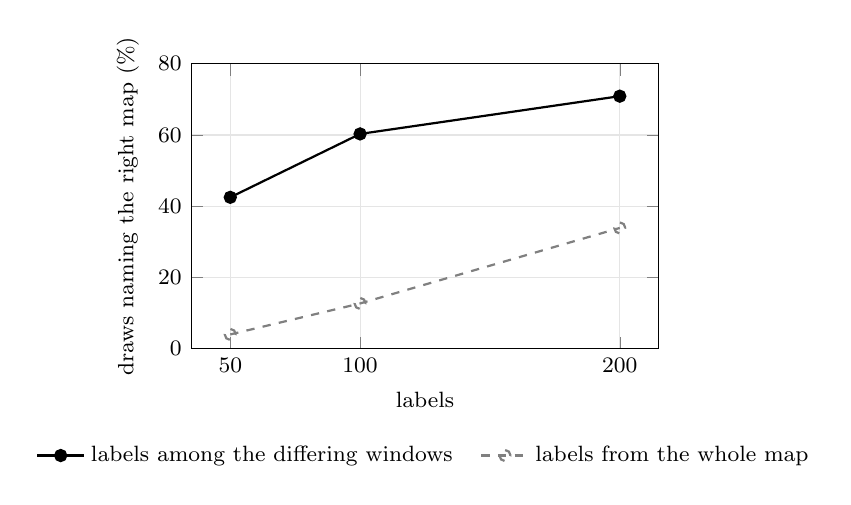
\begin{tikzpicture}
\begin{axis}[width=0.62\linewidth, height=5.2cm, xlabel={labels}, ylabel={draws naming the right map (\%)},
  xtick={50,100,200}, ymin=0, ymax=80, legend columns=2,
  legend style={font=\footnotesize, draw=none, at={(0.5,-0.3)}, anchor=north, /tikz/every even column/.append style={column sep=8pt}},
  tick label style={font=\footnotesize}, label style={font=\footnotesize}, grid=major, grid style={gray!20}]
\addplot[mark=*, thick, black] coordinates {(50,42.5) (100,60.3) (200,70.9)};
\addlegendentry{labels among the differing windows}
\addplot[mark=o, thick, gray, dashed] coordinates {(50,4.0) (100,12.7) (200,33.9)};
\addlegendentry{labels from the whole map}
\end{axis}
\end{tikzpicture}
\caption{exp90, means over 2,514 pairs of encoder maps: how often the 95\% interval on the accuracy difference excluded
0 on the right side. Both curves use the same interval; the whole-map labels are analysed on the differing windows
they hold. At 200 labels the whole-map draw labels the entire map on the 268 pairs of the three 200-unit AWF tasks.
\claim{exp90-which-map-few-labels}}
\label{fig:whichmap}
\end{figure}

\subsection{Published products against an independent probability sample}
\label{sec:res-products}

exp92 graded two labelled routes, the error-rate interval and the comparison of two maps, and the ranking on published
products; the certified zone was not graded. The reference is LCMAP's Reference Data Product v1.2
\citep{pengra2020}: 25,000 plots, a simple random sample of the 30\,m pixels of the conterminous United States,
interpreted into LCMAP's eight classes; for 2018 the maps are LCMAP Collection 1.3 primary land cover with its
confidence, and Esri's 10\,m Annual Land Use Land Cover v2 crosswalked to LCMAP's classes. The 24,968 plots where the
reference and both maps have a class stand in for the map population, so every design is graded exactly against
their truth. All four preregistered predictions held. LCMAP is 82.3\% and Esri 79.6\% accurate against this reference,
and the maps differ on 21.6\% of plots. Labels drawn among the differing plots covered the 2.7-point difference on
98.5\% to 99.0\% of 2,000 draws at 50, 100 and 200 labels, at about half the width of labels drawn from all plots, and
never named Esri; at so small a difference they named LCMAP on 12.0\% of draws at 100 labels (2.5\% from all plots).
Three hundred random plots gave an exact error-rate interval that covered on 95.0\% and 95.65\% of draws
\claim{exp92-products-labelled-routes-hold}. LCMAP's own confidence ranked its errors with an AUROC of 0.753 (bootstrap
interval 0.734 to 0.771), and its 10\% least confident plots held 28.7\% of the errors
\claim{exp92-lcmap-confidence-ranks-its-errors}. After the result, the comparison was found to need about 800 labels to
name LCMAP on 95\% of draws, against more than 3,200 for labels drawn from all plots. A pre-record audit found that
the first extraction had left out 734 plots with Esri data; the numbers here are corrected, with the same verdicts.
The reference uses LCMAP's legend, so Esri is graded through a crosswalk at a finer resolution, and the difference
measures agreement with this reference rather than which product is better in general. Whether any reference plot
was used to train LCMAP Collection 1.3 was not checked; the evidence is one year in one country.

Five more reference samples from four sources extend this (exp94, preregistered): NLCD's 2011 and 2016
accuracy-assessment points (stratified, the United States, 2001 to 2016), JRC's GFC2020 validation set (stratified,
global forest, 2020), the East Africa TimeSync sample (random within seven countries, 2015 to 2017) and the S2GLC
validation set (Europe, 2017, not a probability sample), graded against seven products: NLCD against LCMAP, GFC2020
against ESA WorldCover, CGLS-LC100 against Esri, ODSE-LULC against Esri. The points stand in for the map, as above.
Labels drawn where two products differ covered the difference on 98.05\% to 99.25\% of draws in all eight pairs, at a
third to two thirds of the width of labels from all points, and named the worse-agreeing product on at most 0.35\%;
on the four pairs differing by 4 to 6 points, 200 such labels named the better-agreeing one on 83\% to 95\% of
draws, against 13\% to 25\% from all points. The exact error-rate interval covered on 95.05\% to 96.25\% of draws in
all 18 cells \claim{exp94-labelled-routes-hold-on-four-references}. LCMAP's, CGLS-LC100's and ODSE-LULC's own
confidences ranked their errors, AUROC 0.720 to 0.787 in nine cells, every bootstrap lower end at least 0.704
\claim{exp94-product-confidences-rank-their-errors}. A pre-record audit recomputed 346 quantities by independent code
and changed none. Several pairs are related: LCMAP was trained on NLCD's 2001 map, and GFC2020 is built partly from
WorldCover (their errors correlate at 0.51); ODSE has no class over the sea, and CGLS no probability for water or
built-up land, so those points are outside the gradings.

exp106 asked whether a second opinion from another product, Esri's 10\,m land cover, flags three of these products'
confident errors (confidence at or above the median of their correct rows) and improves their review order, putting
the disputed rows first (preregistered; every row weighted equally). The order gained at least 0.02 of AUROC on 2 of 3
cells, ODSE (+0.077) and LCMAP (+0.079), against $-0.002$ on CGLS; the LCMAP cell is not blind, exp92 having graded both
scores on its rows, and 0.035 of its gain is tie-breaking in lcpconf \claim{exp106-second-opinion-order-gains-on-two-of-three}.
The flag marked confident errors 4.11 and 4.96 times as often as confident correct rows on ODSE and LCMAP and 1.45 times
on CGLS, so the preregistered twofold on all three did not hold; Esri repeats 69.3\% of CGLS's confident errors, and
most flagged confident rows are correct (10.0\% to 27.9\% are errors)
\claim{exp106-second-opinion-flags-confident-errors-on-two-of-three}. A related product, NLCD for LCMAP, meets the
ratio too, so it does not measure independence \claim{exp106-a-related-second-product-also-meets-the-ratio}.

\subsection{Two agencies' stratified samples: NLCD 2016 and GFC2020}
\label{sec:res-agency}

exp117 (not preregistered) built \code{grade} (Section~\ref{sec:agency}) and graded it on two of exp94's samples by
their agencies' designs: NLCD 2016's assessment \citep{wickham2021}, set B, 4,629 points in 21 strata, and GFC2020's
validation set \citep{colditz2025,bourgoin2026}, 21,612 points in 149 strata given as areas. In its design study the
dynamic programme matched every order of the labels to $3.6\times10^{-15}$, the expected e-value at the truth was at
most 1.000000000000001, a judge's 14 enumerated cells at $\alpha$ 0.1 and 0.3 held for every form claimed valid (least
slack 0.076) where normal theory covered as little as 0, and in a simulation at the designs' shapes (300 draws, 8
cases) the valid intervals covered 0.997 to 1.000 and normal theory 0.937 to 0.970
\claim{exp117-intervals-hold-exactly-and-in-simulation}. The selection rule fixed in advance chose a boxed stratified
Chernoff fallback because three of its gates could not be evaluated in time; the betting interval (a median 0.91 of the
fallback's width, 0.55 to 1.10) and the box (0.98 of the fallback's, and 1.27 of a certified scan of the ratio that took
up to 2,327\,s where the box took about 6\,s) were chosen afterwards, on widths \claim{exp117-design-study-widths}.

Run end to end, \code{grade} 1.18.0 reproduces NLCD 2016's published overall accuracies: 86.39\% by the
primary-or-alternate rule (published 86.4\%), 72.11\% by the primary label (72.1\%), 86.51\% for 2011 (86.5\%) and
78.99\% at level~I (79.0\%); level~I with the alternate is 90.70\% against 90.6\%, and GFC2020 V2 is 91.51\% accurate
(published as 91.5\%, 91\% in the abstract) \claim{exp117-grade-reproduces-published-overall-accuracies}. On all 10
overall accuracies and differences the valid interval is 1.60 to 1.64 times as wide as normal theory's, and every
printed interval equals the design study's own (largest difference 0.0)
\claim{exp117-valid-interval-costs-1-6-times-normal}; for NLCD 2016 the two are 84.11\% to 88.40\% and 85.07\% to
87.71\% (\code{exp/out/exp117\_summary.json}). NLCD leads LCMAP at eight classes by 1.34 points, 0.41 to 2.26
by normal theory and $-0.17$ to 2.86 by the valid interval. Normal theory is not wrong there: it covered that
difference on 0.948 of 5,000 draws at NLCD's shape (exp118) \claim{exp118-normal-theory-short-on-classes-not-overall},
so the disagreement is the valid interval's width
\claim{exp117-normal-theory-calls-a-difference-the-valid-interval-does-not}. For all 15 NLCD classes the pure-stratum
rule's user's-accuracy interval is narrower than the box, a median 0.61 of its width (0.32 to 0.76) and 1.20 to 3.87
times normal theory's (median 1.43); class 21 gets 79.4\% to 91.8\% where the box gives 69.9\% to 100\%
\claim{exp117-pure-stratum-rule-narrower-than-box}. A class with few labels can get a producer's accuracy of 0 to
100\% (NLCD's class 24, 0.26\% of the reference).

NLCD's per-class table (Table~4 of \citealp{wickham2021}) was reconciled after 1.18.0. It was transcribed correctly,
and by the primary label all 15 user's and 15 producer's accuracies are reproduced (largest gap 0.47 points). The
table's primary-or-alternate user's accuracies are reproduced, all 15, only when the 2011 primary label is also
accepted, a rule the paper does not state; that gives 86.955\% overall, which the caption of Table~4 in the published
version prints, truncated, as 86.9\% where the text and Table~1 give 86.4\%. No rule tried
reproduces its producer's accuracies (the best matches 7 of 15, 4.40 points off at class 95). Since 1.18.1
\code{-{}-alternate} takes several columns, and with the 2011 primary label as one of them \code{grade} gives the same
15 user's accuracies \claim{exp117-nlcd-table4-reconciled}.

exp118 (preregistered, frozen at 000bdf7) checked \code{grade} twice. A second implementation written from the plan
alone, without the package or the design study's scripts, reproduced every interval of the five exp117 runs its plan
named (NLCD 2016 level~II by both rules, 2011, NLCD against LCMAP, and GFC2020), within
$1.2\times10^{-14}$ for linear quantities and differences, $6.7\times10^{-13}$ for boxes and $1.1\times10^{-7}$ for the
pure-stratum rule (bar $10^{-6}$) \claim{exp118-second-route-reproduces-grade}. On populations of ten copies of each
NLCD 2016 stratum's points, over 5,000 draws without replacement graded by 1.18.1 from PyPI, the valid interval covered
at least the bar of 0.9408 (0.95 less three Monte Carlo standard errors) on all 91 quantities, the least 0.9826 \claim{exp118-valid-intervals-hold-at-nlcd-shape}.
Normal theory fell below the bar on 33 of the 91, all per class: 16 of 29 producer's accuracies (least 0.835), 9 of 29
reference shares and 8 of 29 user's accuracies (least 0.712, LCMAP's water at eight classes); on the overall
accuracies and the difference it covered 0.948 to 0.951 \claim{exp118-normal-theory-short-on-classes-not-overall}. The
valid intervals' mean width over normal theory's was 1.62 to 1.63 for overall accuracy, with medians of 1.90 for user's
accuracy (1.19 to 4.17) and 2.40 for producer's (1.99 to 5.65) \claim{exp118-valid-interval-width-cost}. The plan's
GFC2020 arm was cancelled for its compute cost before any of its results was read, so GFC2020's coverage was not
measured, and the copied populations hold the samples' shares and make each draw closer to a census than the agency's.

What 1.20.0's new intervals cost was measured as release checks, descriptive and not preregistered (exp119). On the
demo tile, \code{estimate -{}-valid}'s interval was 1.72 and 1.64 times as wide as the confidence design's Wilson
interval at 300 and 1,000 labels, and 0.60 times as wide as the class design's union bound at 1,000 labels, where it is
both narrower and valid; on one core the whole-map interval took at most 0.27~s and the per-class ones at most 1.05~s
\claim{exp119-valid-interval-cost-on-the-demo-tile}. On NLCD 2016's eight-class two-map grade, the 26 direct ratio
intervals of \code{grade -{}-ratio direct} took 627~s in all on one core (446~s at a tolerance of $10^{-4}$), each a
median 0.82 of the box's width (0.64 to 0.92) and a median 1.73 times normal theory's (1.62 to 3.56)
\claim{exp119-ratio-direct-cost-on-nlcd}. GFC2020's direct intervals lie above the work bound, so \code{grade} gives
the box there, and the box stays the default.

\subsection{Another organisation's deployed field map}
\label{sec:res-ftw}

exp110 (preregistered, frozen before any metric was computed) is the record's first test on another organisation's
deployed product outside land cover: FTW's 2nd-edition global field map, whose per-pixel field and boundary
probabilities come from FTW's ftw-q model, read by the package as a two-class field-extent probability (field plus
boundary) at the FTW benchmark v1 test chips of Belgium, Croatia, Slovenia and Sweden: 1,295 chips, 1,321,132
windows of $8\times8$ mask pixels with a truth majority, graded against the benchmark's masks from parcel declarations,
photo-interpreted parcels and LPIS blocks, taken as right. The benchmark's 2-class mask turned out to be field only,
its boundary pixels coded background; as the owner ruled after the run, the graded result keeps the preregistered
truth, and the field-plus-boundary reading is reported beside it. The map's confidence ranked its window errors at
AUROC 0.837, 0.870, 0.936 and 0.863, the least confident 10\% holding 0.308 to 0.694 of them, and led the best
no-model control by 0.127, 0.098 and 0.307 in Croatia, Slovenia and Sweden but by 0.018 in Belgium (90\% chip
bootstrap 0.004 to 0.034, against the rarity of the predicted class), so the ranking prediction held in 3 of 4
countries \claim{exp110-ftw-map-confidence-ranks-its-window-errors}. The three checks held: the exact interval covered
with probability at least 0.957 in all ten cells, certify's zone was wrong more often than $\alpha = 0.05$ on at most
4.0\% of 2,000 draws, and labels drawn where two maps differ named the worse-agreeing one with probability at most
0.0036 \claim{exp110-ftw-labelled-routes-keep-their-guarantees}. At 300 labels the median certified share was 0.40,
0.45, 0.90 and 0 (Sweden), a quarter or more in 3 of 4 against a preregistered at least 2 of 4, but fragile: each country certifies any zone
with an exact probability of 0.484 to 0.525, so each median sits on that edge, and 22\% to 51\% of the windows sit at
confidence exactly 1, where the package's tie rule (raster order), not evidence, decides which enter a zone
\claim{exp110-ftw-certified-share-at-300-labels}. exp112 later found that this budget is where the first level enters: any
map certifies with probability at most about 0.525 there, so the verdict turned on whether each country's most confident
15\% was almost free of errors. With 100 labels drawn where the map and FTW's PRUE B3 model, run by
the record on the benchmark's imagery, differ, the better-agreeing map was named with probability 0.858 (Belgium, B3),
0.999 (Croatia, the 2nd-edition map) and 0.993 (Sweden, B3), as predicted for 3 of 4, but not in Slovenia (0.141) or
pooled (0.063); B3 most likely trained on these countries' train chips too, so this says which map agrees better on
these test chips, not which generalises better \claim{exp110-ftw-which-map-at-100-labels}. Under the field-plus-boundary
truth the pooled window error rate is 0.1025 against 0.1110, lower in three countries and higher in Sweden, so the
boundary pixels account for only part of the errors, and the six verdicts are the same
\claim{exp110-ftw-field-plus-boundary-reading}. The run script was untracked when it ran; its recorded sha256 matches
the committed file, and an independent recomputation with its own code reproduced every graded number.

\subsection{A blind transfer test}
\label{sec:res-blind}

exp111 (preregistered, frozen before any prediction at a fresh plot) asks whether exp99's ranking miss under transfer
and exp109's diagnosis of it hold where no model has looked: 900 Kenya and Tanzania TimeSync 2017 plots more than
100 km from the AWF area, drawn 300 Open Grassland, 300 Wooded Grassland and 300 other (890 with input), read from
rslearn 0.1.17 directly after a known-answer gate at the points exp98, exp99 and exp103 graded. The record's v1.2
fine-tune passed the gate (259 of 259 and 262 of 263 the same class as its earlier runs); Ai2's v1 did not (245 of
259, 237 of 263), under any route the record tried, so by an amendment made after the gate and before any blind
prediction v1.2 is graded and v1 reported beside \claim{exp111-v1-does-not-reproduce-exp98-under-rslearn-0117}.
The confidence ranked the STRICT errors at a region AUROC of 0.729 (90\% bootstrap 0.701 to 0.758), above the 0.70
bar exp99 missed, so the predicted miss did not replicate; the lower end sits at 0.70, so the AUROC is not shown to
be above the bar either \claim{exp111-v12-ranking-reaches-the-bar-at-fresh-plots}. Standardised to exp99's label
mix, as preregistered, the grass/shrub definitional pair was 0.611 of the confident STRICT errors (interval 0.438 to 0.768;
13 of 25 unweighted), as exp109 diagnosed; weighted by region it is 0.334, and the map's montane forest class
holds the largest region-weighted share of the confident STRICT-only errors (0.469), so the diagnosis holds
standardised and unweighted, not region-weighted
\claim{exp111-v12-grass-shrub-pair-is-most-confident-strict-errors}. The confidence was not blind to the STRICT-only
errors (0.656 against the predicted at most 0.65) \claim{exp111-v12-strict-only-errors-rank-just-above-the-bar}, and a 20-label
per-class audit would flag the pair with probability 0.287, not more often than not
\claim{exp111-v12-twenty-label-audit-does-not-reliably-flag-the-pair}. An independent recomputation from the frozen
page reproduced every graded number.

\subsection{A map made from OlmoEarth v1.3 embeddings}
\label{sec:res-v13}

exp112 (preregistered, frozen before any statistic of the map) grades a map made the way Ai2's OlmoEarth v1.3 invites:
a default logistic regression fitted on the 2018 v1.3 embeddings (128 dimensions) of 1,000 random plots of LCMAP's
reference sample and applied to the other 11,000 plots of a 12,000-plot draw, a simple random sample of CONUS's 30 m
pixels that stands in for the map. The map errs on 11.7\% of the plots, and its top probability ranks those errors at
an AUROC of 0.876 (90\% bootstrap 0.869 to 0.884), the least confident 10\% holding 41.6\% of them; both no-model
controls are near chance, so the lead of 0.366 mostly measures the AUROC's distance from 0.5
\claim{exp112-v13-map-confidence-ranks-its-errors}. The exact interval, the certified zone's guarantee and the
which-map route held \claim{exp112-labelled-routes-keep-their-guarantees}. The preregistered certified share failed:
at 300 labels and $\alpha = 0.05$ the first level the cut tests expects exactly the 45 labels it needs, so any map
certifies with probability at most 0.525, and the bar passes only a map with at most one error among its most confident
15\%; this one has two, a limit found after the run that exp110's bar shared
\claim{exp112-p3b-fails-at-the-level-cut}. The map agrees with the reference more often than LCMAP Collection 1.3 and
Esri do, but it was fitted on that reference's plots, so this is agreement with its conventions, not accuracy
\claim{exp112-agreement-with-the-reference-not-accuracy}. The fit points were spread at random over the same
population, the favourable case; the next subsection grades a regional fit. An independent route refitted the map and
reproduced every graded number.

\subsection{A regional map from embeddings: PLANTEUR}
\label{sec:res-planteur}

exp113 (preregistered, frozen before any label or embedding was read) grades the regional case on Ai2's PLANTEUR
crop-type benchmark: patches in France's overseas territories labelled from the parcel registry, with 2019 embeddings
from OlmoEarth v1.3, TESSERA v2 and AlphaEarth on the label grid. For each of five territories a default logistic
regression was fitted on 100,000 random pixels of the other territories and applied to the held-out one, graded on
4 by 4 pixel windows. v1.3's confidence ranked the held-out map's errors at AUROC 0.874, 0.857, 0.816, 0.876 and 0.742,
meeting the preregistered bars in 5 of 5; the lead over the best no-model control is informative in three of them,
where a boundary or distance control ranks errors on its own \claim{exp113-v13-ranking-holds-on-held-out-territories}.
The prediction that transfer costs at least 0.05 of AUROC failed narrowly: the mean drop against the default split is
0.047, from 0.004 to 0.138 by territory \claim{exp113-transfer-drop-in-ranking-below-the-bar}. The interval, the
certified zone at 400 labels and the which-map route kept their guarantees at all 18 maps
\claim{exp113-labelled-routes-keep-their-guarantees}. In three territories the held-out map is close to an
all-Background map, so there the confidence mostly finds registry crop land the map calls Background; in the other two
it classifies crops \claim{exp113-held-out-maps-mostly-background}. The best-agreeing embedding was v1.3 in four
territories and TESSERA v2 in one, mostly by small gaps \claim{exp113-which-embedding-agrees-best}. An independent
route drew the same fit pixels and reached the same verdicts.

\subsection{Why the held-out maps collapsed, and an exact per-class report}
\label{sec:res-pathway}

Bayes' rule splits a classifier's posterior into a likelihood and a prior, so a map fails on new ground through a change
in the class shares, which reweighting repairs, or through a change in a class's features or calibration, which it does
not. exp114 (preregistered) refitted exp113's maps, identical on every window, and corrected them with the true class
shares: the v1.3 maps' mean posterior still missed those shares by 0.089 in Guyane and 0.198 in Réunion, against 0.009
on the default split, so most of those failures are not a change of class shares, while Mayotte, whose crops are 0.6\%
of the land, is not determined \claim{exp114-prior-correction-leaves-the-gap}. EM's label-free estimate of the shares
was closer to the truth than the maps' own shares in 3 of 15 held-out maps against a predicted 10
\claim{exp114-label-free-priors-mislead-under-feature-shift}. An exact test from 400 random pixel labels rejected it with
probability 1.000 on every held-out v1.3 map while rejecting the true shares at most 2.3\% of the time; it also rejected
it in-distribution, where EM was close, so a rejection says the label-free shares are not to be trusted, not which
pathway failed \claim{exp114-random-labels-catch-a-wrong-prior-estimate}. exp115 (preregistered) graded a per-class
report in which every interval is exact, each class's share by a hypergeometric interval and its producer's accuracy
bounded by the map's own count of the class, with probabilities summed over every possible sample on 39 fully labelled
maps: every guarantee held \claim{exp115-exact-per-class-guarantees-hold}. Of 17 classes with a share of at least 5\%
drawn at half of it or less, 400 labels flagged 16 with probability at least 0.8, and of 10 such classes with producer's
accuracy at most 0.10 they bounded 9 at 0.25; each prediction missed by one class, and classes under 1\% of a map were
rarely flagged \claim{exp115-flag-and-bound-show-a-collapsed-class}. The predicted quiet on classes within 0.02 of their
share failed: the flag's power follows the gap in sampling errors, so it is not to be printed without its interval
\claim{exp115-flag-on-near-right-classes}. Independent routes reproduced every graded number of both.

\subsection{Estimation from a labelled sample}
\label{sec:res-estimate}
\label{sec:est-results}

exp116 (preregistered) graded the class design on 269 of the suite's unit maps, 400 labels and 400 draws each: every
class's user's accuracy covered on at least 0.917 of draws for 2,401 of 2,402 (map, class) pairs, the one below at
0.9125 having an exact coverage of 0.954, and the class areas with the producer's accuracies, and the overall
accuracy, held together on every map (smallest 0.9775) \claim{exp116-class-design-exact-intervals-hold}; for all
1,148 classes under 5\% of their map the class design's user's-accuracy interval was narrower than a random sample's
of the same size, a median 0.61 of its width \claim{exp116-class-design-narrows-rare-classes}. The run read 24 files
outside the plan (a second run of one encoder); on all 380 every prediction holds too, and an independent route written
from the plan alone reproduces every map of the planned files exactly.

exp78 graded the estimators on the suite's seven segmentation tasks, from an export that reproduces exp70's
accuracies \claim{exp78-export-reproduces-the-suite}. With 300 randomly sampled windows the finite-population Wilson
interval, the form the package printed at the time, covers the true error rate on 0.933 to 0.961 of 2,000 draws on all
seven \claim{design-based-interval-is-honest}, with a half-width of about 3 points at a low error rate and 5 at a high
one; on all sixteen encoders it covers 0.933 to 0.963, and the exact interval the package now prints has an exact
coverage of at least 0.9506 on the same 111 cells \claim{exp79-estimation-findings-hold-on-every-encoder}. Taken as
18 tiles of 16 windows with the independent-sample formula, the interval covers on 0.506 to 0.777 of draws on six of
seven tasks; the ratio estimator covers 0.913 to 0.932 on the four tasks with full tiles, 0.824 on Sen1Floods11 and
0.598 on MADOS, whose tiles hold 1 to 400 windows \claim{tile-sampling-breaks-the-naive-interval}. The tile design as
the package ships it, checked without preregistration, covers 94.5\% to 95.4\% on five tasks and falls short on Sen1Floods11 (84.3\%) and MADOS (68.5\%), the two tasks where a tenth of the
tiles hold most of the errors \claim{shipped-tile-design-coverage}. The confidence design narrows the interval to a
median 0.80 of the random width with coverage intact, but its clause requiring a ratio above 0.94 at over 30\% error
failed at 0.9361 \claim{confidence-helps-most-where-the-map-is-good}; it saves up to 2.51 times the labels, above the
preregistered 1.8 \claim{confidence-saves-a-quarter-to-a-half-of-the-labels}. Against the practitioner's design,
strata by the map's classes with proportional allocation and the stratified estimator \citep{olofsson2014}, the
shipped confidence design (exp105, preregistered, on exp78's 24 exports at 2,000 draws) gives a valid and no wider
interval for the overall rate on 14 of the 18 tasks gradable at 300 labels, the preregistered bar, at a median 0.853 of
the width; both cover on every task, and the four losses are 1.5\% to 2.6\% wider. The count turns on the coverage
rule at m-brick-kiln (0.941 in this run, about 0.934 over 30 reruns at other seeds, 7 of which gave 13)
\claim{exp105-confidence-design-narrower-than-map-class-strata}. Map-class strata given the same allocation rule lose on
16 of 18, so the gain is the strata's \claim{exp105-the-gain-is-from-the-strata}; for the overall rate map-class
strata gain little over a random sample, as Cochran's formula predicts. At 100 labels on a 200-window map the
confidence design covered 0.913 \claim{exp105-confidence-design-short-at-100-labels-on-200-windows}. Labelling the 5\% review set and dividing
gives 1.8 to 5.8 times the true rate on the seven tasks (from exp70's capture at 5\%), the case the review-set check
refuses.

Each condition's exact interval, applied to a random sample of 300 windows split by condition, was graded on exp88's
half-cloudy map above, covering 95.6\% and 95.7\% \claim{pooled-error-rate-misstates-the-cloudy-part}; the condition
design's equal allocation and its whole-map union-bound interval were not. The whole-map union-bound interval, the \code{?} interval,
the reviewer-error interval, the per-condition certificate and the interval on the difference of two maps are checked
by exact enumeration on populations of 10 to 100 windows in the test suite, where each keeps its stated guarantee against
every error pattern (the per-condition certificate against five patterns per condition on every draw), every
adversarial choice of unjudged windows and every reviewer within the stated rates. Apart from the per-condition
intervals above and exp90, none of them has been graded on a real map in a recorded experiment.

For per-class accuracy (exp81), the Wald interval of the map-accuracy literature leaves 107 of 522 cells below 0.93
coverage, the worst at 0.019, as it collapses to a point when a class shows no sampled error; the package's forms leave
14 of 628, none below 0.879, and no random-design user's-accuracy cell below 0.947
\claim{per-class-intervals-wald-fails-wilson-nearly-holds}. On the nine rare-error cells the few-errors warning fires
on 1,081 of the 1,351 draws whose interval misses \claim{rare-error-warning-marks-the-misses}, and the confidence design's per-class
user's-accuracy intervals at 300 labels are narrower than a random sample's on 19 of 21 tasks
\claim{confidence-design-serves-the-classes-too}.
exp85 measured a model-assisted difference estimator with a tuned coefficient (PPI++; \citealp{angelopoulos2023ppipp}). Under a random sample it covers 0.94 to 0.95 at 0.840 to 0.930 of the Wald width
\claim{model-assisted-arm-is-honest-and-never-wider}; under the confidence design its stratified form \citep{fisch2024} saves 3.5\% to 5.4\% of labels at 0.4 to 1.0 points of coverage, and by the preregistered rule it was not adopted
\claim{model-assisted-gain-beyond-the-design-is-two-percent}.

\subsection{The certified zone}
\label{sec:zone-results}

On OlmoEarth Base's 24 tasks at 100, 300 and 1,000 random labels with $\delta = 0.1$ (exp80), the prefix zone exceeded
$\alpha$ on at most 0.080 of 2,000 draws and the Bonferroni zone on at most 0.0045, on all 112 cells (110 with a
testable level), against a bound of 0.120; the plug-in zone, the largest with a sample error rate of at most $\alpha$, exceeded it on up to 0.557
\claim{trust-zone-guarantee-holds}. At 300 labels and $\alpha$ half the error rate, the plug-in exceeds $\alpha$ on more
than $\delta$ of draws on 16 of 21 tasks \claim{plugin-zone-violates-on-most-tasks}, and the prefix rule certifies a
zone on most draws on 14 of the 21 tasks, its median certified coverage 0.50 against an oracle median of 0.60
\claim{trust-zone-coverage-at-300-labels}. The guarantee held on four other encoders too
\claim{trust-zone-guarantee-holds-on-other-encoders}. On a published product's own confidence (exp93: LCMAP Collection
1.3's \code{lcpconf}, against the 4,796 plots of exp92's confidence subset standing in for the map, 17.7\% wrong), the
prefix zone exceeded $\alpha$ on at most 6.1\% of draws and the Bonferroni zone on at most 0.2\% in all 24
rule-grid-cells, and the plug-in on 46.6\% at 300 labels and $\alpha$ half the error rate; there the prefix rule
returned no zone on 87.45\% of draws, as summed exactly before the run: the first level tested, a tenth of the plots
(those at 100 and a random part of the tie at 99), is 6.0\% wrong against $\alpha = 8.86\%$ and holds about 30
labels \claim{exp93-zone-guarantee-holds-on-a-product}. LCMAP's confidence is coarse, 55\% of the plots at 99. At
$\alpha = 8.86\%$ the prefix rule returned a zone more often on the product's own thresholds, \code{lcpconf} $\geq 99$
(57.6\% of those plots, 7.2\% wrong) or more on 25\% of draws at 300 labels and 60\% at 1,000, than on the package's
grid (13\% and 39\%); Bonferroni, and the prefix rule at $\alpha = 5\%$, went the other way (descriptive)
\claim{exp93-grid-choice-changes-what-is-certified}. Plots whose \code{lcpconf} is a provenance code (4\%, 29\% wrong) are
outside the zone's population and must be masked before certifying. On three products' confidences against
exp94's references, at 300 labels and $\alpha$ half the error rate (5.2\% to 20.9\%), the prefix zone exceeded $\alpha$
on at most 2.8\% of draws and the Bonferroni zone on at most 0.4\%, the plug-in on 39\% to 53\%, and the prefix rule
returned no zone on 73\% to 97\% of draws \claim{exp94-zone-guarantee-holds-on-three-products}. The mean top-1 probability exceeds accuracy by a median 0.061
\claim{mean-confidence-overstates-accuracy}, which is why the zone is calibrated on labels.

The guarantee is per budget, not per look. On nested samples, a larger budget adding labels to a smaller one, the
prefix rule's mean certified coverage fell by more than 0.05 of the map when labels were added on 14 of 34 maps
(exp95, preregistered; a level enters at the budget where it expects the minimum number of labels and must then be
passed with about that many), and a cut that tests a level later halved those falls but certified less at about 100
labels on 24 of the 34, so the standard cut stayed \claim{exp95-standard-cut-falls-when-labels-are-added}; a second
cut designed after exp95 passed at its preregistered seed on 332 other maps and not across seeds, and is an option,
not the default \claim{exp96-ramp-passed-at-its-seed-and-not-across-seeds}. Certifying at every budget of a doubling
ladder on six of those maps, where one budget's zone was wrong more than $\alpha$ on at most 12.25\% of draws, gave a
wrong zone at some look on 21\% to 30\% \claim{certify-guarantee-is-per-budget-not-per-look}. exp97 (preregistered)
graded the sequential certificate on the 366 maps: over 3,122 violation rates the largest was 0.1175 at $\delta = 0.1$
(bound 0.175, none above three standard errors), and its zone never shrank
\claim{exp97-sequential-certificate-holds-at-every-look}, where \code{certify} rerun after every 5\% more labels, a
median 77 looks, certified a wrong zone at some look more than 17.5\% of the time on 132 maps, at most 0.435
\claim{exp97-rerunning-certify-breaks-its-guarantee}. It costs labels: with the anchor of a first budget of 300, a
median 1.71 times the one-look rule's labels to reach half the largest mean certified share that rule reaches (213
maps), and over budgets 50 to 3,000 a median mean certified share of 0.146 against 0.222 on the same 279 maps
\claim{exp97-sequential-certificate-costs-labels}. The default stays the one-look certificate; the sequential one is
for a reviewer who will look more than once.

exp116 (preregistered) graded the target rule on 420 cells of the suite's unit maps per target (0.25, 0.5, 0.75),
with $\alpha$ half each map's error rate, $\delta = 0.1$ and 300 or 1,000 random labels: its zone was wrong more than
$\alpha$ on at most 0.0925 of 400 draws at target 0.5 and 0.095 at 0.25, against a bar of 0.145, where prefix reached
0.095 and Bonferroni 0.0125 on the same draws \claim{exp116-target-rule-valid-on-real-maps}. On the 771 cells where the
target zone is wrong at most $\alpha$, it certified at least the target on at least as many draws as Bonferroni
certified that level on 744 (0.965), on average 0.68 of draws against 0.41 at target 0.5
\claim{exp116-target-rule-certifies-its-target-more-often}. Read after the run, on 46 of the 413 cells where the target
rule at 0.5 certified a zone on some draw, more than $\delta$ of the zones it certified were wrong, though no cell's
share of all draws passed the bar \claim{exp116-issued-certificates-can-fail-more-often-than-delta}: $\delta$ is not
the chance that an issued certificate is wrong. On the package's Dynamic World tile at $\alpha = 0.10$, five random
samples with a 0.5 target certified zones 5.5\% to 8.1\% wrong against the expert labels and each certificate verified;
a class-design sample of 600 labels over nine classes certified nothing, so the preregistered ``all six'' does not hold
\claim{exp116-certificates-on-a-real-tile}.

\subsection{Use by a language-model agent}

exp64 preregistered whether the package helps an agent, on forty cards with hidden labels, using
\code{nvidia/Qwen3.8-27B-NVFP4}. With the package as tools, the model reproduced the review set, grounded 99.4\% of its
numbers and declined to choose a side on every comparison card \claim{agent-benchmark-tool-arm-reproduces-the-package}.
Two predictions failed. A numpy sandbox captured 0.904 of the package's errors
\claim{agent-benchmark-sandbox-rediscovers-the-ranking} and grounded 94.2\% of its numbers against 99.4\%, a gap below the
preregistered 0.2 once a grading that read only JSON fields was withdrawn \claim{agent-benchmark-grounding-not-decisive}.
The tool arm's decline held as graded, but an arm with only the card's text, no data and no package, also declined on
30 of 30 runs, so the benchmark cannot show that the package causes the decline \claim{agent-benchmark-decline-holds}.
At 7B all three predictions held \claim{agent-benchmark-package-is-a-floor-at-7b}, and the shipped agent called the
review-set tool on 17 of 40 runs against 40 of 40 at 27B \claim{agent-benchmark-7b-agent-does-not-find-the-tool}.

Two later agent results carry no ledger claim and are stated with their limits. In the OlmoEarth Agent trial exp86,
material false statements per sentence fell from 7.5\% to 2.2\% over development rounds 7 to 10, on the eight briefs
the fixes were built against; the trial passed only under an instrument amended fourteen times after results were
seen, and under the preregistered instrument its answers fail three of its predictions. The held-out trial exp87 has
been run and audited but not graded. Both trials' files are archived at tag v1.9.0 (Section~\ref{sec:avail}). In a pilot of 2 October 2026, agents answered five questions through the MCP
server on the outputs of the two fine-tuned models of Section~\ref{sec:res-finetuned}: the tools' numbers were right,
a strong model's replies kept the numbers and their limits, and a small model's replies failed on all five, mostly by
dropping limits; after the server's texts put each tool's main limit inside its conclusion, two of the small model's
five replies passed. The pilot was not preregistered and left no committed artifact; \code{estimate} and \code{certify}
refuse a review set, so a weak model's advice to label one cannot become a wrong number, though the reply can still
mislead.

\subsection{Conditions for reading a ranking}

On LUCAS, a probe that memorised its fit set placed the margin last of four model signals and a regularised probe
placed it first \claim{lucas-overfitting-inverts-the-ranker-ordering}; on the suite the effect has the same direction at
a magnitude of four ten-thousandths \claim{suite-probe-gap-degrades-the-ordering}. A ranking comparison should therefore
be reported with the probe's generalisation gap. Filtering a reference to large homogeneous units favours the ranking
(AUROC 0.774 on the kept LUCAS units, 0.677 on the deleted ones) \claim{lucas-the-homogeneity-filter-flatters-the-tool}.

\section{Contributions and practice baselines}
\label{sec:contrib}

No part of \pkg{} is claimed as a new statistical method. For each part, this section names what a practitioner would
otherwise do, what the record measured against it, and the comparisons it has not run. Except where a product, a
fine-tuned model or a deployed model is named, the maps below are the record's linear probes on frozen embeddings,
graded on benchmark splits that are not landscape samples.

\textbf{Review order.} Ranking outputs by the model's softmax confidence is the literature's baseline for finding
misclassified examples \citep{hendrycks2017,jaeger2023}, and the margin is the score of margin sampling
\citep{scheffer2001}. The package ranks by the margin, a close relative of that baseline, and does not improve on it:
one minus the top probability ranks errors slightly better than the margin on 14 of 16 multi-class suite tasks, by a
median 0.0006 of excess AURC \claim{top1-beats-the-margin-on-multiclass}. The record adds a replication across encoders
and seeds and tests of the alternatives. Across sixteen encoders, their tasks and ten probe seeds the margin beats a
random order in all 3,560 cells, the lowest AUROC 0.503, close to chance \claim{exp79-margin-beats-random-everywhere},
and on OlmoEarth Base it closes a median 0.68 of the gap between a random and a perfect order
\claim{margin-takes-two-thirds-of-the-ranking-headroom}; both are readings of the runs' outputs made afterwards, not
preregistered. A five-seed ensemble, which beat it on 2 of 24 tasks, and nearest-neighbour and Mahalanobis distances,
which beat it on none \claim{suite-margin-beats-the-strong-alternatives}, and the encoder-internal, perturbation and
typicality signals of Table~\ref{tab:neg}, on expert labels \claim{no-encoder-internal-signal-beats-confidence}, did not
improve on it overall; a fusion of five readings fitted to labels did, on two Sen1Floods11 testbeds
\claim{calibrate-ranker-fusion-beats-confidence}. The limits are part of the result. The suite's no-model controls are
near chance, a reading made after a red-team review and not preregistered, so the wins over them show little beyond a
win over a random order \claim{suite-controls-are-near-chance}.
On Sen1Floods11 Bolivia, one flood event, a water index that uses no model ranked the errors as well as the confidence
under OlmoEarth v1 and better under v1.2 \claim{bolivia-ndwi-exception}, and under a Sentinel-1 probe it ranked them
better on the whole multi-region test split \claim{s1-probe-ndwi-flip}. On one task, in runs that changed the year, the place, the
legend and the kind of point at once, the ranking missed its bar of 0.70 for Ai2's fine-tuned AWF model and for the
record's own fine-tune of that task on OlmoEarth v1.2 (AUROC 0.638 and 0.642 under the one-to-one crosswalk), and the
runs cannot say which change weakened it \claim{exp99-confidence-misses-the-ranking-bar-under-both-rules}
\claim{exp103-v12-transfer-ranking-misses-under-strict}; the second model shares the first's task, labels, region and
recipe, so it repeats the test rather than adding an independent one. A preregistered blind test at 890 fresh plots
of the same sample more than 100\,km from the area did not repeat the miss for the v1.2 fine-tune (0.729, interval
0.701 to 0.758, its lower end on the bar) \claim{exp111-v12-ranking-reaches-the-bar-at-fresh-plots}. At the same plots
as exp99, under the one-to-one crosswalk, a
perturbation step after confidence did not catch more errors \claim{exp101-shaking-does-not-help-under-transfer}.
Most of the confident errors at exp99's plots lie on one grass/shrub boundary that neither legend defines, which no label-free reading
in the record separates; the per-class audit of Section~\ref{sec:audit} can name such a class from labels but not its
windows \claim{exp109-transfer-confident-errors-lie-on-one-contested-pair}, and at the fresh plots 20 labels per class
would have named it with probability 0.287 \claim{exp111-v12-twenty-label-audit-does-not-reliably-flag-the-pair}. On a
second task under a smaller shift, months
after training inside the training region, the confidence of Ai2's Forest Loss Driver model ranked its disagreements
with analysts' labels at an AUROC of 0.770, at or above the bar of 0.70 on the point value, though the 90\% interval,
0.682 to 0.855, contains 0.70, so the run does not show the AUROC above the bar
\claim{exp104-forest-loss-confidence-ranks-the-disagreements}; it does not explain the first miss. No label-free reading
tried finds the errors a model makes confidently. Post hoc, the 18 confusions between exp104's two labelled classes rank
at an AUROC of 0.400, with a median top-1 probability of 0.995, as for the correct alerts, though with the labels taken
as right the run cannot say whether they are the model's errors or the reference's
\claim{exp104-the-ranked-disagreements-leave-the-two-labelled-classes}.

\textbf{Error rate.} Practice draws a simple random sample, or stratifies by the map's classes and uses the stratified
estimator \citep{olofsson2014}; stratifying an evaluation sample by a classifier's confidence was proposed by
\citet{kumar2016}. Against a simple random sample, on seven segmentation tasks, the confidence design narrows the
interval to a median 0.80 of the width with coverage intact, though its preregistered clause for maps over 30\% error
failed (a width ratio of 0.9361 against a bar above 0.94) \claim{confidence-helps-most-where-the-map-is-good}. Against
map-class strata with proportional allocation (exp105), on the 18 tasks gradable at 300 labels, it gives an interval
that covers at least 0.93 and is no wider on 14, the preregistered bar, at a median width ratio of 0.853 (bar 0.90); the
count turns on one task's coverage, and 7 of 30 reruns at other seeds gave 13, below the bar
\claim{exp105-confidence-design-narrower-than-map-class-strata}. Against map-class strata given the confidence design's
own allocation rule it wins on 16 (bar 12), so the gain comes from stratifying by confidence, not from the allocation
\claim{exp105-the-gain-is-from-the-strata}. Report-only, at 100 labels on a 200-window map the design covered 0.913
\claim{exp105-confidence-design-short-at-100-labels-on-200-windows}; its interval is nominal, with no finite-sample
guarantee. Map-class strata are built for class areas and per-class accuracy, which exp105 did not grade. A
model-assisted estimator added to the confidence design, the stratified form \citep{fisch2024} of PPI++
\citep{angelopoulos2023ppipp}, saved 3.5\% to 5.4\% of labels at a cost of 0.4 to 1.0 points of coverage and was not
adopted \claim{model-assisted-gain-beyond-the-design-is-two-percent}. The record also measured two practices that fail.
The Wald interval for per-class accuracy leaves 107 of 522 cells below 0.93 coverage, the worst at 0.019, against 14 of
628 for the package's forms, whose preregistered bar of every cell at 0.93 also failed
\claim{per-class-intervals-wald-fails-wilson-nearly-holds}. Labels collected by tile and treated as independent cover on
0.506 to 0.777 of draws on six of seven tasks \claim{tile-sampling-breaks-the-naive-interval}, and the package's own
tile design, checked without preregistration, falls short on two of the seven, at 84.3\% and 68.5\%
\claim{shipped-tile-design-coverage}.

\textbf{Which of two maps is more accurate.} Practice labels one shared sample and tests the paired outcomes with
McNemar's test \citep{foody2004}, which uses only the units where exactly one map is right; disagreement maps point
reviewers to where products differ \citep{fritz2008}. Drawing the labels where two maps differ follows the same logic,
since the windows where they agree carry no information on the difference. The record graded this design, without
preregistration, against labels drawn from the whole map and analysed with the same interval on the differing windows
they held: over 2,514 pairs of probe maps, 100 labels named the right map on 60.3\% of draws against 12.7\%, and on the
pairs that differ on more than 100 windows, where the labels are a sample rather than all of them, on 42.8\% against
11.3\% \claim{exp90-which-map-few-labels}. On nine pairs of published products graded against six reference samples,
five of them probability samples, with the reference points standing in for each map, the design covered the difference
in agreement with the reference on 98.05\% to 99.25\% of draws and named the product less in agreement on at most 0.35\%
\claim{exp92-products-labelled-routes-hold} \claim{exp94-labelled-routes-hold-on-four-references}. Against McNemar's
test on a whole-map sample of the same size, on those nine pairs at 100 labels, it named the better-agreeing map at least
as often on 8 of 9 pairs against the exact form and on 6 against Foody's z form, short of the preregistered 7; the losses
were on pairs under 1.2 points, and on the pairs differing by 4 to 6 points it reached 0.8 at a quarter of practice's
labels \claim{exp107-tool-design-against-mcnemar}. An exact sign test on its own sample named the better map more often
than its union-bound interval on five pairs, and is its verdict up to a fifth of the differing windows
\claim{exp107-sign-test-on-the-tools-sample}. An exact paired interval on a whole-map sample was not run.

\textbf{Certified zone.} The zone is risk control by exact tests in a fixed sequence \citep{bates2021,angelopoulos2021},
and keeping the most confident part with a bounded error is selective classification \citep{geifman2017}, whose
selection with guaranteed risk already bounds the selective risk with probability $1-\delta$, from labels treated as
independent draws; for land cover, conformal prediction gives per-pixel sets with marginal coverage
\citep{valle2023}, not a bound on the error rate inside a zone. The rule a reviewer would use without a test, the largest zone whose sample error rate is at most
$\alpha$, exceeded $\alpha$ on up to 0.557 of draws \claim{trust-zone-guarantee-holds}, and, at 300 labels and $\alpha$
half the error rate, on more than $\delta$ of draws on 16 of 21 tasks \claim{plugin-zone-violates-on-most-tasks}. Li et
al.\ (2026, IEEE TGRS, \nolinkurl{doi:10.1109/tgrs.2026.3661208}) applied conformal risk control to SAR flood maps. The
differences the record can state are in the guarantee. As defined by Angelopoulos et al.\ (2022,
\nolinkurl{arXiv:2208.02814}), conformal risk control bounds an expected loss over calibration and test points assumed
exchangeable; the zone bounds the error rate inside one map's zone, with probability at least $1-\delta$ over the draw,
by exact tests on that map's finite population of windows. Its labels are a random, sequential or per-condition sample
of that map's windows, and a review set is refused. A sequential form keeps the guarantee at every look
\claim{exp97-sequential-certificate-holds-at-every-look}, at a median 1.71 times the one-look rule's labels to reach
half the largest mean certified share that rule reaches \claim{exp97-sequential-certificate-costs-labels}. A
report-only comparison, not preregistered (exp108), ran conformal risk control on the loss `wrong and inside the zone'
and conformal selection with Benjamini--Hochberg (Jin and Cand\`es, 2023, \nolinkurl{arXiv:2210.01408}) on the same
draws of exp95's maps, at 300 and 1,000 labels with $\alpha$ half each map's error rate: each rule held its own guarantee,
and neither conformal rule held the zone's. Their zones were wrong more than $\alpha$ on 19.8\% to 100\% and 19.8\% to
52.9\% of draws, against at most 8.7\% for the certified zone, which returned no zone on up to 99.7\% of draws; the
selection zone was larger by a median 0.31 of the map
\claim{exp108-zone-and-conformal-rules-each-hold-their-own-guarantee}. Selection with guaranteed risk was not run. The guarantee held on all 110 suite cells with a testable level \claim{trust-zone-guarantee-holds}
and on three products' own confidences \claim{exp93-zone-guarantee-holds-on-a-product}
\claim{exp94-zone-guarantee-holds-on-three-products}. The zone often returns nothing: at 300 labels and $\alpha$ half
the error rate the prefix rule returned no zone on 73\% to 97\% of draws on the products' confidences
\claim{exp94-zone-guarantee-holds-on-three-products}, and certified a zone on most draws on 14 of 21 suite tasks
\claim{trust-zone-coverage-at-300-labels}.

\textbf{Reviewer error.} The estimators of good practice treat the reference classification as the truth
\citep{olofsson2014}. When a reviewer's error rates are known, the correction of \citet{rogan1978} gives a point
estimate. The package takes upper bounds on the two rates from the user and returns the error rates consistent with them
and with the sample's interval; the bounds are sharp, and they and the transfer of coverage are proved in Lean~4
(Section~\ref{sec:estimate}), in proofs that the continuous integration does not build and that do not cover the
monotonicity of the package's own intervals, which the tests check numerically. Windows the reviewer cannot judge widen the interval to cover any choice of them. These
are statements about rates the user gives. The one reviewer whose rates were measured, a vision-language model on 60
calibration windows, missed 14 of the 19 map errors it judged (74\%), and the widened interval ran from 0 to 100\%
\claim{exp91-vlm-reviewer-shares-the-maps-errors}. No human reviewer's rates have been measured, and \code{certify}
takes no reviewer rate (Section~\ref{sec:zone}).

\textbf{An agency's sample.} Good practice grades a map from a stratified sample with design-based estimates and
normal-theory intervals \citep{olofsson2014,stehman2014}, which are nominal. \code{grade} reads an agency's published
points as they stand and gives each of its numbers an interval valid in finite samples, with the agency's
interval beside it. It reproduces four of NLCD 2016's published overall accuracies to within 0.02 points (a fifth,
level~I with the alternate label, to 0.10) and GFC2020's
\claim{exp117-grade-reproduces-published-overall-accuracies}, at 1.60 to 1.64 times normal theory's width for overall
accuracies and differences \claim{exp117-valid-interval-costs-1-6-times-normal}. At NLCD's design shape normal theory
fell below the bar on 33 of 91 quantities, all per class, and the valid intervals on none
\claim{exp118-valid-intervals-hold-at-nlcd-shape} \claim{exp118-normal-theory-short-on-classes-not-overall}. The cost is
width: normal theory calls NLCD's 1.34-point lead over LCMAP significant and the valid interval does not
\claim{exp117-normal-theory-calls-a-difference-the-valid-interval-does-not}. The stratified betting interval needs no
search over how the weighted mean splits among the strata (Section~\ref{sec:agency}); the parts it borrows are named there.

\textbf{What is new.} The parts exist; this work joins them for classification maps from Earth-observation foundation
models. The package reads a model's scores after the fact and loads no model. One tool ranks a map's windows for review,
compares two maps, estimates the error rate, certifies a zone, names the more accurate of two maps by an exact
test, audits each class's confident calls and grades a map with an agency's stratified sample. It refuses some inputs that would void its intervals, such as a review set offered as a random
sample or, since 1.16.0, labels drawn from the confident end of a map, though labels clustered by tile pass its check.
Beside it stands the record of Section~\ref{sec:protocol-ledger}: 121 experiment scripts covering 99 experiment
numbers from exp01 to exp118 (exp117's design study is in a folder of its own), and 291 ledger claims, 289 of them
checked against a committed artifact; the failed preregistered predictions of exp77 to exp118 are listed in Table~\ref{tab:failed}. It reports failures beside successes: the ranking's miss in runs that changed the year,
the place, the legend and the kind of point at once (which a blind test at fresh plots did not repeat, exp111), the confident errors it does not find, the zone that often returns
nothing at 300 labels, a which-map design that fell short of practice's z form on nearly equal pairs, and a reviewer
model that did not help. Other organisations' deployed products outside land cover have been tested once, on one
field map at benchmark test chips from countries whose train chips trained it (exp110); a product graded at a
probability sample of land it never saw has not. Not run are an exact paired interval on a whole-map sample, selection
with guaranteed risk on the same maps, map-class strata graded for class areas and per-class accuracy, a measurement of
human reviewers' error rates (a study with hired annotators was considered and dropped) and the ranking under
corruption or a real cloud; an end-to-end test in which an AI agent evaluating maps with the tool is compared with one
reading only a validation figure is optional future work.

\section{Negative results}
\label{sec:neg}

No signal derived from the encoder's internals, its pretraining objective, a posterior over the probe head,
feature-space typicality, a second model of the same family, or flip-and-rotate consistency ranks errors better than
confidence on expert labels \claim{no-encoder-internal-signal-beats-confidence} (Table~\ref{tab:neg}). Choosing
fine-tuning tiles by suspicion is worse than random selection at every budget from 100 to 1,000 labels
\claim{audit-does-not-save-labels}.

\begin{table}[h]
\centering\small
\begin{tabularx}{\linewidth}{lX}
\toprule
Family & Result \\
\midrule
Head ensembles, posteriors & A bootstrap bag's apparent gain did not replicate \claim{bag-not-replicated}; Laplace variance is the worst signal on both testbeds \claim{laplace-variance-rejected}. \\
Internal states & Logit-lens settling, representation drift and attention entropy beat confidence on 0, 3 and 3 of 27 scenes \claim{internal-state-signals-rejected}. \\
Feature typicality & kNN, Mahalanobis, PCA-residual and ViM scores do not beat confidence \claim{feature-typicality-rejected}. \\
Second view & Two-view disagreement captures 0.242 of errors at 10\% against 0.454 for confidence on Sen1Floods11 \claim{two-view-disagreement-rejected}; disagreement with heads on other sensors beats the control \claim{sensor-disagreement-beats-the-control} and does not yield a better review set \claim{sensor-disagreement-does-not-pay-in-a-review-set}. \\
Perturbation & Flip-and-rotate variation \claim{dihedral-consistency-rejected} and masking \claim{masking-perturbation-rejected} (no committed artifact) do not beat confidence. \\
Pretraining objective & The re-targeted residual tracks texture \claim{retargeted-residual-rejected}; OlmoEarth v1's target has effective rank 2 \claim{target-effective-rank-2}. \\
Published signals & SHRUG-FM's signals \citep{gonzalez2025} do not beat confidence \claim{shrug-signals-rejected}. \\
Consensus & Within one family, Dawid--Skene \citep{dawid1979} inflates every member and inverts the order \claim{family-errs-together-dawid-skene} (no committed artifact). \\
\bottomrule
\end{tabularx}
\caption{Signal families that did not improve on the model's confidence.}
\label{tab:neg}
\end{table}

exp77 tested a mechanism of arXiv:2602.22394 in which scene semantics diffuse into tokens. In the confident half of the
windows, errors lie closer to their tile's mean token than correct windows on 5 of 7 tasks
\claim{confident-errors-are-scene-typical}, a gap computed from labels without a class-frequency control; removing that
direction costs 0.03 to 0.98 points of accuracy on all seven \claim{removing-the-scene-direction-does-not-help}, and
scene typicality ranks errors worse than the margin on all seven \claim{scene-typicality-loses-to-the-margin}. exp83
applied Dawid--Skene to encoders from different families. On Sen1Floods11, where eight encoders share 82\% to 87\% of
their errors, it estimates 0.975 to 0.983 for maps 0.883 to 0.914 accurate, and its rank correlation with true accuracy
is 0.83, 0.71 and 0.62 on PASTIS Sentinel-2, MADOS and Sen1Floods11 \claim{consensus-order-recovered-only-where-true-gaps-are-large}.
Within one family it estimates 0.996 to 0.999 for maps 0.81 to 0.93 accurate
\claim{within-family-consensus-is-the-unanimous-limit}. An error rate therefore requires a reference.
Table~\ref{tab:failed} lists the failed predictions of exp77 to exp118.

{\footnotesize
\setlength{\LTcapwidth}{\linewidth}
\setlength{\LTpre}{6pt}
\begin{longtable}{@{}l>{\raggedright\arraybackslash}p{0.385\linewidth}>{\raggedright\arraybackslash}p{0.385\linewidth}@{}}
\caption{Preregistered predictions of exp77 to exp118 recorded as failed or failed as written. exp89 was report-only by
an amendment made before any result, exp90 was not preregistered, exp100 applied a fixed rule with no predictions,
exp102 trained a model, the predictions of exp92, exp93, exp94, exp96 (at its preregistered seed) and exp97 held,
exp103's others held (its review prediction on the point value), exp104's two held (P1 on its point value, its interval
containing 0.70), exp105's two held (P1 at its bar), exp106's P1 held (on 2 of 3 cells, one of the two blind),
exp107's P2 held, exp108 and exp109 were report-only, exp110's three held (P3(b) fragile, on the edge exp112 found), exp111's P2(a) held,
graded for v1.2, with v1 report-only after it failed its gate on rslearn 0.1.17, exp112's P1 held, exp113's P1 and its
checks P3 to P5 held, exp114's P1, P3 and P4 held, exp115's checks P1 and P2 held, exp116's P1 to P4 held, exp117
was not preregistered, and exp118's P1 held and its P2 and P3 held on arm B1 (NLCD 2016), its GFC2020 arm B2
cancelled before any result was read.}\label{tab:failed} \\
\toprule
Test & Predicted & Observed \\
\midrule
\endfirsthead
\multicolumn{3}{@{}l}{\emph{Table~\ref{tab:failed} (continued)}} \\
\toprule
Test & Predicted & Observed \\
\midrule
\endhead
\midrule
\multicolumn{3}{r@{}}{\emph{continued on the next page}} \\
\endfoot
\bottomrule
\endlastfoot
exp77 P2; P3 & gain $\ge$ 0.5 points on 4 of 7 tasks; gap ranks with gain & loss on 7 of 7; $\rho = -0.49$ \claim{scene-contamination-diagnosis-has-nothing-to-locate} \\
exp78 P3; P4 & ratio $> 0.94$ at over 30\% error; saving $\le 1.8\times$ & 0.9361; $2.51\times$ \\
exp79 gate & seed-0 accuracies within $10^{-4}$ & missed by five encoders, on segmentation only \claim{exp79-gate-fails-on-five-encoders-on-segmentation} \\
exp80 P2; P3 & arithmetic agrees on every task; plug-in fails on 18 of 24 & not on two near-census tasks \claim{trust-zone-arithmetic-agrees-outside-census}; bar mis-stated \\
exp81 P1; P2 & every cell $\ge 0.93$; design wider on half the tasks & 14 of 628 below; 2 of 21 \\
exp81 P3 & share test on every class & 12 of 116 fail; holds from 30 expected labels, a rule set afterwards \claim{adjusted-share-moves-with-the-population-gap} \\
exp82 P1; G1, G3 & enrichment $\ge 2$ up to ten classes; grain bars & 1.24; missed by 0.004 and $5\times10^{-5}$ \\
exp83 P1 & hidden share within 0.10 of shared share & below it on 13 of 20 raters \claim{consensus-hides-less-than-the-shared-share-and-debits-the-best} \\
exp83 P2; P3 & rank correlation $\ge 0.8$ on both diverse tasks; disagreement reads error & 0.71 on MADOS; $-0.03$ on PASTIS \claim{disagreement-reads-error-with-a-blind-spot} \\
exp84 P1 & $\rho$(accuracy, AUROC) $\ge 0.4$ & positive everywhere, below 0.4 on 14 of 150 \claim{exp84-confound-has-its-sign-not-its-size} \\
exp84 P3 & sensor-group range of the lead $\le 0.06$ & exceeded on 48 of 150; every group positive \claim{exp84-lead-positive-in-every-sensor-group-but-uneven} \\
exp85 P3; P4 & ratio $\le 0.95$; plain coefficient wider on two tasks & 0.978; never wider \claim{model-assisted-coefficient-is-one}; P5 withdrawn \\
exp86 & answers pass under the preregistered instrument & pass only after fourteen amendments made after results were seen \\
exp88 P2 (China 6) & confident errors rise on CropHarvest China 6 without the optical input & confident share falls, 13.3\% to 6.5\% \claim{missing-modality-confident-errors-follow-the-shift-not-the-sensor} \\
exp91 P1 & a vision-language reviewer agrees with the hand labels on $\geq 90\%$ of judged windows & 85.6\% \claim{exp91-vlm-reviewer-shares-the-maps-errors} \\
exp95 P2 & the standard level cut's coverage falls by more than 0.05 when labels are added on at least 17 of 34 maps & 14 of 34 \claim{exp95-standard-cut-falls-when-labels-are-added} \\
exp98 P1 & re-run within 5 points of the replica at Ai2's points & interval $-5.1$ to $+0.8$, 0.15 past the margin \claim{exp98-equivalence-within-5-points-not-shown} \\
exp99 P1 & design-weighted AUROC $\ge 0.70$ on the TimeSync plots & 0.638 STRICT, 0.678 LENIENT \claim{exp99-confidence-misses-the-ranking-bar-under-both-rules} \\
exp101 P1; P2 & a two-step review holds $\ge 5$ points more STRICT errors than confidence; perturbation instability outranks confidence, both intervals above 0 & $-4.4$ points; AUROC 0.541 against 0.528, interval $-0.090$ to $+0.131$ \claim{exp101-shaking-does-not-help-under-transfer} \\
exp103 P1 & exp99's P1 for the record's v1.2 fine-tune & 0.642 STRICT (interval to 0.703), 0.730 LENIENT \claim{exp103-v12-transfer-ranking-misses-under-strict} \\
exp106 P2 & a second product's flag at least twice as frequent among confident errors as among confident correct rows on all three products & 4.11, 4.96 and 1.45 (CGLS-LC100) \claim{exp106-second-opinion-flags-confident-errors-on-two-of-three} \\
exp107 P1 & labels where two maps differ name the better-agreeing one at least as often as McNemar's test on a whole-map sample, exact and z form, on 7 of 9 pairs at 100 labels & 8 of 9 (exact), 6 of 9 (z form); the losses on pairs under 1.2 points \claim{exp107-tool-design-against-mcnemar} \\
exp111 P1 & STRICT AUROC $< 0.70$ at fresh plots, above 0.50; LENIENT above STRICT & 0.729 (0.701 to 0.758); $-0.008$, not detected \claim{exp111-v12-ranking-reaches-the-bar-at-fresh-plots} \\
exp111 P2(b) & STRICT-only errors against STRICT-correct at most 0.65 & 0.656 (0.617 to 0.693) \claim{exp111-v12-strict-only-errors-rank-just-above-the-bar} \\
exp111 P3 & a 20-label audit flags the grass/shrub pair with probability $\ge 0.5$ & 0.287 \claim{exp111-v12-twenty-label-audit-does-not-reliably-flag-the-pair} \\
exp112 P3(b) & median certified share $\ge 0.25$ at $\alpha = 0.05$ and 300 labels & 0.075; the bar passes only a map with at most one error in its most confident 15\% (found after the run) \claim{exp112-p3b-fails-at-the-level-cut} \\
exp113 P2 & mean held-out AUROC at least 0.05 below the default split's & 0.047 (0.004 to 0.138 by territory) \claim{exp113-transfer-drop-in-ranking-below-the-bar} \\
exp114 P2 & EM's label-free class shares closer to the truth than the map's own in at least 10 of 15 maps & 3 of 15 \claim{exp114-label-free-priors-mislead-under-feature-shift} \\
exp115 P3 & 400 labels flag every class with a share of at least 5\% drawn at half of it or less, with probability $\ge 0.8$ & 16 of 17; the miss, a 6.1\% class drawn at 3.0\%, 0.644 \claim{exp115-flag-and-bound-show-a-collapsed-class} \\
exp115 P4 & classes within 0.02 of their share flagged with probability $\le 0.10$ & 69 of 164 above; 62 of them rare classes drawn at under half or over twice their share \claim{exp115-flag-on-near-right-classes} \\
exp115 P5 & for a class with a share of at least 5\% and producer's accuracy at most 0.10, its upper bound at or below 0.25 with probability $\ge 0.8$ & 9 of 10; the miss 0.684 \claim{exp115-flag-and-bound-show-a-collapsed-class} \\
exp116 P5 & all six certificates on the Dynamic World tile written and verified & five written and verified; the class-design sample of 600 labels certified nothing \claim{exp116-certificates-on-a-real-tile} \\
\end{longtable}
}

\FloatBarrier
\section{Limitations}
\label{sec:limits}

On published products, seven products against six reference samples have been graded (exp92 to exp94; exp117 and
exp118 grade two of them, NLCD 2016's and GFC2020's, by their agencies' designs), five of the samples probability
samples, with the points standing in for each map and the products compared through crosswalks;
whether a reference point trained a product was not checked, and several pairs are related by construction or
training; the rest of the
labelled-route evidence is linear probes on frozen embeddings, graded against benchmark splits that are not probability
samples, and two fine-tuned models of one task run over deployment datasets: Ai2's FT-AWF, through one re-run graded at
Ai2's expert-placed points (exp98) and one transfer test graded at the plots of a random sample that had input
(exp99), both through the v1-era olmoearth\_run configuration with runner and rslearn versions the record chose, not
Ai2's lock or the current rslearn prediction, and the record's own v1.2 fine-tune of the same task, run over the same
two datasets with rslearn~0.1.17's prediction (exp103), and both models run with rslearn~0.1.17 at 890 fresh TimeSync
plots more than 100\,km from the area, v1.2 graded and v1 report-only after it did not reproduce exp98 (exp111); and
Ai2's Forest Loss Driver model, run with rslearn at 689
MapBiomas Alerta alerts in two of its ten classes against the analysts' drivers (exp104); and one deployed product of
another organisation outside land cover, FTW's 2nd-edition field map, at 1,295 FTW benchmark test chips in four
European countries against masks from parcel declarations and LPIS blocks, a benchmark split whose countries' train
chips trained the map's model and most likely the second map's (exp110). The ranking has been graded on five
products' own confidence: Dynamic World's, LCMAP's, CGLS-LC100's, ODSE-LULC's and FTW's field map's. The hand-labelled testbeds are mostly binary water
tasks, on which the margin, one minus the top probability and entropy coincide, and the fine-tuned evidence is FT-AWF's
41 errors on 344 points with Forest Loss Driver report-only \claim{fine-tuned-model-audit}, FT-AWF's re-run at 259 of
those points, its 2017 map at 271 TimeSync plots, whose missing plots are not missing at random and whose two
crosswalks differ mostly at a legend boundary AWF does not define, the v1.2 fine-tune's maps at the same points and
plots, and the v1.2 fine-tune at 890 fresh TimeSync plots (exp111). exp98's equivalence interval, exp99's LENIENT AUROC
and least-confident-tenth interval, exp103's AUROC intervals under both rules and its least-confident-tenth interval
(0.017 to 0.497), and exp111's STRICT AUROC interval (0.701 to 0.758), grass/shrub share (0.438 to 0.768) and
STRICT-only AUROC (0.656 against at most 0.65) lie at or across their bars, and neither exp99 nor exp111 separates
year, place, legend and point placement. The suite's 24 tasks come
from 14 sources, its splits are the model authors' and not a landscape sample, and its controls are near chance. The
estimation studies rest on seven segmentation tasks from five datasets, whose $64\times64$-pixel chip is smaller than a
reviewer's unit, so the tile design effect is a lower bound. The shipped tile design under-covers where a few tiles hold
most errors (84.3\% on Sen1Floods11, 68.5\% on MADOS), and the default confidence design's interval and the per-class
intervals are nominal (14 of 628 per-class cells below 0.93, the lowest 0.879).

Every interval and certified zone describes agreement with the reviewer's labels. No experiment measured how often
human reviewers err (exp91 measured a vision-language model's rates); the reviewer-error bounds rest on rates the user states, and \code{certify} has no allowance for them.
No real cloud has been tested: exp88's condition is whole-tile radar on three crop families, and a model trained with
modality dropout is untested. Apart from exp88's missing input, the probes' ranking was measured on clean splits, and
no corruption of the kind \citet{lehmann2026} apply was tested; they report that confidence-based abstention cannot
defer around confidently wrong predictions under shift. Two tests under a shift of year and place gave different
answers. A deployed model on 2017 imagery, graded at the plots of an independent random sample within 100\,km of its
area that had input (exp99, repeated on a second fine-tune in exp103), is consistent with them in direction: under the
one-to-one crosswalk the ranking missed its bar (AUROC 0.638 and 0.642 against 0.70, the second's interval reaching
0.703), though the least confident 10\% still held errors beyond chance on the point value. They studied the
calibration of frozen encoders, not a fine-tuned model's ranking. A preregistered blind test at 890 fresh plots of the
same sample more than 100\,km away (exp111) did not repeat the miss (0.729 for v1.2, interval 0.701 to 0.758, its
lower end on the bar). Neither run separates the year, the place, the legend boundary and the kind of point, and why the two differ
is not established: the fresh plots lie farther away and hold more non-grassland land. exp104's shift, months after
training inside the training region on another task, is smaller, met its bar on the point value and does not explain
exp99's miss. No label-free reading tried has identified the errors a model
makes confidently; on published products a second product's disagreement flagged them on two of three, short of its
preregistered bar (exp106), and no OlmoEarth model was tested that way. The ranking carries no guarantee, and a review set is not a sample.

A certified zone's $\delta$ bounds the share of all samples on which its statement is wrong, not the share of
certificates issued that are wrong; on some real maps more than $\delta$ of those issued were (exp116). A certificate
shows that its statement is what \code{certify} gives on the recorded draw of the map, with options fixed before the
labels; it cannot show that the labels are right or that the issuer drew once. The target rule, the class design and
the certificate are graded on the suite's linear probes and one Dynamic World tile, not yet on a deployed map of an
agency's own design.

\code{grade}'s intervals are proved valid for the design it assumes (Section~\ref{sec:agency}), and their computation
is checked exactly on small designs and by simulation; they have not been checked on an agency's population, which no
one has labelled in full. The simulation at NLCD's shape drew from populations copied from the sample, closer to a
census than the agency's draw, and GFC2020's coverage was not measured (exp118). The intervals hold one at a time, not
jointly, and only for a sample read once, and the pure-stratum rule takes the agency's word that a declared stratum is
pure at the units no one labelled. The method was chosen after seeing widths, as exp117 was not preregistered.
The producer's accuracy of a small class can be 0 to 100\% (NLCD's class 24), three of NLCD's alternate labels lie
outside its legend and count as no alternate, and no rule tried reproduces the producer's accuracies of NLCD's Table~4.
The valid interval costs width: normal theory and it disagree on whether NLCD leads LCMAP. Of 1.20.0's additions,
\code{estimate -{}-valid}'s coverage across the record's fully labelled maps was not measured and its width is known
on one tile, the per-profile verdicts were checked by enumeration only, and the direct ratio interval's monotonicity
argument is stated in the package and not proved here (exp119).

The agent evidence is binary water cards at two model sizes, a trial that passed only under an amended instrument, and
a five-question pilot with no artifact. exp79's per-unit files are committed only for OlmoEarth Base's seed 0, so some
crosschecks, including exp90's, cannot be rerun from the repository alone. The Lean proofs are not built in continuous
integration; the MCP server's tests run in it from 1.17.0. Probe training was not bit-reproducible across
GPU types, and the work has a single author.

\section{Software}
\label{sec:software}

\pkg{} is on PyPI as \code{olmoearth-inferencex} (Apache License 2.0); this report describes version 1.20.1.
Version 1.0.0 (17 September 2026) carried ranking, explanation, comparison and label-fitted fusion; 1.2.0 (22 September)
added \code{sample} and \code{estimate}; 1.3.0 (24 September) added \code{certify}, per-class accuracy, dates in
\code{compare} and the exact random-sample interval, and fixed the 33 findings of a second line-by-line review, each
with a test that failed first. 1.4.0 (2 October) added input conditions, the MCP server, fixed-sequence wording for the
prefix rule and the exact tie decision at a level; 1.4.1 rewrote the server's texts after the agent pilot; 1.5.0 added
\code{?} windows, the reviewer-error bounds and the Lean proofs; 1.6.0 added the comparison of two maps from labels
where they differ; 1.7.0 added \code{decide}, published products as input (a class map with its confidence band) and
the fixes of a bug hunt in which seven finders, one per module group, reported 64 bugs, each shown by a script, and a
second agent reproduced 60; each fix has a test, and two reviews of the fixes found that no recorded number changed.
1.8.0 added \code{plan} and the sequential certificate, 1.9.0 reading an OlmoEarth run directly, 1.10.0 the exact
sign test as the verdict on which of two maps is more accurate, up to a fifth of the differing windows, and 1.11.0 the
per-class audit of the confident calls, and 1.12.0 the same second reading for \code{estimate} and \code{certify} (1.12.1 corrects a text of the MCP server;
1.12.2 points its PyPI page's links and its docstrings to the research record, with the code and API of 1.12.1,
against which the record's checks run). 1.13.0 (22 October) added maps from precomputed OlmoEarth v1.3 embeddings and
the boundary command, 1.14.0 the exact per-class report (exp115), 1.15.0 the scale command, 1.16.0 the target rule,
and 1.17.0 (24 October) the map certificate, the class design, certify's options fixed with a certificate's draw, the
statement of what $\delta$ counts, and a log-scale confidence for \code{form="top1"}, whose probability-scale windows
tie at exactly 1.0 where the logit gap is large, the rounding \citet{barron2026softmax} call softmax collapse.
1.17.1 (25 October) made the zone test's null count exact and printed Olofsson's normal-theory intervals beside the
class design's exact ones, and 1.17.2 fixed the findings of a bug hunt and five reviews of its fixes, each with a test
that fails before its fix. 1.18.0 (26 October) added \code{grade} (Section~\ref{sec:agency}), and 1.18.1 let
\code{-{}-alternate} take several columns, after the reconciliation of NLCD's Table~4 (exp117). 1.19.0 (27 October)
changes the layout and nothing else but the version stamp and one output line that names a moved file: the modules other than \code{demo} and \code{mcp\_server} are in folders by feature
(\code{review}, \code{compare}, \code{scale}, \code{estimate}, \code{certify}, \code{plan}, \code{decide},
\code{agency}, \code{readers}, \code{research}, \code{common} and \code{cli}), so the stratified intervals are
\code{oe\_inferencex.agency.stratified}; function bodies moved verbatim, every import path of 1.18.1 still gives the
same module, and the public names and the command are unchanged. A moved module's name is new, so a pickle written by
1.19.0 does not load in 1.18.1, and tools that resolve imports from files do not see the old paths. Before its release,
1.18.1 and 1.19.0 ran the same 157 commands and calls and wrote the same 418 files byte for byte, and the suite passed 1,321 tests
on Python 3.11, 3.12 and 3.13.
1.20.0 (27 October) added four things, each checked by exact enumeration in its tests and none changing an earlier
output: \code{estimate -{}-valid}, which prints beside each of \code{estimate}'s designs' own intervals one valid at
every sample size (Section~\ref{sec:estimate}); \code{grade -{}-ratio direct}, a ratio interval by inverting the
linear test, with the box of Proposition~2 kept as the default (Section~\ref{sec:agency}); the profile design and
its per-profile verdicts (Section~\ref{sec:zone}); and a test of Lemma~W in exact integers (Section~\ref{sec:whichmap}).
Their measured costs are exp119's (Section~\ref{sec:res-agency}). 1.20.1 (27 October) changed documentation only: a
README checked line by line against the code and the record, an example figure that had been drawn upside down since
1.12.3 (the benchmark's chips are stored south-up) redrawn north up, and two medians of 1.20.0's \code{-{}-ratio
direct} figures corrected from the job's outputs (0.82 of the box's width and 1.73 times normal theory's, not 0.83 and
1.74). Before 1.20.0's release the suite passed 1,459 tests on Python 3.11, 3.12 and 3.13, and 1.19.0 and the release
candidate wrote the same files byte for byte apart from the new options in five commands' help and one refusal text.
Since 1.4.1 each release has been preceded by a review in several lenses (from 1.5.0: statistics, code, and documents
with tests), whose findings were fixed with tests. For 1.7.0 the suite ran against the built wheel without the source
tree on Python 3.11, 3.12 and 3.13 with the optional extras (1,392 passed each), on the declared minimum core
dependencies (1,262 passed, the geo and MCP tests skipped), and, for the MCP server's and the new tests, on the lowest
supported \code{mcp}. It includes enumeration checks of every interval and rule above, golden outputs of version 1.3.1 that later
versions must reproduce byte for byte on maps without input conditions, apart from five listed changes, an added
\code{scope} key and certify p-values within $10^{-12}$, every command under every option, property tests on random maps, and every claim
check. An OlmoEarth Agent skill ports the review set and agrees
bit-exactly with the package's decisions on the suite's 17 single-label tasks \claim{agent-skill-reproduces-the-package}.

\section{Data and code availability}
\label{sec:avail}

\begin{sloppypar}
The package's code is at \url{https://github.com/2imi9/olmoearth_inferenceX}; the package as released is at tag
\code{v1.19.0}. The experiments, their outputs (\code{exp/out/}), the claim ledger and this report are in the research
record at \url{https://github.com/2imi9/olmoearth_inferenceX-record}, which was split from the code repository at the
commit of release 1.12.1 and whose checks run against that release as published on PyPI; exp116 ran against
the package at the commit its output records, exp117's end-to-end run against 1.18.0 at commit 5d8b434 and exp118's
coverage run against 1.18.1 from PyPI, and their ledger checks read their committed outputs. The Lean proofs and the
experiments archived from the code repository's main branch on 10 October 2026, among them the agent trials exp86 and
exp87 and their plans, are at its tag \code{v1.9.0} (\url{https://github.com/2imi9/olmoearth_inferenceX/tree/v1.9.0}).
Documentation is at \url{https://olmoearth-inferencex.readthedocs.io}; the per-experiment record is
\code{docs/results/comparisons.md} in the research record. The
data used are published by their providers: Sen1Floods11, GEOID-Flood, WorldFloods~v2, DFC2020, Dynamic World, LUCAS
Copernicus 2022, EuroCrops, LCMAP's Reference Data Product v1.2 and Collection 1.3 (USGS), NLCD 2016's
accuracy-assessment points (USGS), GFC2020's validation set and its strata's areas \citep[JRC, CC BY 4.0;][]{colditz2025data}, Esri's 10\,m Annual Land Use
Land Cover v2, the OlmoEarth paper embeddings on Hugging Face (\nolinkurl{allenai/olmoearth-paper-embeddings}) and
Ai2's published fine-tuned checkpoints, with upstream revisions pinned in \code{exp/out/upstream\_revisions.json}.
Their licences differ (\code{docs/testbeds.md}): WorldFloods~v2 is non-commercial, Sen1Floods11's labels carry no
stated licence, and DFC2020 is released by the IEEE GRSS to approved contest participants, while the record read an
unofficial mirror of it.
\end{sloppypar}

\section{Author contributions and use of AI tools}
\label{sec:ai}

The author, Ziming Qi, chose the questions, confirmed the preregistered bars and made every decision the record
attributes to the owner. Much of the code, the analysis and the text was drafted with an AI coding assistant, a large-language-model
agent working under the author's direction. The audits and reviews named in the record, among them the finders and the
second agent of the 1.7.0 bug hunt (Section~\ref{sec:software}), the reviews before each release and the independent
audits before a result was recorded, were run as separate AI agents, and their outputs were checked against the
record's tests and claim ledger. The author takes responsibility for the content.

\bibliographystyle{plainnat}
\bibliography{references}

\end{document}
